% !TEX TS-program = pdflatexmk
\documentclass[
12pt, % Main document font size
letterpaper, % Paper type, use 'letterpaper' for US Letter paper
oneside, % One page layout (no page indentation)
%twoside, % Two page layout (page indentation for binding and different headers)
headinclude,footinclude, % Extra spacing for the header and footer
BCOR5mm, % Binding correction
]{scrartcl}

\input{structure.tex} % Include the structure.tex file which specified the document structure and layout
\usepackage[top=0.75in, bottom=0.75in, left=0.75in, right=0.75in]{geometry}
\usepackage{hyperref}
\usepackage{aastex}
\newcommand{\blue}[1]{\textcolor{blue}{#1}}	
\newcommand{\pb}{\textsc{Polarbear}}
\newcommand{\clbb}{$C_\ell^{BB}$}

\usepackage{tabularx}
\usepackage{varwidth}
\usepackage{multirow}
\usepackage{float}
\usepackage{placeins}

\graphicspath{{./figures/}}

\hyphenation{Fortran hy-phen-ation} % Specify custom hyphenation points in words with dashes where you would like hyphenation to occur, or alternatively, don't put any dashes in a word to stop hyphenation altogether

%----------------------------------------------------------------------------------------
%	TITLE AND AUTHOR(S)
%----------------------------------------------------------------------------------------

\title{\normalfont\spacedallcaps{Systematics Dictionary}} 
\author{} 
\date{} % An optional date to appear under the author(s)

%----------------------------------------------------------------------------------------

\begin{document}

%----------------------------------------------------------------------------------------
%	HEADERS
%----------------------------------------------------------------------------------------

\renewcommand{\sectionmark}[1]{\markright{\spacedlowsmallcaps{#1}}} % The header for all pages (oneside) or for even pages (twoside)
%\renewcommand{\subsectionmark}[1]{\markright{\thesubsection~#1}} % Uncomment when using the twoside option - this modifies the header on odd pages
\lehead{\mbox{\llap{\small\thepage\kern1em\color{halfgray} \vline}\color{halfgray}\hspace{0.5em}\rightmark\hfil}} % The header style

\pagestyle{scrheadings} % Enable the headers specified in this block

%----------------------------------------------------------------------------------------
%	TABLE OF CONTENTS & LISTS OF FIGURES AND TABLES
%----------------------------------------------------------------------------------------

\maketitle % Print the title/author/date block

\setcounter{tocdepth}{2} % Set the depth of the table of contents to show sections and subsections only

\tableofcontents % Print the table of contents

%\listoffigures % Print the list of figures

%\listoftables % Print the list of tables

%----------------------------------------------------------------------------------------
%	ABSTRACT
%----------------------------------------------------------------------------------------

\section*{Abstract} % This section will not appear in the table of contents due to the star (\section*)
A summary of systematics.t

%----------------------------------------------------------------------------------------
\newpage % Start the article content on the second page, remove this if you have a longer abstract that goes onto the second page

%----------------------------------------------------------------------------------------
%	Input systematic files (Put your input here)
%----------------------------------------------------------------------------------------

\section{Introduction}
The signal timestream registering in \textbf{$i$}-th (our) detector(s) can be approximated by the following expression
\begin{equation}
\begin{split}
d _i &= K \ast \left( n_i + g_i \int d \nu A_\mathrm{e} (\nu) F(\nu) \int d\Omega P (\theta _i,\phi _i) \right. \\ 
&\times [I(\theta _i, \phi _i) + \left. \gamma _i (Q(\theta _i,\phi _i)\cos (2\psi _i) + U(\theta _i,\phi _i) \sin (2\psi _i) ]  \vphantom{\int } \right) + \tilde{n}_i,
\end{split}
\end{equation}
where $K \ast$ represents a convolution with the detector time response, $n_i$ is the noise, which we assume is uncorrelated with signal, $A_{\mathrm{e}} (\nu)$ represents the effective area of the telescope, $F(\nu)$ is the spectral responsivity, and $\tilde{n}_i$ represents noise terms that are not convolved by the detector response, including readout noise. 

The above expression is in many ways incomplete. For example, it does suggest that the Stokes $I$, $Q$, and $U$ parameters are frequency independent, which is certainly incorrect. The sky signal is generally composed of astrophysical signals with varying frequency dependence. This includes the CMB itself, thermal emission from dust, and synchrotron radiation. A CMB telescopes will observe the sky convolved with its beam function, $P(\theta, \phi)$. \textbf{What are theta, phi, psi and g here?}


\section{Optics}
%\subsection{Systematic/Property Name}

\paragraph{Description:}
Description of systematic effect, including relevant equations and
parameterization for TWGs. Note that each variable in each equation should be
defined. This should include where we expect to get the value of this variable
from (TWG, literature, etc.)

\paragraph{Plan to model and/or measure:}
Plan to model/measure effect. Use SRFs to describe how well we understand/can model the effect. Is there a good null test that we could use to catch this effect?

\paragraph{Uncertainty/Range:}
This section should include the uncertainty of
known parameters and/or the expected range of parameters for consideration

\paragraph{Parameterization:}
This section should include the parameterization of figures of
merit and the output to the SWGs.

\subsection{Pointing}

\paragraph{Description:}
Pointing reconstruction is necessary in order accurately know where the instrument is looking on the sky at any particular time. It is well known that many mechanical, structural, and environmental factors will affect the telescope pointing on the sky, and a pointing model is needed in order to recover the pointing accuracy to the level needed for high $\ell$ science. The pointing systematics can be categorized into random pointing jitter, systematic pointing error, and optical pointing distortions.

Pointing models are very commonly used for astronomical telescopes in order to reconstruct accurate telescope pointing. Commonly used pointing model parameters are described in Mangum, 2001\textbf{Add a citation here}. Typically structural deformations and tilts, encoder offsets, and timing errors are taken into account through the pointing model. Pointing models are calculated through dedicated pointing observations of point-like sources across the sky in azimuth and elevation. Ideally, uniform sampling across the sky is necessary but in many cases bright point-like sources are not available in various parts of the sky which can lead to errors in the pointing reconstruction. \textbf{Should we also note that finding point-like sources can be difficult depending on your beam size?}

Random pointing jitter is the statistical RMS error in the pointing reconstruction. In the case that the pointing error is random, this error can be modeled as a blurring or broadening of the telescope beam. Hence the effect is equivalent to decreased sky resolution. This can be modeled in terms of $B_{\ell}$ as
\begin{equation}
B_{\ell}^{eff} = B_{\ell} e^{\frac{-\ell(\ell+1)}{2} \sigma^{2}_{p,RMS}}  \,\,\,\,\, ,
\end{equation}
where $\sigma^{2}_{p,RMS}$ is the RMS pointing error. 

The pointing error jitter has a similar effect as lensing: it mixes E-modes into B-mode \cite{hu03}:
\begin{align} 
\label{eq: bmodes from attitude errors pa}
p_A: \,\,\,\, \delta C_{\ell}^{BB} &= \int \frac{\mathrm{d^2} \vec{{\ell}}_1}{(2\pi)^2}   C^{EE}_{{\ell}_2}(\sigma) C^{\theta \theta}_{{\ell}_1} [\vec{{\ell}}_2 \cdot              \hat{{\ell}}_1 \sin[2(\Phi_{{\ell}_2} - \Phi_{\ell})]]^2 \\
\label{eq: bmodes from attitude errors pb}
p_B: \,\,\,\, \delta C_{\ell}^{BB} &= \int \frac{\mathrm{d^2} \vec{{\ell}}_1}{(2\pi)^2}   C^{EE}_{{\ell}_2}(\sigma) C^{\theta \theta}_{{\ell}_1} [(\vec{{\ell}}_2 \times            \hat{{\ell}}_1) \cdot \hat{z} \sin[2(\Phi_{{\ell}_2} - \Phi_{\ell})]]^2 
\end{align}
\noindent where  $\vec{{\ell}_2} = \vec{{\ell}} - \vec{{\ell}_1}$, $\sigma$ is the experiment Gaussian beam width, $C_{\ell}^{\theta \theta}$ is the power spectrum of the attitude error in the map, and $p_A$ and $p_B$ stand for pointing effects A and B, which should be added in quadrature.
Note that in these equations, $C_{\ell}^{EE}(\sigma)$ is smoothed over the beam:  $C^{EE}_{\ell}(\sigma) = C^{EE}_{\ell} \exp{(-{\ell}({\ell}+1)\sigma^2)}$.
For a white noise pointing error with RMS $\sigma_{\theta map}$ and coherence scale $\ell_s$,

\begin{equation}
 C^{\theta \theta}_{\ell} \simeq \frac{2\pi\sigma_{\theta map}^2}{{\ell}_s^2}\exp(-\frac{{\ell}({\ell}+1)}{2{\ell}_s^2}) \, .
\end{equation}

\noindent The above spurious B-modes simplifies to

\begin{equation}
\delta  C_{\ell}^{BB} \simeq  \frac{1}{2}\frac{\sigma_{\theta map}^2}{{\ell}_s^2}         \int^{{\ell}_s} \mathrm{d}{\ell}_1 \ {\ell}_1^3 \ C^{EE}_{{\ell}_2}(\sigma) /, .
\end{equation}


Systematic pointing error is the residual error in the pointing reconstruction, which is dependent on external parameters. This pointing error is due to optical elements moving relative to each other, causing optical misalignment. For example, it is well known that thermal and solar heating and cooling of the telescope can cause large amounts of pointing error on the order of tens of arcseconds. An overall ambient temperature change can cause pointing drifts across time. Furthermore, differential solar heating creating temperature gradients across the telescope structure can cause complex pointing changes that depend on the structural shape of the telescope itself. This error is difficult to model due to its complex dependence on telescope orientation and environmental parameters:
\begin{equation}
\sigma_{p,sys} \left ( Az, El, T, I_{R}, v_{w}, ... \right ) \, .
\end{equation}
In the case that there is uniform sampling across each of these parameters and the errors are small relative to the beam size, then the pointing error can be roughly approximated in similar way to the pointing jitter, but this may not always be the case. If the systematic nature is complex, then the effective beam may become non-Gaussian in ways difficult to model.

Optical pointing distortions are pointing errors due to deformation of the optical elements themselves. This error is distinguished from the systematic pointing errors above in that the optics itself changes rather than just alignment. For example, the primary mirror can deform due to solar heating during the daytime and change the F number of the system. Pointing distortions are harder to correct than systematic pointing error because they are dependent on the tolerance of the optical system and hence affect the optical performance of the telescope. Typically the effects are larger than the other pointing errors and may only be corrected by active realignment of the telescope itself or insulating the optical elements well.
\begin{equation}
\delta_{p} \left ( x, y, M, ... \right )
\end{equation}
Here $M$ represents the Mueller matrix beam model, which is calculated through physical optics simulations. 

\paragraph{Plan to model and/or measure:}
Frequent and regular observations of bright point-like sources across the sky are needed to calculate a pointing model. With good coverage across azimuth and elevation, the pointing jitter can be minimized well. With good coverage the jitter error will eventually be limited by errors in the analysis itself such as fitting for beam centroids.

This pointing model can be expanded to include parameters that model environmental effects as done in POLARBEAR \textbf{Add a citation}. This would allow for modeling and minimizing the systematic error, but there is a limit to how well these effects can be corrected using the pointing model alone. Regular observations throughout the year and at various times during the day will be needed to assess the impact of this error and its dependence on the environmental parameters.

Optical pointing distortions need to be mainly modeled using physical optics or structural analysis of the optical elements under various environmental conditions. This is by far the hardest to model and measure.

Several formalisms exist to model the effect of pointing errors onto the measured B-modes \cite{hu03, Shimon_2008}, involving convolving the power spectrum of the pointing error with sky signal to measure the spurious signals generated. For SO this \href{http://simonsobservatory.wdfiles.com/local--files/calandsys-telecon/eb_leakage_from_pointing_error.pdf?ukey=61f26ef33e8439a4e7096ab52c54c523066a4e35}{memo} investigates briefly how pointing errors lense E-modes into B-modes. \textbf{Have there been updates to the memo since last year?} Linking the pointing error at the level of the map to telescope models and instantaneous pointing errors needs further work. \textbf{Has there been progess on this that should be included?}

We expect the statistical pointing jitter to be small and can measured during observations, so it has a SRF of 2. Systematic pointing jitter on a well-insulated telescope has a SRF of 2, while a poorly insulated telescope has an SRF of 3 as it becomes difficult to model if there are large structural gradients. Optical pointing distortions have an SRF of 3 and may require a refocusing mechanism. \textbf{Do any of these change between the large and small aperture cases?}

\paragraph{Uncertainty/Range:}
For the large aperture telescope, the pointing requirements are of order 10 arcseconds.
This \href{http://simonsobservatory.wdfiles.com/local--files/calandsys-telecon/eb_leakage_from_pointing_error.pdf?ukey=61f26ef33e8439a4e7096ab52c54c523066a4e35}{memo} shows that white noise pointing errors with RMS=9 arcseconds and coherence length 1000 creates spurious B-modes of order 10\% of sky B-modes starting $\ell \sim 1,000$.

\textbf{Need to include a similar spec for the small-a[erture case}


\paragraph{Parameterization:}
For linking pointing errors to science, we use the power spectra of the pointing error at the level of the map, $C_l^{\theta \theta}$. To obtain this, we plan to model the time- or az/el-dependant pointing error and link it with a scanning strategy.

\subsection{Differential Pointing (Ari)}

\paragraph{Description:}
Description of systematic effect, including relevant equations and
parameterization for TWGs. Note that each variable in each equation should be
defined. This should include where we expect to get the value of this variable
from (TWG, literature, etc.)

\paragraph{Plan to model and/or measure:}
Plan to model/measure effect. Use SRFs to describe how well we understand/can model the effect. Is there a good null test that we could use to catch this effect?

\paragraph{Uncertainty/Range:}
This section should include the uncertainty of
known parameters and/or the expected range of parameters for consideration

\paragraph{Parameterization:}
This section should include the parameterization of figures of
merit and the output to the SWGs.

\subsection{Misalignment of Lenslet/Horn Array}

\paragraph{Description:}
With the lenslet coupled antenna technology, there is a possibility that the lenslets will not be aligned with an antennae. This can occur with individual pixels or the entire wafer. In the case of individual pixels, this offset would be in random directions across the wafer and thus average out across the array. In the case of entire of wafer, misalignment can be caused cause by how well the wafer and lenslet array are clamped together and thermal contraction between the wafer holder and the wafer. An entire wafer offset would create a systematic pointing error.

\paragraph{Plan to model and/or measure:}
We can create a model in HFSS to simulate the effect on beam parameters from a systematic misalignment between a lenslet and an antenna. We can then use Zemax/Grasp to propagate the beam to the sky and estimate how much this effect contributes to the pointing error. If the location of the wafer and its orientation relative to a beam mapper, the pointing offset could be measured in lab, but this could be difficult in practice. In the field, the pointing offset can be characterized with point source observations (either on a tower/drone in the farfield or celestial) as described in the previous sections as part of the full pointing model.

PB2 models of this effect show a linear relationship between the pointing error and the offset between the lenslet and antenna (see Figure~\ref{poitingoffsetFromWaferslipped}). The direction of thepointing offset is in the same direction as the wafer slip. 
  
\begin{figure}
\centering
\includegraphics[width=3.25in]{figures/pointingOffset_waferslipped.png}
\caption{Pointing error versus an offset between a sinuous antenna and a lenslet for PB2. The pointing offset roughly linear with the offset between the two.}
\label{poitingoffsetFromWaferslipped}
\end{figure}


We can model this effect well, but need to model it, making its SRF a 3.

\paragraph{Uncertainty/Range:}
We can minimize the uncertainty from this effect by understanding the effects that can cause a wafer to slip like thermal contraction from the wafer holder and wafer or outside vibrations and setting contraints on wafer slippage. The range of the uncertainty also varies with the size of lenslets and antenna. In the PB2 case, we set the tolerance level at 20 $\mu m$. \textbf{Do we have some tolerance numbers for SO?}

\paragraph{Parameterization:}
We parameterize this effect as a pointing offset.

\subsection{Beam ellipticity}

\paragraph{Description:}
Many CMB experiments are designed to have angular sensitivity that can be described by an azimuthally symmetric two-dimensional Gaussian function
\begin{equation} 
P (\mathbf{x}) \propto \exp (-\mathbf{x} ^2/2\sigma ^2),
\end{equation}
where $\sigma$ represents the width of the beam. Optical aberrations will lead to asymmetries in the angular sensitivity which can often be captured by assuming that the Gaussian beam width is different along the two axis of a Cartesian coordinate system centered on the peak response
\begin{equation}
P (x,y) = \frac{1}{2\pi \sigma_x \sigma_y} \exp (-\frac{1}{2}[x^2/\sigma ^2_x + y^2/\sigma ^2_y]).
\end{equation}
This is referred to as an elliptical Gaussian function. The $\sigma_x$ and $\sigma_y$ parameters are the widths of the elliptical Gaussian beam along its two principal axes. The beam full width at half maximum (FWHM) can be defined as
\begin{equation}
\theta _\mathrm{FWHM} = \sqrt{8\sigma_x \sigma_y\log{(2)}}. 
\end{equation}
We define beam ellipticity as 
\begin{equation}
e = (\sigma_x-\sigma_y)/(\sigma_x+\sigma_y)
\end{equation}
The beam ellipticity quantifies the extent to which the symmetry of the detector spatial response is broken. A highly elliptical beam response suggests that the detector signal response at any given time is dependent on the orientation of your detector relative to the signal on the sky; in other words, your scan strategy.

The spherical harmonic transform of an elliptical Gaussian beam is discussed in \cite{Souradeep2001}. we use \cite{Takahashi2010}. \textbf{Also cite shimon et al., 2008.}

\paragraph{Plan to model and/or measure:}
Beam widths and ellipticities are extracted from beam maps which are acquired through scanning of a terrestrial source placed in the far-field of the optical system or by observing astrophysical point-sources such as the planets in our solar system. 

Using the systematics pipeline (s4cmb) and the v2 configuration for the instrument, the effects of ellipticity were modeled \href{http://simonsobservatory.wikidot.com/instrument-systematic-systmodule#toc5}{here}. \textbf{Summarize the main results and setup of the study here.}

Pair-differencing orthogonal detectors with can result in differential ellipticity, so the SRF is 4. The use of a HWP mitigates this effect since there is no longer a need to pair diference, so the SRF is reduced to 2.

\paragraph{Uncertainty/Range:}
\textbf{What levels of ellipticity are okay without calibration? How do these requirements change if we calibrate the beam to a reasonable level? Do our ellipticity requirements put any constraints on how well we need to calibrate the beams? What science goals does this impact the most? What is different between LAT and SAC?}

\paragraph{Parameterization:}
\textbf{Need to have something here...To estimate the impact on our science goals, we estimate the power spectra both with and without the effect of ellipticity???}

% !TEX root =  ../syst_master.tex 

\subsection{Cross Polarization}

\paragraph{Description:}
Cross polarization is an optical systematic that shows how much polarization leakage there is between orthogonal polarization modes. Typically it is a characteristic of the optical design itself and represents how much polarization is rotated as it propagates through the optics. Alternatively, it can come from differencing detectors with different beam shapes. Cross polarization decreases polarization efficiency. If not properly accounted for, it can cause Q to U leakage, which causes E-modes to leak into B-modes.
 
It can be modeled using the Mueller matrix formalism. If the telescope Mueller beam matrix is known, these systematics (along with beam effects) can be propagated to the Q, U maps by
\begin{equation}
Q' = m_{qq} Q + m_{qu} U, \ \ U' = m_{uu} U + m_{uq} Q
\end{equation}
In this way, the Q and U maps with this systematic included can be simulated. The contaminated Q and U maps can be further propagated to the power spectra determine the level of E-mode to B-mode leakage.

For the feedhorn and lenslet cross polarization modeling, the cross polarization is determined from the polarized ($rEL3X$ and $rEL3Y$) beam parameters in dB from HFSS. The E-plane beam is given by $rEL3X$ at $\phi=0^{\circ}$, where $\phi$ is the angular coordinate of the beam, and the H-plane beam is given by $rEL3X$ at $\phi=90^{\circ}$. The cross polarization beam is given by $rEL3Y$ at $\phi=45^{\circ}$. All beams are normalized by the maximum value of the E-plane beam, such that the maximum value of the E-plane beam is equal to one. The cross polarization is then the maximum value of the cross polarization beam within the aperture stop.

\paragraph{Plan to model and/or measure:}
This effect can be modeled for the telescope optics using physical optics simulations where the Mueller matrix can be calculated directly. For the feedhorn and lenslets, the crosspolarization can be modeled using HFSS. Cross polarization will be measured and calibrated out with polarization angle calibration using a both a polarized source or wire grid. We will compare the measured cross polarization with the modeled system cross polarization. The feedhorn/lenslet cross polarization can be modeled and measured separately from the full system to differentiate how much cross polarization originates from the telescope versus the feedhorns/lenslets. For feedhorns, the beams will be measured at room-temperature using a VNA and/or holography beam mapping system to measure cross polarization and compare to HFSS simulations. For lenslets, this will be achieved through measuring the cold beams of lenslets and comparing to HFSS models.

Cross polarization is small and can be calibrated out with polarization angle measurements, but it must be modeled. It thus has a SRF of 3.

\paragraph{Uncertainty/Range:}
The typical allowable ranges for this value are usually $<-15$~dB to $<-30$~dB in power, but this needs to be further constrained by the SWG for this specific project. For comparison, the cross polarization for the AdvACT 90/150~GHz feedhorns is $1.74\%$ in the low band and $0.3\%$ in the high band, while the values for the AdvACT 150/230~GHz feedhorns are $1\%$ in the low band and $0.4\%$ in the high band (though we note that these values take only the maximum of the cross-polar beam and do not account for the aperture stop). \textbf{To reach a negligible level of xx\%, we require a polarization angle calibration to XX$^{\circ}$.}

\paragraph{Parameterization:}
We will parameterize this effect with the contaminuated Q and U maps for the telescope and the cross-polar beams from HFSS for the feedhorns/lenslets (see more details on this in the feedhorn/lenslet polarization leakage section).

\subsection{Instrumental Polarization} 
\label{instrumental_polarization}

Instrumental polarization (IP) is an optical systematic that shows how much intensity signal is leaking into the polarization signal. It can come from the optics (depends on the properties of metals and dielectric materials), or come from pair differencing with detectors having different beams. Any differential transmission or reflection coefficients along polarization axes will polarize incident unpolarized light. 
Differential absorption coefficients will cause emitted light to be partially polarized. This effect is not proportional to incoming intensity, but the polarization is especially strong for warm elements such as mirrors.
This systematic will leak the temperature signal into E-modes and B-modes, resulting in large contaminations if not properly accounted for in analysis. Leakage as a result of pair differencing is discussed in more detail in the ellipticity, differential pointing, and polarization leakage from feedhorns/lenslets sections.

It can be modeled using the Mueller matrix formalism. The effect is worse at the edges of the focal plane because of the increased incident angles on the optical elements. If the telescope Mueller beam matrix is known, these systematics (along with beam effects) can be propagated to the Q and U maps by
\begin{equation}
Q' = m_{qq} Q + m_{qi} I, \ \ U' = m_{uu} U + m_{ui} I \, .
\end{equation}
In this way, we can simulate Q and U maps with the systematic contamination. The contaminated Q and U maps can be further propagated to the power spectra to determine the magnitude of the polarization leakage.

\paragraph{Plan to model and/or measure:} \mbox{}\\

This effect can be modeled using physical optics simulations where the Mueller matrix can be calculated directly. 
The main optical elements to consider are mirrors, lenses, and filters.
A study of IP of filters can be found in \cite{pisano2005}.

The combined IP of the windows and lenses for ACTPol was calculated using Code V, 
by putting an unpolarized input on the sky and propagating it to the focal plane.
The IP is larger towards the edges of the detector array due to the non-zero incident angles.
This gives values of $\sim0.12\%$ and $\sim0.015\%$ at the edges and the center respectively.
For now we assume that this IP is divided equally among the lenses. 




Optical leakage also occurs at the mirrors due to their finite conductivity. 
The formalism is presented in \cite{Barkats:2005sh} and is given by the Hagen-Rubens formula multiplied by 
a geometric factor determined by the incident angle:
\begin{equation}
\lambda_\text{opt}(\nu) = \sqrt{4 \pi \epsilon_0 \nu \rho} (\sec \chi - \cos \chi) \, ,
\end{equation}
where $\rho$ is the conductivity of the mirror and $\chi$ the incident angle.


For the SAT, we only must consider IP that is modulated by the HWP, which primarily comes from elements upstream of the HWP.
The differential coefficients for each element are calculated using the transfer matrix method.
The IP is dominated by the differential transmission and reflection of Alumina filters, both of which are $\sim.46\%$ for a $20^\circ$ incidence angle. 
The window also has differential transmission and reflection coefficients, but this is much smaller,
at $\sim.09\%$ for a $20^\circ$ incidence angle.
A detailed summary of how we calculate the IP for the SAT is given in sections \ref{HWP Differential Optical Properties},
\ref{IP upstream of HWP} and \ref{IP downstream of HWP}. 

To help understand the source of and mitigate this leakage, we can measure individual elements with a reflectometry system at different angles of incidence and compare the results to the simulations. Additionally, full optics tubes can be placed in a beam mapping setup to determine if the polarization leakage of the full optical system is as expected. The total polarization leakage of the telescope can be measured in the field by observing unpolarized sources and determining the polarized signal. These sources could be tower or drone mounted or celestial.

This effect is difficult to model and has a direct impact on the achievable science. Its SRF is thus a 4.

\paragraph{Uncertainty/Range:}
Using the methods above for the lenses and mirrors, we see an IP of about $0.16\%$ for the LAT.
In a more detailed study, we will integrate over all incident angles over each of the optical elements and add up the IP of various elements coherently. \textbf{Are these numbers up to date? Have we done the more detailed study?}

For the Small Aperture Telescope, after adding IP from all elements and taking into account the HWP modulation efficiency,
the percent of unpolarized power ending up in the 2$f$ and 4$f$ bands at 145 GHz is given by $a_2 = 0.331\%$ and $a_4 = 0.326\%$ 
at the start of the telescope for a $20^\circ$ incidence angle.


Currently we use the mirror specifications of CCAT, which gives incident angles of $25.73^\circ$ for the primary mirror 
and $19.59^\circ$ for the secondary. The IP of both mirrors together ends up around $0.04\%$ at 145 degrees. \textbf{Add updated values for the LAT and SAC designs once available.}

\paragraph{Parameterization:}
We parameterize this effect with the instrument Mueller matrix elements $m_{qi}$ and $m_{ui}$ as a function of frequency and incident angle. We use these to make Q and U maps that can be used to estimate the power spectrum leakage and thus the impact on our science objectives.

\subsection{Polarization Leakage from Detector Array}

\paragraph{Description:}

Beam asymmetries from the optical coupling to the array can cause leakage from temperature to polarization and E-modes to B-modes. The beams need to be modeled and measured so that they can be correctly incorporated into the analysis to minimize these effects.

\paragraph{Plan to model and/or measure:}
The simplest way to model this effect is by assuming a pair-differenced detector. In the case that a HWP is used, this effect is mitigated because there is no pair differencing. To estimate this effect with a HWP, one would have to propagate the analysis through a demodulated timestream, but this method is still useful in this case because it can give an upper limit on the effect. In the non-HWP case, the polarization angle of the detector can be used instead of pair-differencing to determine the polarized signal.

The polarization leakages in the power spectra are estimated using the simulated co- and cross-polar beams from HFSS. Assuming a pair-differenced detector, the electric fields on the sky $E_x$ and $E_y$ are coupled to the electric field in the detectors $E_a$ and $E_b$ by
\begin{equation}\label{eqn:beams}
  \begin{bmatrix}
  E_a\\
  E_b
  \end{bmatrix}
  =
  \begin{bmatrix}
  \beta_{ax} & \beta_{ay}\\
  \beta_{bx} & \beta_{by}
  \end{bmatrix}
  \begin{bmatrix}
  E_x\\
  E_y
  \end{bmatrix}
  \,\,\, ,
\end{equation}
where $a$ and $x$ as well as $b$ and $y$ are aligned along the boresight. Here $\beta_{ax}$ and $\beta_{by}$ are the co-polar beams, and $\beta_{ay}$ and $\beta_{bx}$ are the cross-polar beams. The default setting in HFSS is to source the calculation through the wave port in the $x$ direction, which gives $\beta_{ax}$ and $\beta_{ay}$. To model $\beta_{bx}$ and $\beta_{by}$, the source must be changed to the wave port in the $y$ direction. The complex beams are then given by the sum of their real and imaginary parts as
\begin{align}
\beta_{nx} & =  \mathrm{Re}(rEL3X)+i\, \mathrm{Im}(rEL3X) \nonumber \\
\beta_{ny} & =  \mathrm{Re}(rEL3Y)+i\, \mathrm{Im}(rEL3Y)\,\,\,\,\,,
\end{align}
where $n$ is either $a$ or $b$. The co- and cross-polar beams from HFSS are then masked such that they go to zero outside of the Lyot stop, and a 2D FFT is performed to estimate the far field beams~\cite{Simon_Thesis_2016}.

For an ideal bolometer differencing pair at the output of the of the horn, the measured polarized signal $P$ would be
\begin{equation}\label{eqn:p1}
P=E_a-E_b \,\,\,\,.
\end{equation}
The Stokes parameters using the decreasing phase convention are given by
\begin{align}\label{eqn:Stokes}
I & =  |E_{x}|^2+ |E_{y}|^2  \nonumber \\
Q & =   |E_{x}|^2- |E_{y}|^2  \nonumber \\
U & =  2\,\mathrm{Re}(E_{x} E_{y}^{*}) \nonumber \\
V & =  2\,\mathrm{Im}(E_{x} E_{y}^{*})\,\,\,\,\,.
\end{align}
Here $I$ is the intensity, $Q$ and $U$ describe the linear polarization, and $V$ describes the circular polarization. Substituting Equation~\ref{eqn:beams} into Equation~\ref{eqn:p1} and using the definition of the Stokes parameters  as in Equation~\ref{eqn:Stokes} gives
\begin{equation}
P=\sigma I + \delta Q + \epsilon U+ \gamma V\,\,\,\, ,
\end{equation}
where the coefficients are the beam couplings from $I$, $Q$, $U$, and $V$ into $P$. For an ideal detector, $\delta=1$ and $\sigma=\epsilon=\gamma=0$. The beam couplings are then given by
\begin{align}\label{eqn:leakage beams}
\sigma & =  \frac{1}{2} (\beta_{ax}^2 + \beta_{ay}^2 - \beta_{bx}^2 - \beta_{by}^2) \\
\delta & =   \frac{1}{2} (\beta_{ax}^2 - \beta_{ay}^2 - \beta_{bx}^2 + \beta_{by}^2) \\
\epsilon & =  \mathrm{Re}(\beta_{ax}^{*} \beta_{ay} - \beta_{bx}\beta_{by}^{*} )  \\
\gamma & =  -\mathrm{Im}(\beta_{ax} \beta_{ay}^{*} + \beta_{bx}^{*}\beta_{by} )\,\,\,\,\,.
\end{align}
The beams are then normalized by the maximum of $\delta$ and averaged across each observation band. A more sophisticated analysis could weight the frequency average by the total bandpass. As the distance from the center of the array increases, the ellipticity of the Lyot stop as viewed from the pixel increases, which results in higher leakage. The central pixel thus gives the lowest temperature to polarization leakage. While edge pixels exhibit higher leakage, the average leakage beam of pairs of pixels equidistant from the array center on opposite sides of the array approximates the behavior of the central pixel. Therefore, the behavior of the central pixel can provide an estimate for the systematics of the array~\cite{Simon_Thesis_2016}.

We estimate the leakage in the power spectra from these band-averaged beams with two methods: a map-based systematics pipeline and a window function method. The map-based method gives a full estimation of this effect using the leakage beams and simulated maps and realistic noise estimates. This method is useful for determining how much of the temperature to polarization leakage goes into E-modes versus B-modes. With the window function method, the leakage is estimated using the calculated window functions of the signal and leakage beams. This simplified model is quick to model, but only gives total polarization leakage versus how much of the leakage goes into E-modes versus B-modes. However, it is still good as a check on the worst-case scenario. For feedhorns, the main source of the leakage is from ellipticity. Based on symmetry arguments presented in Shimon et al., 2008~\cite{Shimon_2008}, the temperature to polarization leakage goes largely into E-modes, and the E-mode to B-mode leakage is negligible. Simulations from the map-based pipeline also show that this is the case. Because of the wobble effect in a sinuous antenna coupled to a lenslet, the temperature to polarization leakage has a large contribution to the B-modes, and the E-mode to B-mode leakage is large.

In the window function method, for each beam, the magnitude squared of the FFT of the averaged far field beams is calculated and normalized by the maximum of the transformed $\delta$ beam. Next the 2D functions are binned radially to make a 1D window function. To account for the rest of the telescope optics, the multipole axis is noramlized by the telescope beam size either from full telescope optics simulations or by calculating the beam size at the center frequency of the observation band assuing a diffraction-limited beam. The measured spectra are then estimated by multiplying simulations of the EE and BB polarization spectra by the $\delta$ window function, the temperature to polarization leakage spectrum is determined by multiplying the simulated TT spectrum by the $\sigma$ window function, and the EE to BB leakage is determined by multiplying the simulated EE spectrum by the $\epsilon$ window function. 

In general, as pixel size increases, the feedhorn optimization has more aperture to work with, so the systematics level decreases in both bands. The decrease in the lower band is usually smaller because the waveguide cutoff of the horn can cause beam distortion. This effect can be modeled more precisely with the full bandpass weighted beam average. Feedhorns are also tunable in their design based on the penalty function used for optimization, so if the systematics levels are ever too high for a given design, the horn optimization can sacrifice beam coupling efficiency for better symmetry and vice versa. For the sinuous and lenslet case, as pixel size increases, there is no overall decrease in the level of systematics. Instead, as the pixel size increases, the level of leakage in the high band increases, while the level of the leakage decreases in the low band and vice versa.

Cross-linking in the maps can help identify and quantify this leakage. Accounting for beam asymmetries in the analysis can mitigate the leakage by an order of magnitude or more. The level of this mitigation is dependent on how well the telescope beams are characterized by planets, point sources, and/or calibration sources. Prior to deployment, we can use beam measurements from a warm vector network analyzer and cold beams in lab to characterize the detector array beams isolated from the rest of the optics. Additional mitigation is needed both in the design of the arrays and the analysis for the lenslet and sinuous detector arrays since mitigating the wobble effects necessitates the use of the four-pixel subtraction scheme. In the SAC, the use of HWPs is expected to mitigate this effect by a factor greater than 10.


\paragraph{Uncertainty/Range:}
Ideally, any leakage into the polarized spectra should be lower than the B-mode signal by several orders of magnitude. The EE to BB leakage is negligible for the feedhorn in both the LAT and SAC cases. For the lenslet and sinuous detector, the EE to BB leakage is at the level of the B-modes without any mitigation for both the LAT and SAC cases. Window-function simulations for the LAT, show that the total polarization leakage is several orders of magnitude below the B-mode signal for both the feedhorn and lenslet architectures. For the SAC, which has a larger stop, the level of the temperature to poalrization leakage is comparable to the level of the B-modes so the full map-based pipeline must be employed. Using this method, it can be determined that the feedhorn and lenslet architectures both have acceptable levels of leakage (when only the wobble mitigation for the lenslet is included). However, it is also imporatant to note that the SAC will have a HWP, which will strongly mitigate this effect. Some examples of the leakage estimation using the window function method for preliminary SO designs at a 5.3~mm pixel size on the LAT are shown in Figures~\ref{fig:MF_90_TP_leakage}-\ref{fig:MF_150_EB_leakage}.

\begin{figure}[h!]
\centering
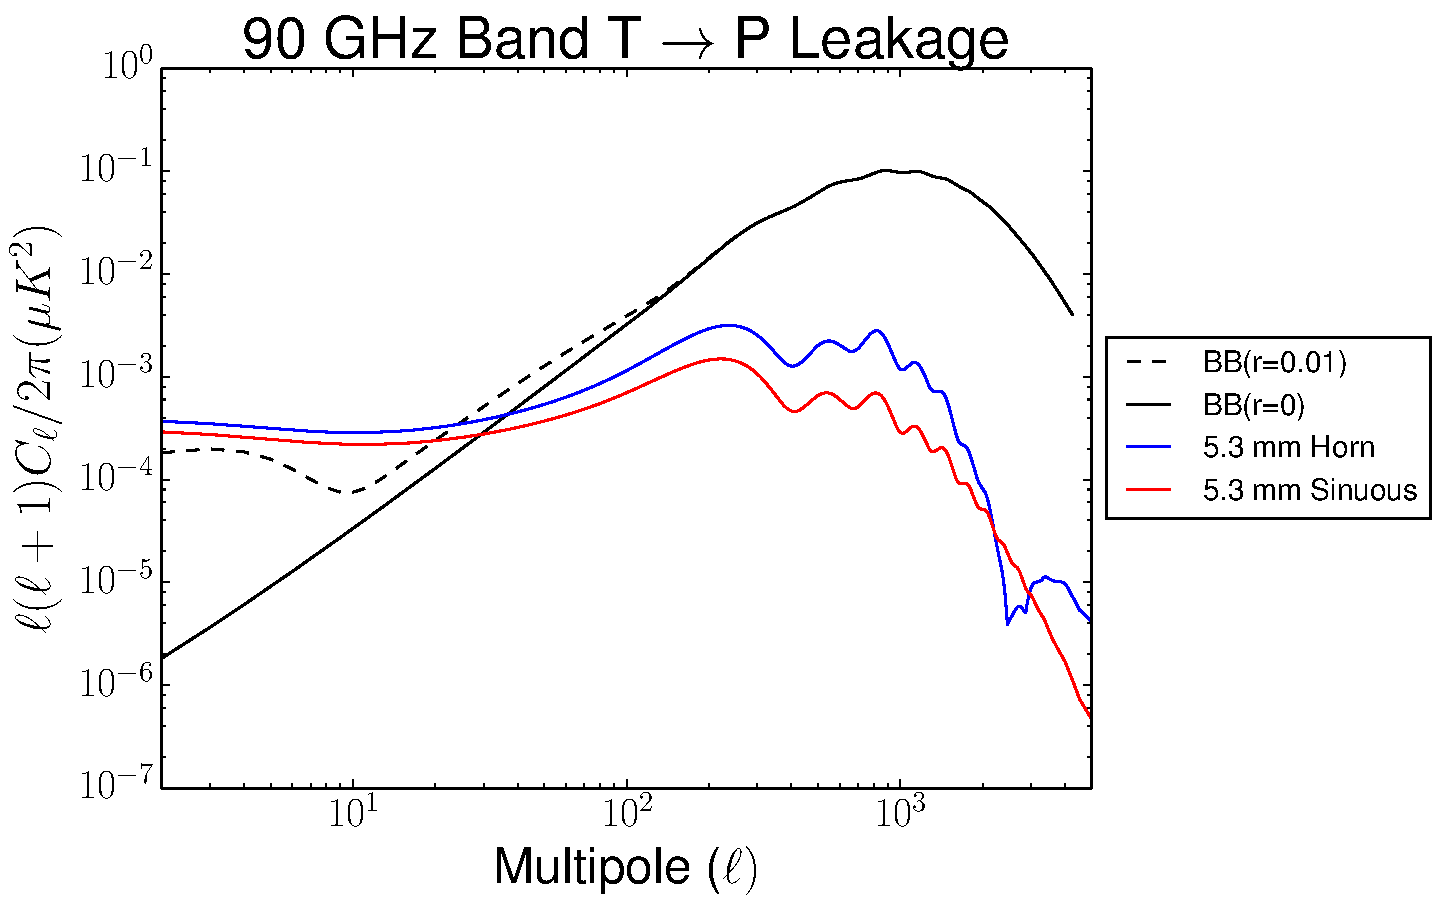
\includegraphics[width=\textwidth]{figures/90GHz_band_ITT_pixel_size_horn_sinuous_5p3mm.pdf}
\caption{The temperature to polarization leakage of the AdvACT spline-profiled feedhorn design (blue) and a lenslet and sinuous design (red) for a 5.3 mm pixel size at 90 GHz. Note that the leakage goes primarily into E-modes for the feedhorn.}
\label{fig:MF_90_TP_leakage}
\end{figure}

\begin{figure}[h!]
\centering
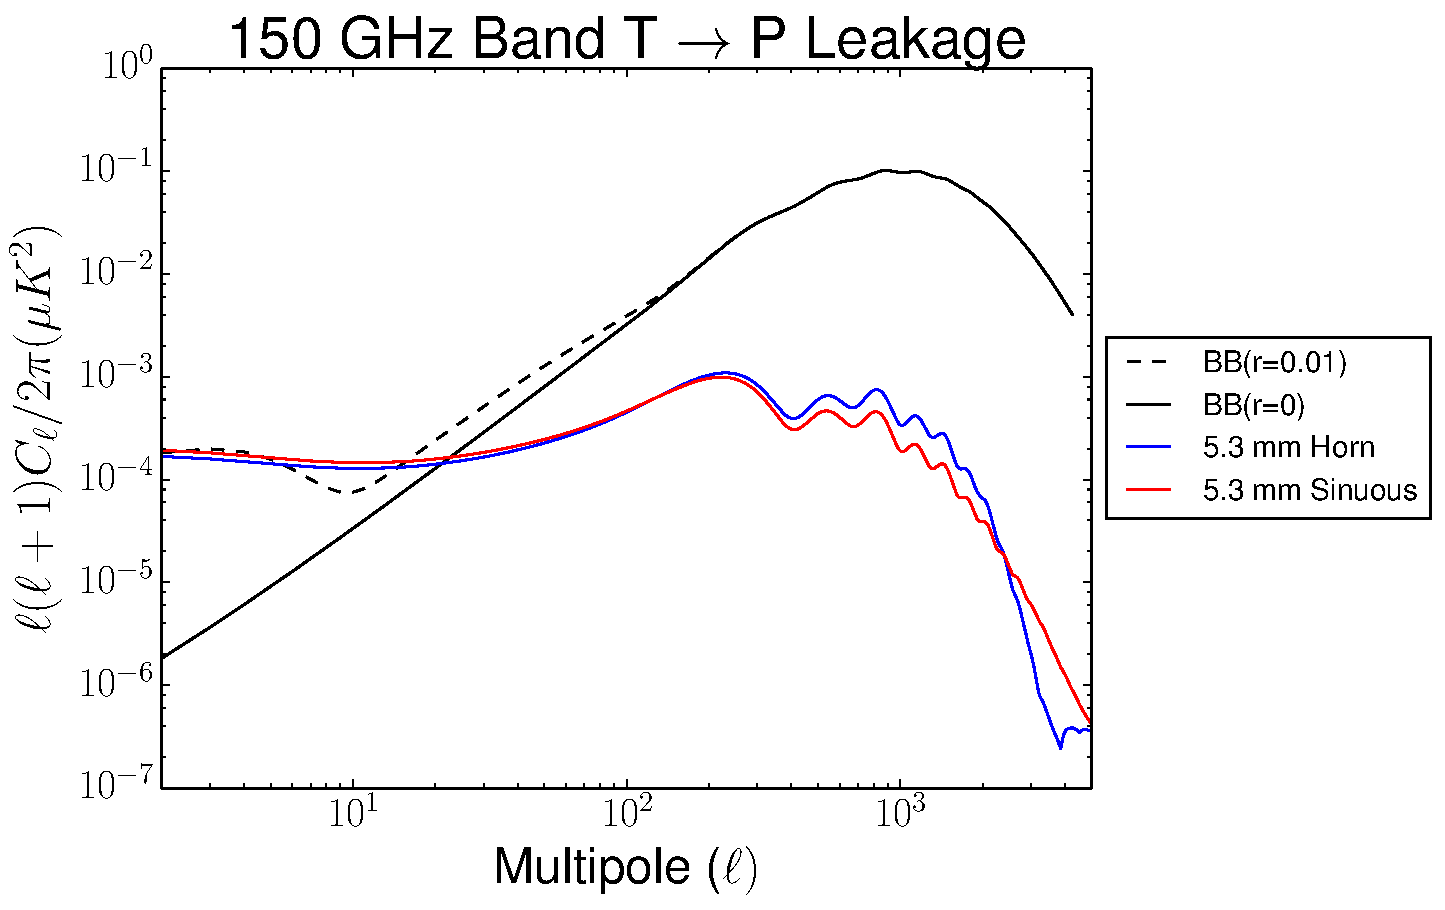
\includegraphics[width=\textwidth]{figures/150GHz_band_ITT_pixel_size_horn_sinuous_5p3mm.pdf}
\caption{The temperature to polarization leakage of the AdvACT spline-profiled feedhorn design (blue) and a lenslet and sinuous design (red) for a 5.3 mm pixel size at 150 GHz. Note that the leakage goes primarily into E-modes for the feedhorn.}
\label{fig:MF_150_TP_leakage}
\end{figure}

\begin{figure}[h!]
\centering
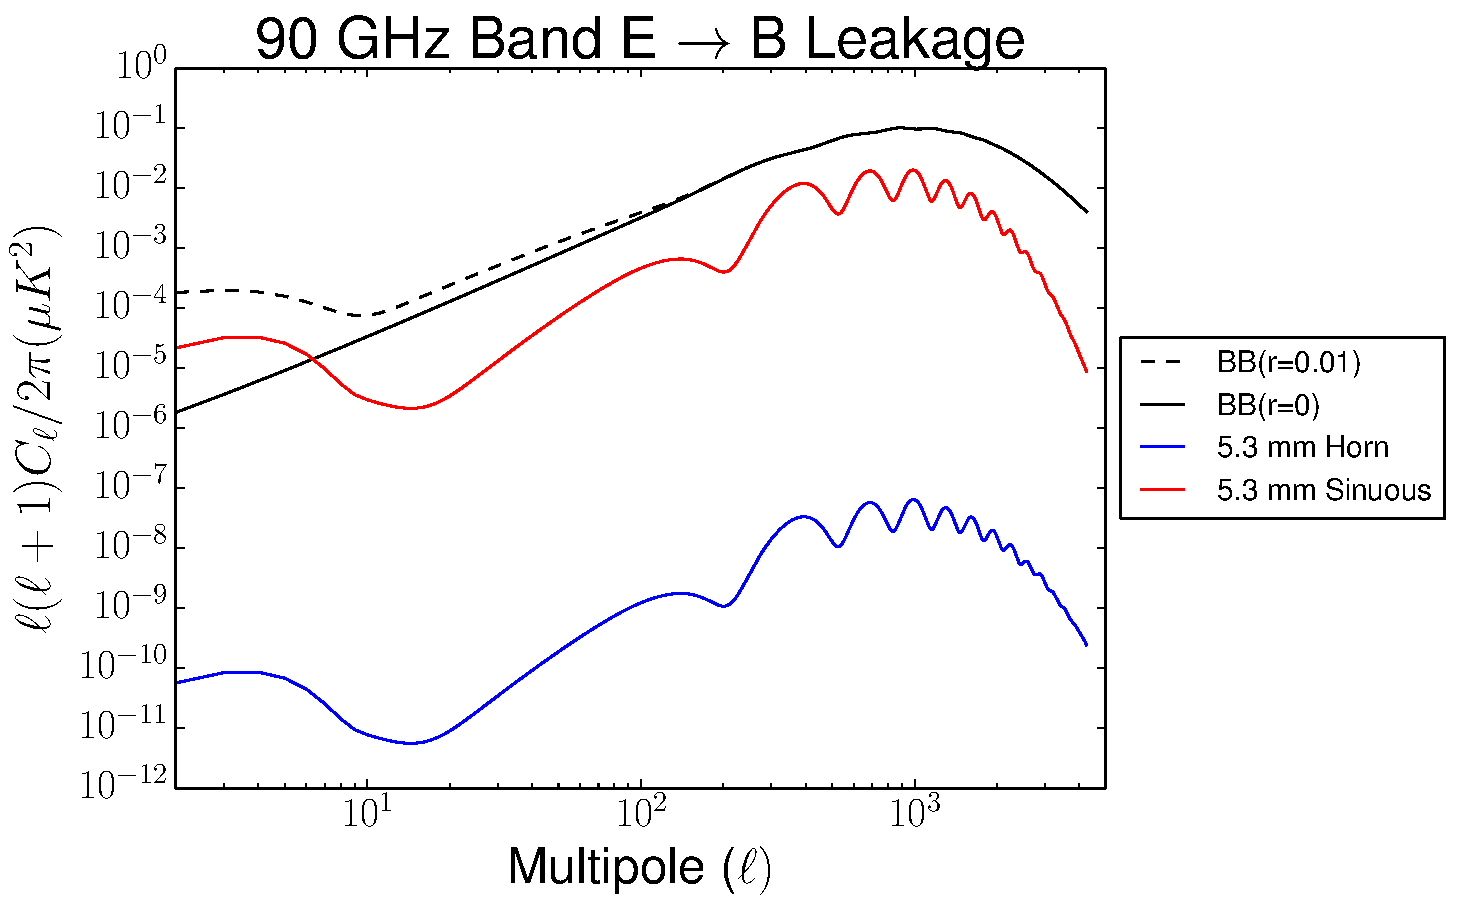
\includegraphics[width=\textwidth]{figures/90GHz_band_UEE_pixel_size_horn_sinuous_5p3mm.pdf}
\caption{The E-mode to B-mode leakage of the AdvACT spline-profiled feedhorn design (blue) and a lenslet and sinuous design (red) for a 5.3 mm pixel size at 90 GHz. Note that the leakage of the feedhorn is negligibly low and that the contribution from the lenslet and sinuous antenna is from the polarization wobble.}
\label{fig:MF_90_EB_leakage}
\end{figure}

\begin{figure}[h!]
\centering
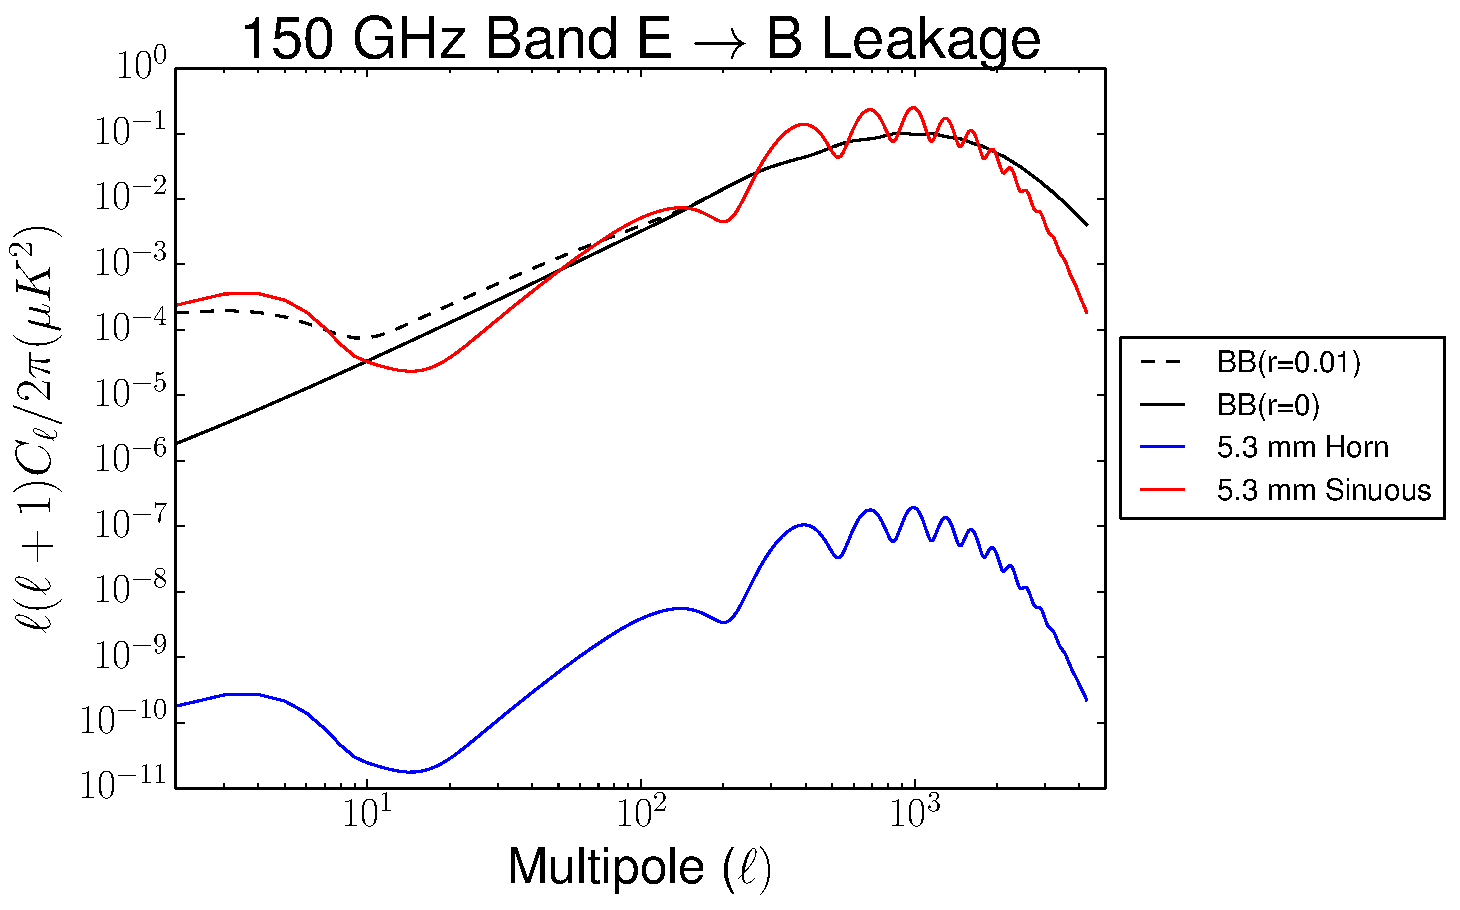
\includegraphics[width=\textwidth]{figures/150GHz_band_UEE_pixel_size_horn_sinuous_5p3mm.pdf}
\caption{The E-mode to B-mode leakage of the AdvACT spline-profiled feedhorn design (blue) and a lenslet and sinuous design (red) for a 5.3 mm pixel size at 150 GHz. Note that the leakage of the feedhorn is negligibly low and that the contribution from the lenslet and sinuous antenna is from the polarization wobble.}
\label{fig:MF_150_EB_leakage}
\end{figure}

\paragraph{Parameterization:}
This can be parameterized with the estimated leakage spectra from the pair-differenced model.


\subsection{Polarization Wobble : Sinuous Antenna}

A sinuous antenna is part of a class of planar antenna geometries called log-periodic antennas due to a log-periodic winding of the antenna arms. The benefit of log periodic antennas is the fact that their properties such as impedance, and beam properties stay consistent over a wide bandwidth and repeat every $ln(\tau)$ where $\tau$ is the characteristic length scale over which the antenna arm pattern repeats. The maximum and minimum bandwidth of these antennas are in theory just set by their inner and outer radii. One characteristic of log periodic antennas that is problematic for polarization measurements of the CMB is polarization wobble. This is a rotation of the polarization axis that oscillates between a maximum and minimum value every $\ln(\tau)$. Within the class of log-periodic antennas the sinuous antenna has the lowest amount of polarization wobble and the amount of antenna wobble is set by $\tau$: lower $\tau$ corresponds to smaller max to min deviation in polarization axis. Detailed studies of the PB2 sinuous antennas can be found in \cite{Obrient2008},\cite{Edwards2012}.


Polarization wobble is primarily a problem because is creates cross polarization or Q to U leakage, which translates into E to B leakage. The wobble can additionally induce temperature to B-mode leakage from the ellipticity angle not alligning with the orthogonal directions of the polarization axis. Systematics from PB2 antennas as well as detectors and lenslets can be found in some details in \cite{TokiThesis}.

\paragraph{Plan to model and/or measure:}
Minimizing $\tau$ minimizes cross polarization but smaller $\tau$ also sets the required linewidths of your traces. For POLARBEAR a $\tau$ of 1.3 was chosen to minimize $\tau$ but still allow for fabrication constraints on trace widths. To further null the effect of cross polarization from polarization wobble a 4 pixel differencing scheme has been proposed \cite{TokiThesis},\cite{TokiMemo1},\cite{TokiMemo2}, which will return Q and U values independent of the polarization wobble angle. This procedure requires two sets of two pixels each (A and B as shown in Fig.~1) with each set having one antenna with one linear polarization oriented at 0 degrees and the second pixel rotated by 45 degrees. The polarization wobble angle is denoted as $\phi(\nu)$, the angle of incident light is $\theta(\nu)$, the detectors efficiency is $\eta(\nu)$, and the electric field amplitude is $E(\nu)$. This setup is depicted in Figure~1. The steps to extract Q and U values for the 4 pixels with the dependence on $\phi(\nu)$ removed is described below. The relative power on the the 90 and 45 pixels of the A and B sets is given by
\begin{figure}
\centering
\includegraphics[width=2.5in]{figures/4pixelremovewobble.png}
\caption{Illustration of 4 pixels with polarization wobble. Each set A and B have both a 0 \& 90 degree orientation antenna and a 45 \& -45 degree orientation pixel. $\theta$ is the polarization angle of incoming light, and $\phi$ is the polarization wobble angle.}
\label{4pixelwobbleremoval}
\end{figure}
\begin{equation}
\begin{split}
&P_{A0} = \int \eta(\nu)[E(\nu)cos(\theta(\nu)-\phi(\nu))]^2 d\nu \\
&P_{A90} = \int \eta(\nu)[E(\nu)sin(\theta(\nu)-\phi(\nu))]^2 d\nu \\
&P_{A45} = \int \eta(\nu)[E(\nu)cos(\frac{\pi}{4}-\theta(\nu)+\phi(\nu))]^2 d\nu \\
&P_{A-45} = \int \eta(\nu)[E(\nu)sin(\frac{\pi}{4}-\theta(\nu)+\phi(\nu))]^2 d\nu \\
&P_{B0} = \int \eta(\nu)[E(\nu)cos(\theta(\nu)+\phi(\nu))]^2 d\nu \\
&P_{B90} = \int \eta(\nu)[E(\nu)sin(\theta(\nu)+\phi(\nu))]^2 d\nu \\
&P_{B45} = \int \eta(\nu)[E(\nu)cos(\frac{\pi}{4}-\theta(\nu)-\phi(\nu))]^2 d\nu \\
&P_{B-45} = \int \eta(\nu)[E(\nu)sin(\frac{\pi}{4}-\theta(\nu)-\phi(\nu))]^2 d\nu .
\end{split}
\end{equation}
We then assume that $\theta$ is constant across our spectral band and difference opposite orientation detectors to extract Q and U:
\begin{equation}
\begin{split}
&Q_A= P_{A0}-P_{A90}=\int \eta(\nu)E^2(\nu)cos[2(\theta-\phi(\nu))]d\nu \\
&Q_B = P_{B0}-P_{B90}=\int \eta(\nu)E^2(\nu)cos[2(\theta+\phi(\nu))] d\nu \\
&U_A = P_{A45}-P_{A-45}\int \eta(\nu)E^2(\nu)sin[2(\theta-\phi(\nu))] d\nu \\
&U_B =  P_{B45}-P_{B-45}\int \eta(\nu)E^2(\nu)sin[2(\theta+\phi(\nu))] d\nu \\
\end{split}
\end{equation}
Using the trig angle sum formula, we can expand this to
\begin{equation}
\begin{split}
&Q_A= \int \eta(\nu)E^2(\nu)[cos(2(\theta)cos(2\phi(\nu))+sin(2(\theta)sin(2\phi(\nu))]d\nu \\
&Q_B = \int \eta(\nu)E^2(\nu)[cos(2(\theta)cos(2\phi(\nu))-sin(2(\theta)sin(2\phi(\nu))]d\nu \\
&U_A = \int \eta(\nu)E^2(\nu)[sin(2(\theta)cos(2\phi(\nu))-cos(2(\theta)sin(2\phi(\nu))]d\nu \\
&U_B =  \int \eta(\nu)E^2(\nu)[sin(2(\theta)cos(2\phi(\nu))+cos(2(\theta)sin(2\phi(\nu))]d\nu . \\
\end{split}
\end{equation}
Taking linear combinations of the above Q's and U's we can define new Q's and U's as
\begin{equation}
\begin{split}
&Q_1=\frac{Q_A+Q_B}{2}= cos(2\theta)\int \eta(\nu)E^2(\nu)cos(2\phi(\nu))d\nu \\
&Q_2 = \frac{U_B-Q_A}{2}= cos(2\theta)\int \eta(\nu)E^2(\nu)sin(2\phi(\nu))d\nu \\
&U_1 = \frac{Q_A-Q_B}{2}= sin(2\theta)\int \eta(\nu)E^2(\nu)sin(2\phi(\nu))d\nu \\
&U_2 =  frac{U_A+U_B}{2}= sin(2\theta)\int \eta(\nu)E^2(\nu)cos(2\phi(\nu))d\nu. \\
\end{split}
\end{equation}
You can then extract $\theta$ as
\begin{equation}
\theta=\frac{1}{2}tan^{-1}\frac{U_{1,2}}{Q_{2,1}}.
\end{equation}
The E-field amplitude can also be determined form this scheme as:
\begin{equation}
E^2=\frac{P_{A0}+P_{A90}}{\int\eta(\nu)d\nu}=\frac{P_{A45}+P_{A-45}}{\int\eta(\nu)d\nu}=\frac{P_{B0}+P_{B90}}{\int\eta(\nu)d\nu}=\frac{P_{B45}+P_{B-45}}{\int\eta(\nu)d\nu}
\end{equation}
Where $\eta(\nu)$ is measured using an FTS. 

The polarization wobble is a large effect that causes significant leakage into the B-mode spectrum, but it is well-understood. It thus needs to be modeled and mitigated, making its SRF a 4.

\paragraph{Uncertainty/Range:}
This analysis assumes that all channels have the same response $\eta(\nu)$, but there is some variation across detectors, so uniformity across the array can limit the effectiveness of this method. This method also requires accurate FTS measurements of the spectral response. It also assumes that the beams are perfectly symmetric, so further uncertainty can be introduced from ellipitical beams. For a trypical sinuous detector, the ellipticity is small with a level of $<2$\% and varies with frequency. \textbf{What are additional sources of uncertainty?}

\textbf{How much suppression of the E to B leakage does this method provide? How much suppression of the T to B leakage does it provide?}

\paragraph{Parameterization:}
The leakage from the polarization wobble can be parameterized as the contaminated Q and U maps to estimate the power spectra leakages. Using the four pixel subtraction method in map space can determine how well these leakages can be mitigated.

\textbf{Make sure these commented out references are in the systematics dictionary references}
%\subsubsection{References}
%\begin{itemize}
%\item O'Brient, B. \textit{et.al.}, "Sinuous-Antenna coupled TES bolometers for Cosmic Microwave Background
%Polarimetry," LTD13 Proceedings (2009).
%\item Edwards, J.M. \textit{et.al.}, "Dual-Polarized Sinuous Antennas on Extended
%Hemispherical Silicon Lenses," IEEE Trans Antennas and Propagation, Vol 60, No 9 (2012).
%\item Suzuki, A. "Lenslet Coupled Sinuous Antenna Systematic Study", Berkeley Memo (2015). - Ask for this, its not published.
%\item Suzuki, A. "Sinuous Antenna Wobble Cancellation", Berkeley Memo (2012). - Ask for this, its not published.
%\item O'Brient, B. \textit{et.al.}, "Sinuous Antennas for Cosmic Microwave Background
%Polarimetry," SPIE, Vol 7020 70201H-1 (2008).
%\item Suzuki, A. "Multichroic Bolometric Detector Architecture for Cosmic Microwave Background Polarimetry Experiments," Berkeley Dissertation (2013).
%\end{itemize} 

\subsection{Absolute Polarization Angle}

\paragraph{Description:}
Absolute Polarization Orientation refers to the polarimeter detectors'
direction measured in celestial coordinates. A miscalibration (i.e. a rotation
bias for the detector orientation) mixes E-modes and B-modes. In addition to
contaminating the CMB polarization power spectra, such a systematic rotation is
degenerate with Cosmic Birefringence (CB) and Cosmic Polarization Rotation
(CPR).

\begin{figure}
\centering
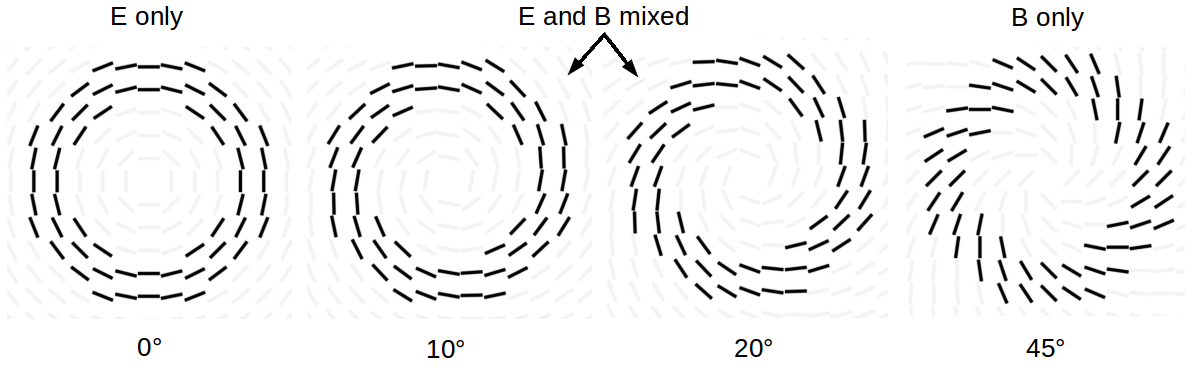
\includegraphics[width=\textwidth]{figures/ebmixing.png}
\caption{Visualization of a coherent polarization angle rotation and its effect on the E and B mode mixing.
}\label{fig:ebmixing}
\end{figure}

Sources of polarization angle systematics are varied and can be introduced
several places in the instrument. A few examples include 1) a rotating
elliptical beam, say in the case of a design incorporating bore-sight
rotations, causing T to P leakage (see ellipticity section); 2) off-axis
refractive optics influencing the propagation of the polarization vectors
according to their Fresnel coefficients, leading to an instrumental
polarization angle rotation; and 3) an apparent polarization angle rotation
from the detector time constants in the presence of a HWP (see time constant
section). Here we focus on 2), namely instrumental polarization errors and
detector polarization angle rotations.


A global polarization rotation is degenerate with a CPR angle and affects the
power spectra as described in \cite{Pagano2009, Keating2013}. 
The effect of a coherent polarization angle roation is to correlate the spectra by an angle $\theta$ such that the new $C'_{\ell}$ coefficients result in

\begin{equation}
\begin{split}
C_{\ell}^{\prime TE} &= C_{\ell}^{TE} cos(2\theta) - C_{\ell}^{TB} sin(2\theta)\\
C_{\ell}^{\prime TB} &= C_{\ell}^{TE} sin(2\theta) + C_{\ell}^{TB} cos(2\theta)\\
C_{\ell}^{\prime EE} &= C_{\ell}^{EE} cos^{2}(2\theta) + C_{\ell}^{BB} sin^{2}(2\theta) - C_{\ell}^{EB}sin(4\theta)\\
C_{\ell}^{\prime BB} &= C_{\ell}^{BB} cos^{2}(2\theta) + C_{\ell}^{EE} sin^{2}(2\theta) + C_{\ell}^{EB}sin(4\theta)\\
C_{\ell}^{\prime EB} &= \frac{1}{2} (C_{\ell}^{EE} - C_{\ell}^{BB}) sin(4\theta) + C_{\ell}^{EB}(cos^{2}(2\theta) - sin^{2}(2\theta))\\
\end{split}
\end{equation}

The standard cosmological model predicts that TB and EB identically vanish.
This prediction can be used to calibrate CMB polarimeters through a
self-calibration method \cite{keating13,kaufman14a}, at the expense of losing
detection capability on genuine physical quantities. This method is
particularly effective for high resolution and/or high sky coverage
experiments. However, the initial assumption is not true in the presence of
phenomena that produce non-vanishing TB and EB. In these cases self-calibration
loses accuracy and introduces biases on cosmological parameters
\cite{abitbol16}. 
Besides, this method destroys the possibility to measure or to place limits on
phenomena that generate TB and EB spectra, like Cosmic Birefringence, Faraday
Rotation and chiral gravity models \cite{kaufman14b,gerbino16}.


\paragraph{Plan to model and/or measure:}

Analytic description of instrumental rotation is challenging, necessitating the
use of optical modeling and experimental techniques for calibration of final
detector angles (absolute and relative) and systematic rotations from the
optics. It is critical to both model and measure the detector polarization angles.
Calibration should be performed before deployment and during observations. 

Modeling of the polarization rotation angle appears feasible and has been used
on ACTPol using Code V \cite{2016arXiv160701825K}. Polarization rotation can be
modeled in CODE V using a polarization sensitive ray trace. An input
polarization is defined and propagated through the optical chain to the
detector focal plane. The pupil averaged Stokes vector is then used to
calculate the polarization angle at the focal plane. This process is repeated
for 25 different fields on the sky and the results are fit to a 2D quadratic.
This fit is then used to estimate the rotation for each detector on the focal
plane. An example of the modeled rotation for the first Advanced ACT array is
shown in Figure \ref{fig:advact_pa4_pol_rotation}. A similar analysis can be
done in Zemax, though is known to not be accurate for fast optical systems.

\begin{figure}[h!]
\begin{center}
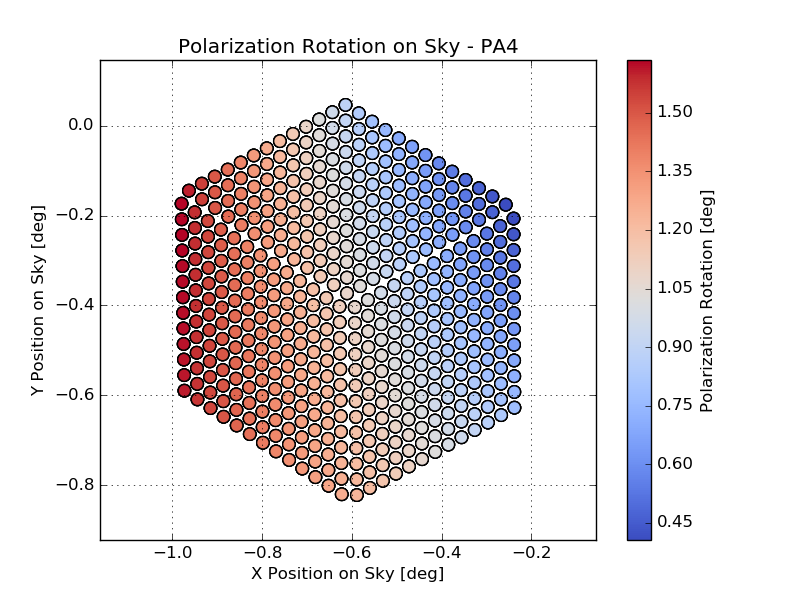
\includegraphics[width=0.60\linewidth]{advact_pa4_polarization_rotation_150ghz_2017.png}
\caption{Modeled instrumental polarization rotation for the high frequency (HF)
Advanced ACT array. Each circle represents a single feedhorn at the focal
plane. The color represents the amount of rotation as modeled by CODE V.}
\label{fig:advact_pa4_pol_rotation}
\end{center}
\end{figure}

This should be checked with physical optics calculations and measurements, but
can be performed on a proposed telescope design which includes both reflectors
and lenses.

Microwave detectors must be cooled down from 300 K to 100 mK, so differential
contractions of the materials in the cryostat limit the accuracy of their
aligment. It is also critical to refer the detector orientation with respect
to the telescope and the receiver mount once the cryostat is closed. As a
result, direct polarization angle calibration is not possible with an accuracy
better than 1$^{\circ}$.

We plan to use polarization calibrators in-lab while testing full optics tubes
before deployment, in situ in the field with polarization calibrators, either
through a ground-based calibrator, or utilizing a flying artificial source, and
observations polarized astrophysical sources. However, natural sky sources
traditionlly used to calibrate the absolute polarization angle suffer from
frequency dependence and time variability. The best option are Tau-A and Cen-A,
but they allow an accuracy for the polarization orientation between 1$^{\circ}$
and 0.5$^{\circ}$ \cite{planck16i,polarbear14,weiland11}. 

Placing a well known polarization calibrator in the far field of the telescopes
is the optimal approach, though quite challenging. Proposed ideas include
operating precisely characterized, linearly polarized microwave sources using a
drone, a balloon, or a CubeSat \cite{nati2017, Johnson2015}. These artificial
calibrators will match the sensitive frequency bands of the polarimeters and
will be observed at high elevation angles, far from Earth signal contamination.

The source is coupled to an attitute control system making use of star cameras
and other attitude sensors. The caibrator will utilize two celestial
coordinates (from the accurate star camera pointing direction) to determine the
third angle defining the rotation of the polarization plane along the
detectors' line of sight. The telescopes' detector orientation is then measured
by observing the calibration source signal. 

\textbf{Say something about the PB calibrator that Grant has been working on}.


Alternative calibrators require placement in the near field and include
sparse/dense wire grid polarizers or dielectric sheets \cite{Takahashi2010,
2016arXiv160701825K}.  However, any strategy based on optical elements placed
between the mirrors and the polarimeter does not allow to measure the polarized
beam systematics induced by the warm optics. 

\textbf{Note that it would be easier to measure in-lab if we only have the
optics tubes and what options we have for that. See the calibration hardware
spreadsheet linked on the CSS telecon page.}

The absolute calibration of the polarization angle is critical for the
detection of inflationary gravitational waves, the constraining power on the
neutrino sector through measurements of gravitational lensing of the CMB, the
possibility of detecting Cosmic Birefringence (CB), and the ability to measure
primordial magnetic fields, and thus has an SRF of 5.

\paragraph{Uncertainty/Range:}
%This section should include the uncertainty of
%known parameters and/or the expected range of parameters for consideration

Angle offsets $\sim 1^{\circ}$ produce spurious B-mode signal at the same level
as primodial B-modes for a tensor to scalar ratio of $r \sim 0.005$ as well as
nonzero $EB$ and $TB$ cross-correlations \cite{doi:10.1142/S0218271816400125}.
Currently employed calibration methods provide calibration to at
best $0.5^{\circ}$ \cite{2016MNRAS.455.1981K}.
Calibration to better than $0.05^{\circ}$ would allow for constraints on CB of
order one degree to greater than $15\sigma$ \cite{2016MNRAS.455.1981K}.

A miscalibration of 0.5$^{\circ}$ in the polarization orientation translates
into a spurious B-mode signal corresponding to a tensor-to-scalar ratio of $r
\simeq 0.01$ \cite{abitbol16}, affecting the SO sensitivity range.  Depending
on the targeted value for r, we need to calibrate the polarization angle with
arcmin or even sub-arcmin accuracy. 
A simulated result is shown in Fig. \ref{plot_r:fig} \cite{nati2017}, for an
ACT-like and a CMB-S3 experiment. Assuming  the red curve represents a false
bias signal introduced by a miscalibration of 1$^{\circ}$ (i.e., the current
accuracy) in the orientation of the detectors.  The bias starts to emerge above
the statistical uncertainty for ACTPol sensitivity (the image on the left). For
CMB-S3 (the image on the right), the new generation of ground experiments, the
bias is well above the sensitivity and it dramatically affects the measurement
of r. If the same experiment benefits from a calibration with accuracy between
0.01$^{\circ}$ and 0.001$^{\circ}$, the bias can be recovered as represented by
the blue region.
 
\begin{figure}[ht]
\begin{center}
\includegraphics[width=\textwidth]{figures/act_s3_r} 
\end{center}
\caption{Assuming no gravitational waves, the red curve in these simulations
represents a false detection of $r$ caused by the polarization angle
miscalibration of 1$^{\circ}$. With a calibration accuracy between
0.01$^{\circ}$ and 0.001$^{\circ}$ represented by the blue region, POLOCALC
\cite{nati2017} recovers the fiducial value of r=0 (the black dashed curve).
The uncertainty on the value of $r$ will be then limited by the sensitivity of
the experiment. The false bias already starts to emerge above the statistical
uncertainty for the ACTPol sensitivity, while for CMB-S3 it dramatically
affects the measurement of the tensor-to- scalar ratio. For CMB-4 the gap is
going to increment.}
\label{plot_r:fig}
\end{figure}

\paragraph{Parameterization:}
This effect can be parameterized by the polarization angle uncertainty, which
can be used to estimate the polarization power spectra leakages as in
\cite{nati2017}. This can be used to estimate the impact on our
science goals.

cience goals.

\subsection{Inhomogeneous AR Coating}

\paragraph{Description:}
If a telescope has any transmissive opitcal elements, those elements will need to have an effective antireflective (AR) coating.  Some systematics are particular to the AR technology used, but there are some general systematics.  Inhomogeneities can occur with most technologies, such as by a variation in the thickness of a layer across the element.  This will cause a decrease in the AR performance at the location of the inhomogeneity.  If the element is in a position in the beam such that all the detectors effectively see the entire element, this will be averaged over the entire element, and the systematic will be the same across the whole focal plane.  If the element is in a position such that each detector sees only a small part of the element, there will be a focal plane positional dependence on the transmission.  If there are several such elements in the optical path for each detector, the effect will hopefully average out over the focal plane.

\paragraph{Plan to model and/or measure:}
The AR coating performance of each element can be measured with a reflectometer. Measurements of specific technologies can give the tolerances of each technology. Using reflectometery, we can measure reflection vs. frequency data for these designs, understand the thickness and index tolerances of any proposed AR technology, and determine an rms for each layer of AR coating. Using the tolerances, rms values, and a transfer matrix model can give predictions on how much this will affect the overall AR coating performance. Given the reasonably tight tolerances of current technologies, this will not be a major problem and thus has a SRF of 2.

\paragraph{Uncertainty/Range:}
Most technologies can get to a paricular thickness consistency across the surface. This may be from $\pm$ 5 to 25 $\mu$m depending on the technology. Overall, this is a relatively small amount at most frequencies though at the upper end of ground-based range, it may start to present a problem. If the AR performance is tightly tuned across the band (to about 0.5\% or less across the band), then any deviation will cause the the performance to degrade to $\sim 1$\%. If the performance is closer to $\sim 1$\% or the coating has a very broad bandwidth, then this effect will shift the performace bands around by a few percent.  

\paragraph{Parameterization:}
The transfer matrix formalism with the measured tolerances and rms can give the total impact on the AR coating performance.

\subsection{Reflector Spillover}

\paragraph{Description:}
Reflector spillover corresponds to detector illumination by photons that do not propagate through the regular optical chain by hitting the primary, secondary, etc. This type of signal can be reduced through proper optical design procedures, but is challenging to remove entirely in a reflector system.

\paragraph{Plan to model and/or measure:}
Typically, reflector spillover is modeled through ray tracing techniques using an accurate CAD model of the telescope. Unless the spillover amplitude is high, it can be challenging to isolate and map spillover across the spatial response of the telescope. Depending on the amplitude of the spillover, it could be possible to isolate its value by observing a point source.

This effect is more significant in reflector systems and can be significant, especially in the instrument sensitivity, so it has an SRF of 4.

\paragraph{Uncertainty/Range:}
\textbf{Need some values for the SO LAT and SAC.}
\paragraph{Parameterization:}
Spillover can be quantified by the total amount of beam solid angle contained in spillover regions, $\Omega _\mathrm{spill}$ relative to the total beam solid on the sky $\Omega _\mathrm{total}$. For CMB experiments, a ratio of $\Omega _\mathrm{spill} / \Omega _\mathrm{total} > 0.01$ should be considered quite large.

\subsection{Ruze Scattering} \label{sec:ruze}

\paragraph{Description:}

Gaussian surface errors on reflector elements redistribute power from the main beam to larger angles. Errors with large spatial correlation lengths (large dimples), compared to the wavelength of reflected light, will distribute energy to relatively small angular scales. Conversely, small dimples will distribute energy over large angular scales. The beam shoulder generated this way is often called a Ruze-envelope. Ruze derived an expression for loss in antenna gain due to uncorrelated surface errors with a Gaussian distributions of zero mean deformations spanning a range of physical scales. The expression appropriate for the beam response is \cite{Ruze1966}
\begin{equation} 
\Psi(\theta,\phi) = \Psi_0(\theta,\phi) e^{-\overline{\delta^2}} + \left( \frac{2 \pi l}{\lambda} \right)^2 e^{-\overline{\delta^2}} \sum_{n=1}^{\infty} \frac{\overline{\delta^2}^n}{n \times n!} e^{-\left(\pi l \sin(\theta) / \lambda \right)^2/n},
\label{eq:gr}
\end{equation}
where $l$ is the correlation length of the surface deformation, $\lambda$ is the wavelength, $\Psi_0(\theta,\phi)$ is the ideal beam shape and $\overline{\delta^2}$ represents the variance of the phase errors. The equation is applicable in the limit when $D/(2l) \gg 1$, where $D$ is the diameter of the optical element. According to Equation \ref{eq:gr}, loss in forward gain is mainly determined by the amplitude of the RMS error and not correlation lengths.

Since random surface errors have a tendency to create an azimuthally symmetric sidelobe, Ruze scattering can create a relatively benign systematic. However, large surface errors remove power from the main beam in a way that reduces the forward gain of the telescope and therefore the telescope sensitivity.

\paragraph{Plan to model and/or measure:}
Surface errors on reflectors can be measured through interferometry and photogrammetry techniques \cite{Hincks2008, Tauber2010}.

\paragraph{Uncertainty/Range:}
Since the effect of surface errors depends highly on frequency, acceptable surface error RMS values depend on the operational frequency of the telescope. For the reflectors on the Planck satellite, the RMS error var measured to be smaller than 10 $\mu$m \cite{Tauber2010}. The ACT collaboration has reported surface errors ranging from 10--30 $\mu$m \cite{Hincks2008}. \textbf{What is the spec on the mirror RMS for the SO LAT?}

\paragraph{Parameterization:}
We parametrize this effect using the surface error variance $\overline{\delta^2}$ and associated correlation lengths $l$ (see equation \ref{eq:gr}). 



\section{Spectral Response Function}
\subsection{Bandpass Mismatch}

\paragraph{Description:}
Different detectors can have different bandpasses from effects like fabrication variations. 

%The total power received by a detector is the sum of each source of light coming from the sky integrated over the bandpass of the detector. Given that each component of the signal has a different spectrum, the calibration of the detector is component dependent. For each component $k$ and bolometer $b$, we can define a transmission coefficient
%\begin{equation}
%C_k^b = \frac{\int S_k(\nu) F(\nu)}{\int S_{CMB}(\nu) F(\nu)}.
%\end{equation}
%These correction factors to the gain should be applied whenever the signal has a different frequency dependance than the CMB. If not accounted for, this will result in a mis-calibration like effect for all of the foregrounds, producing temperature-to-polarization and polarization-to-polarization leakage.

Power spectra leakages also manifest when two detectors with non-identical spectra are pair-differenced to get a polarized signal. \textbf{expand on this a bit}

\paragraph{Plan to model and/or measure:}
The only way to mitigate this effect is with spectral measurements of the detector bandpasses using a Fourier Transform Spectrometer (FTS). For these measurements to be effective, we must have wide coverage across each array so that we can characterize any wafer variations and better understand idividual detector bandpasses. FTS measurements for each detector should be performed in the lab prior to deployment and in situ in the field.

\textbf{Discuss how the size of a mismatch can be modeled by changing the dielectric thickness in the filter to model fabrication variance. Describe how with this, we can model the maximal band offset, with that, we can tell how well we need to know the detector bandpasses. Discuss how this can then be used to set FTS calibration requirements and also for requirements on detector fab array uniformity.}
%Using external foregrounds maps as templates, the leakage maps can be computed and subtracted. However, this method is limited by our knowledge of the foregrounds, and the external available data. Simulations to estimate the level of leakage and set a constraint on the differential bandpasses should be performed.

This effect can cause polaization leakage and requires thorough instrumental calibration, making its SRF a 4. This effect is less worrying when pair-differencing is not used, as in the case of a HWP, which brings its SRF down to 3.

\paragraph{Uncertainty/Range:}
\textbf{How well do we need to know each detector bandpass for the spectral effect? for pair differencing? What requirements do these put on FTS calibration? Do we need R and D to reach these levels of calibration or are we already there? How much of an array do we need to understand? Do we need FTS measurements of every array?}

\paragraph{Parameterization:}
This effect can be parameterized as an uncertainty on the center frequency and bandwidth of the detectors, which can be used to estimate the limitations on the proposed science, particularly on how well we can constrain $r$.

\subsection{Bandpass Changes due to Atmosphere}

\paragraph{Description:}
Atmospheric variables including precipitable water vapor (PWV), observing angle, and ground temperature can have significant effects on telescope observing conditions when making measurements of the Cosmic Microwave Background radiation.  More specifically, changes in the opacity of the atmosphere lead to variations in the effective gain of the instrument's bandpass.  Furthermore, these changes in opacity are frequency dependent, which lead to shifts in the central frequency of the instrument's bandpass.  Both band gain and central frequency are important factors in the data-to-map analysis pipeline, and any uncertainties in these values must be well understood.

\paragraph{Plan to model and/or measure:}
In order to model the effect of atmospheric changes on detector bandpasses, we first need to model the transmission of the atmosphere across the frequencies of interest.  This is accomplished by using the am Atmospheric Model code developed by Scott Paine from the Harvard-Smithsonian Center for Astrophysics.  The code comes equipped with various templates, one of which being the Chajnantor Plateau in Chile where the Simons Observatory will be located.  Several environmental parameters can be adjusted such as precipitable water vapor (PWV), zenith angle, and ground temperature.  The output of the code gives the transmission of the atmosphere vs frequency.  Figure \ref{transmissions} shows the plotted output for varying the PWV at a fixed ground temperature and zenith angle.   

Figure \ref{transmissions} also shows the average bandpasses for ACTPol 20, 40, 90, 150, and 220 GHz detectors.  With models of the bandpass, atmosphere transmission, and estimated spectrums of what we plan to observe (CMB, dust, etc.), we can then quantify variations in the band gain and centers caused by changing atmospheric conditions.  Figure \ref{transmissions} also shows the average bandpasses for ACTPol 20, 40, 90, 150, and 220 GHz detectors.  With models of the bandpass, atmosphere transmission, and estimated spectrums of what we plan to observe (CMB, dust, etc.), we can then quantify variations in the band gain and centers caused by changing atmospheric conditions.

\begin{figure}[h] %  figure placement: here, top, bottom, or page
   \centering
   \centerline{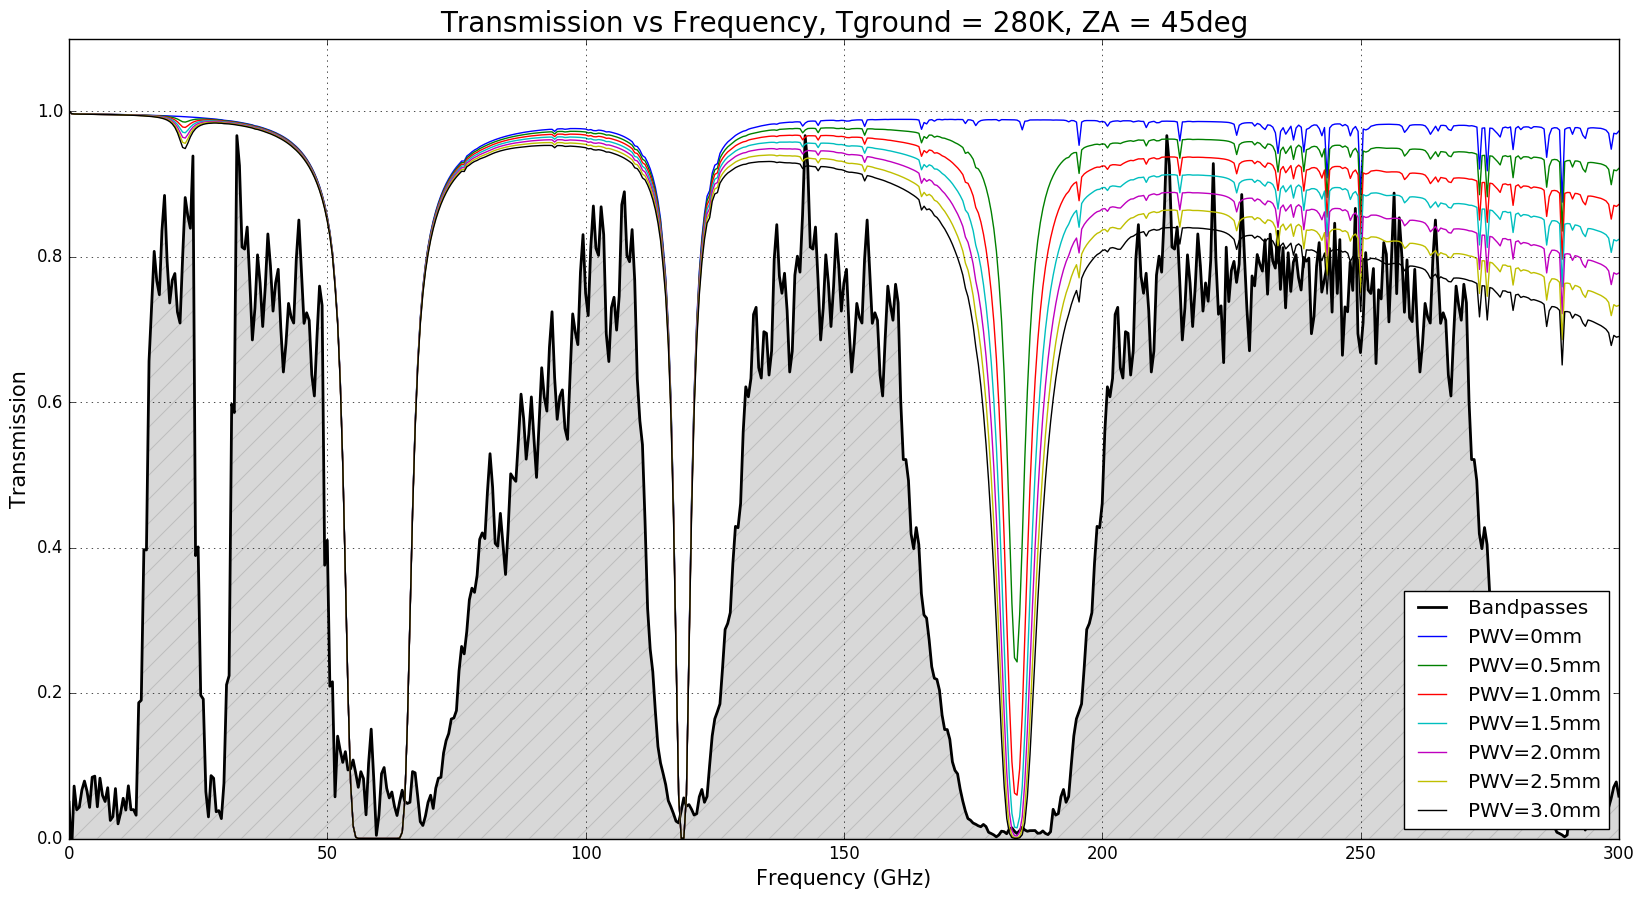
\includegraphics[width=\linewidth]{test.png}} 
   \caption{Atmosphere transmission lines and averaged bandpass for 20, 40, 90, 150, and 220 GHz channels.  A colored transmission line is plotted for each value of PWV while holding the observing angle and ground temperature constant.}
   \label{transmissions}
\end{figure}

\paragraph{Uncertainty/Range:}
To calculate the changes in band due to atmospheric variations, the average bandpasses are multiplied by the atmosphere transmission lines.  We then compute the integrated power and central frequency of each of the five bands for each case.  For total atmosphere effects, the three parameters of PWV, ground temperature, and observing angle are combined together to estimate the minimum (smallest change to FTS measured band) and maximum (largest change to FTS measured band) observing conditions experienced during data collection.  The minimum change parameters are defined to be PWV = $0$mm, Tground = $290$K, and ZA = $30$deg and the maximum change parameters to be PWV = $3$mm,Tground = $250$K, and ZA = $60$deg.  These values correspond to the best and worst possible atmospheric conditions in useable data throughout a full observing season.  For example, data where PWV > 3mm is automatically discarded for ACT science analysis.  Figure \ref{minmax_bands} shows the resulting bands for the minimum and maximum cases described above.  

The bands also change depending on the spectrum of the observed source.  In addition to simulating changes in the measured detector band alone, the band gain and band centers are also calculated for the detector bands multiplied by the CMB spectrum and the detector bands multiplied by an estimated dust spectrum $(\nu^{2.9})$.  It is important to test the changes for each observed source to identify whether or not the same calibrations can be used for all sources.  The top row in Figure \ref{minmax_bands} shows the minimum and maximum band changes for the measured band alone, the middle row shows the changes for an estimated dust spectrum, and the bottom row shows the changes for the CMB spectrum.

\begin{figure}[H]
\centering
 \begin{varwidth}{\linewidth}
 \subfloat{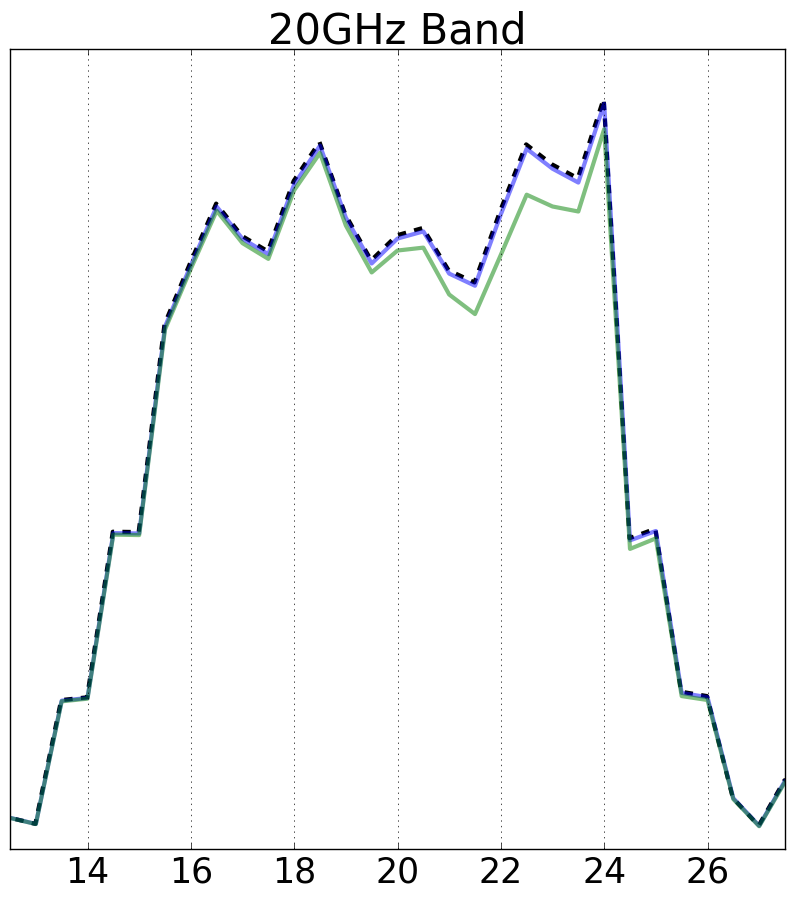
\includegraphics[width=.2\linewidth]{minmax_totals_20GHz.png}}
 \hspace{-2.5mm}
 \subfloat{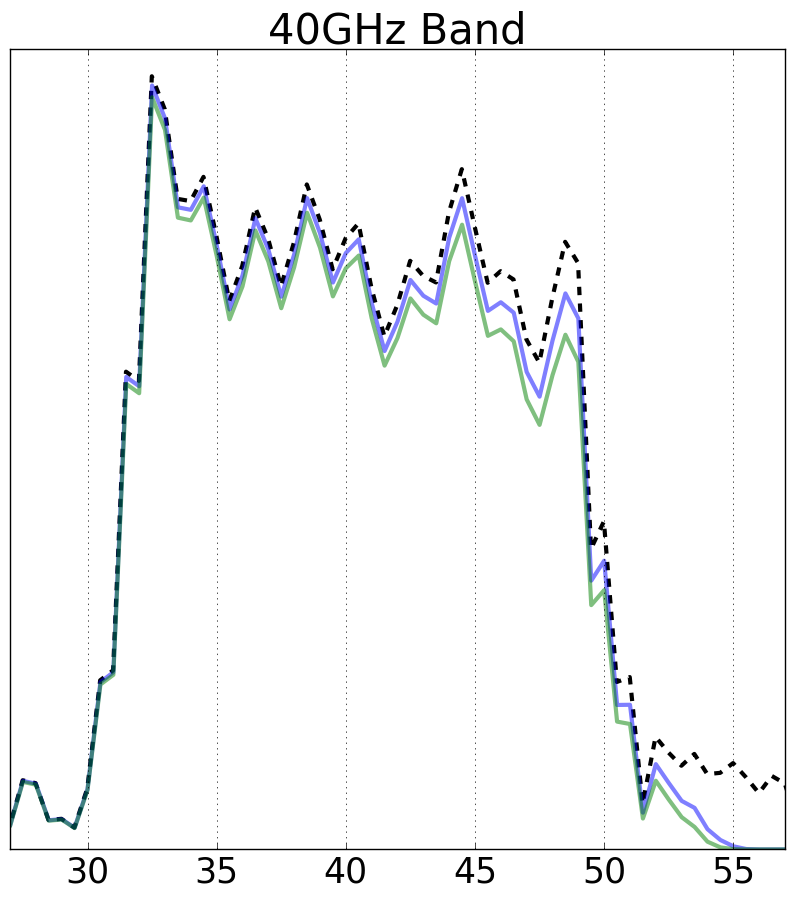
\includegraphics[width=.2\linewidth]{minmax_totals_40GHz.png}}
 \hspace{-2.5mm}
 \subfloat{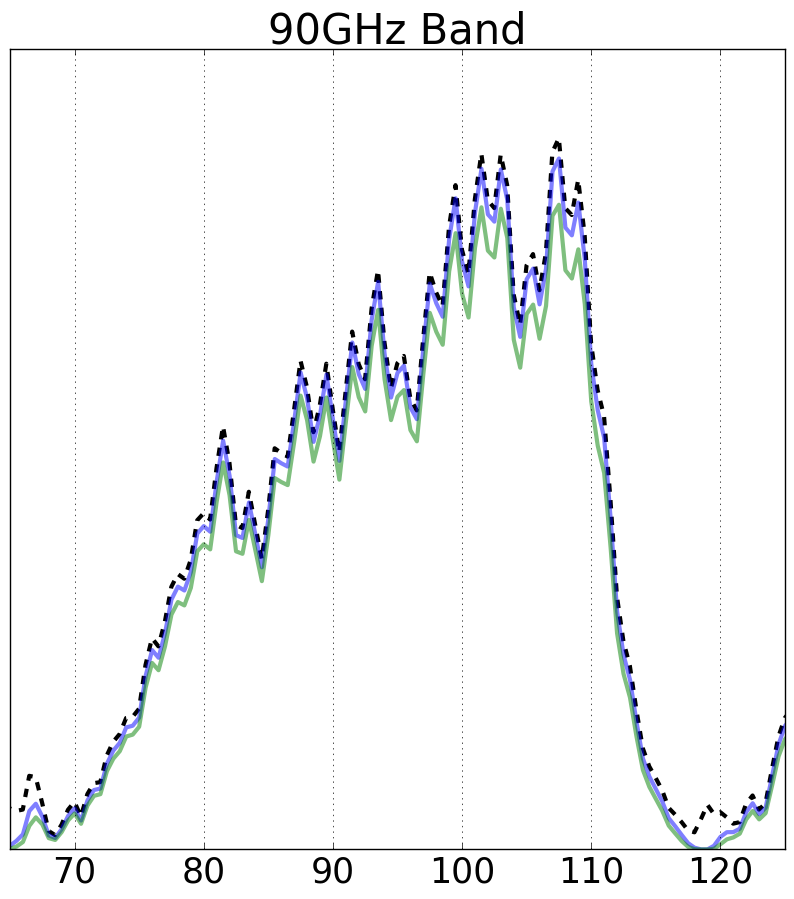
\includegraphics[width=.2\linewidth]{minmax_totals_90GHz.png}}
 \hspace{-2.5mm}
 \subfloat{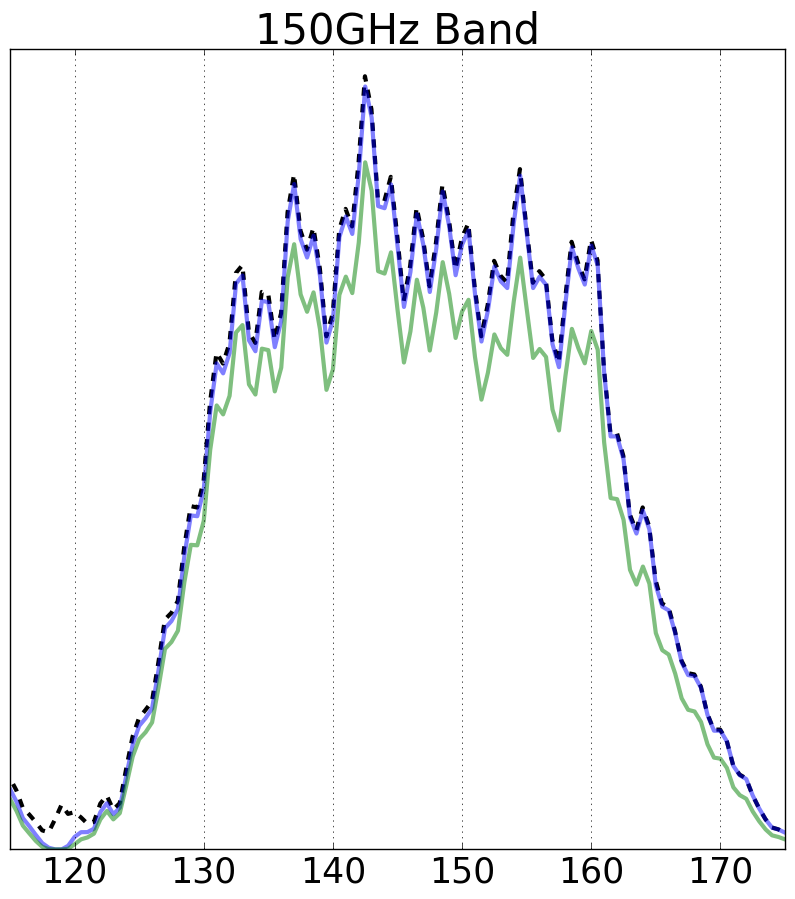
\includegraphics[width=.2\linewidth]{minmax_totals_150GHz.png}}
 \hspace{-2.5mm}
 \subfloat{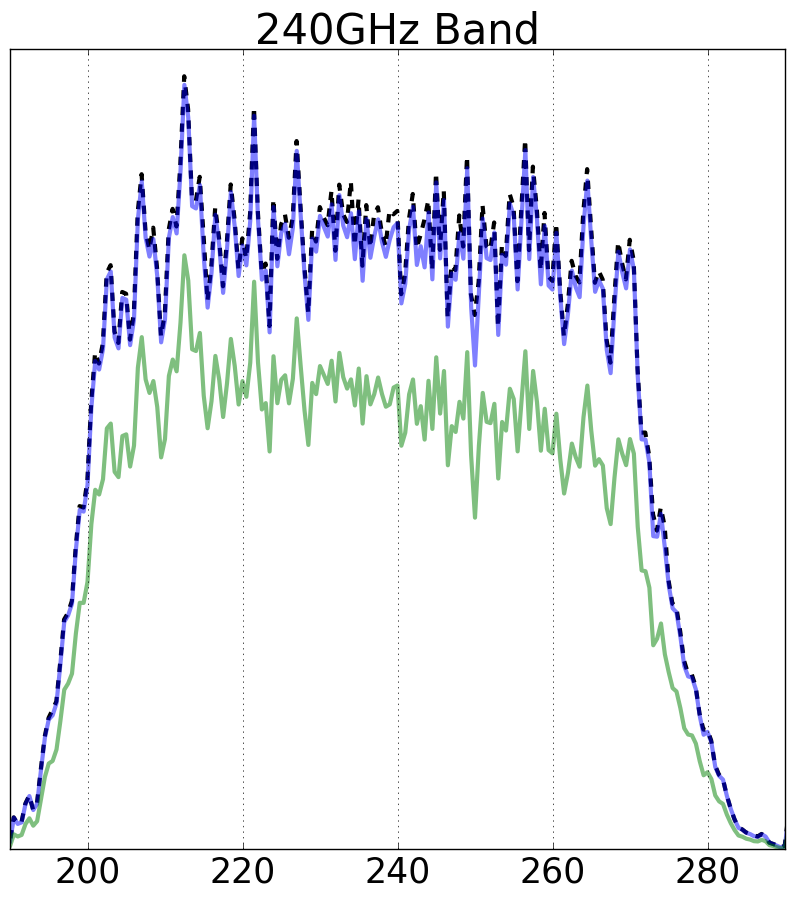
\includegraphics[width=.2\linewidth]{minmax_totals_240GHz.png}}
 \end{varwidth}
 \begin{varwidth}{\linewidth}
 \subfloat{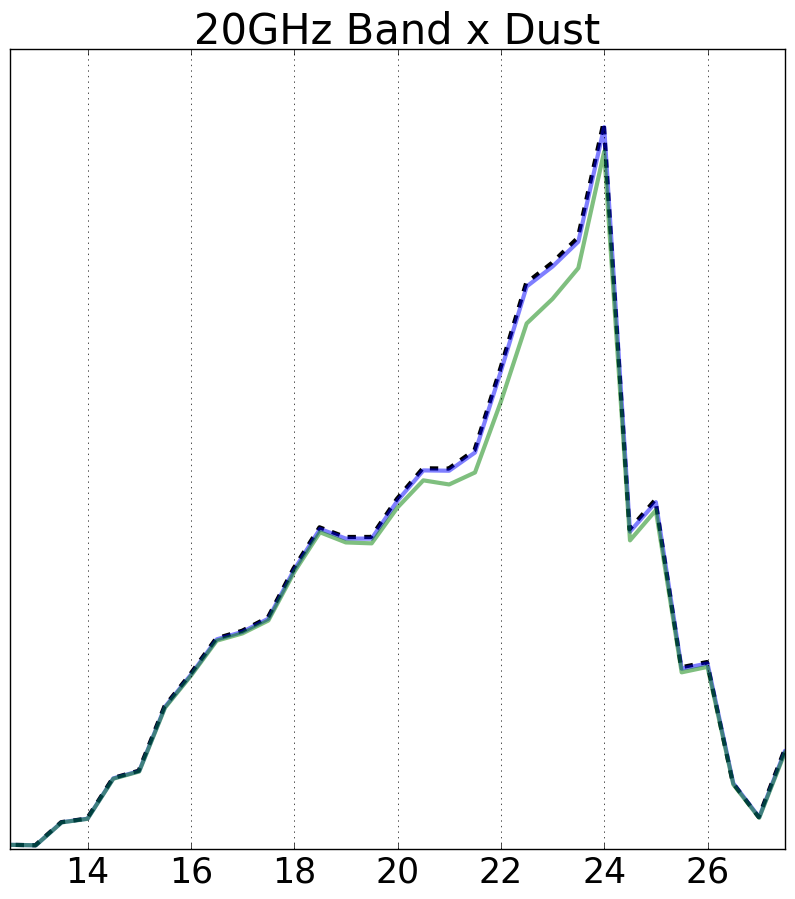
\includegraphics[width=.2\linewidth]{minmax_totals_20GHz_dust.png}}
 \hspace{-2.5mm}
 \subfloat{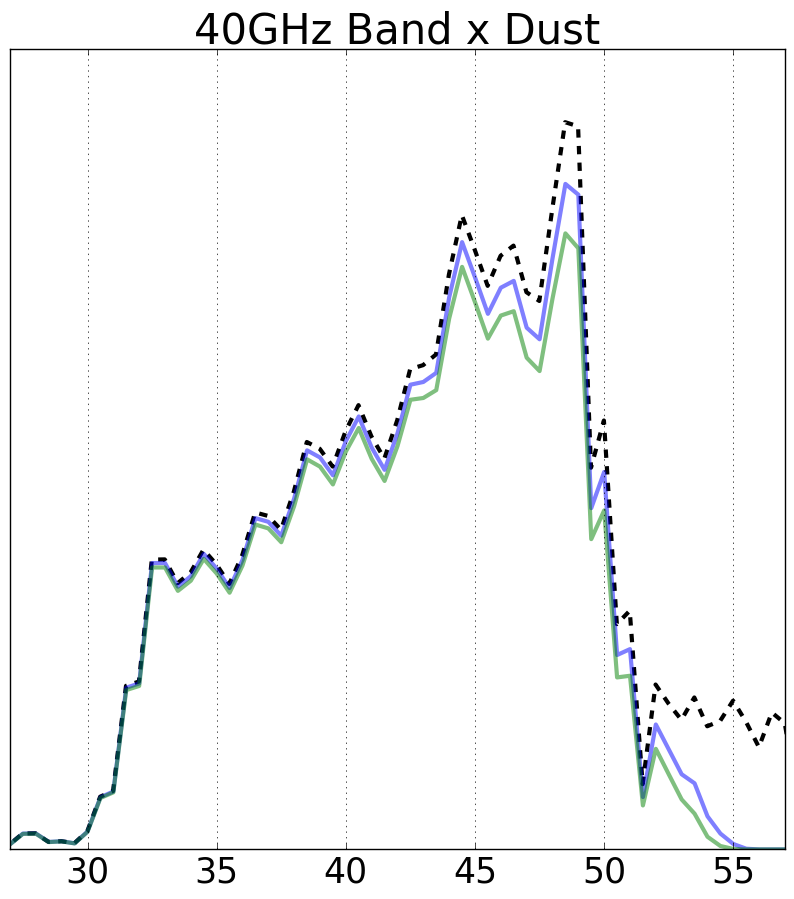
\includegraphics[width=.2\linewidth]{minmax_totals_40GHz_dust.png}}
 \hspace{-2.5mm}
 \subfloat{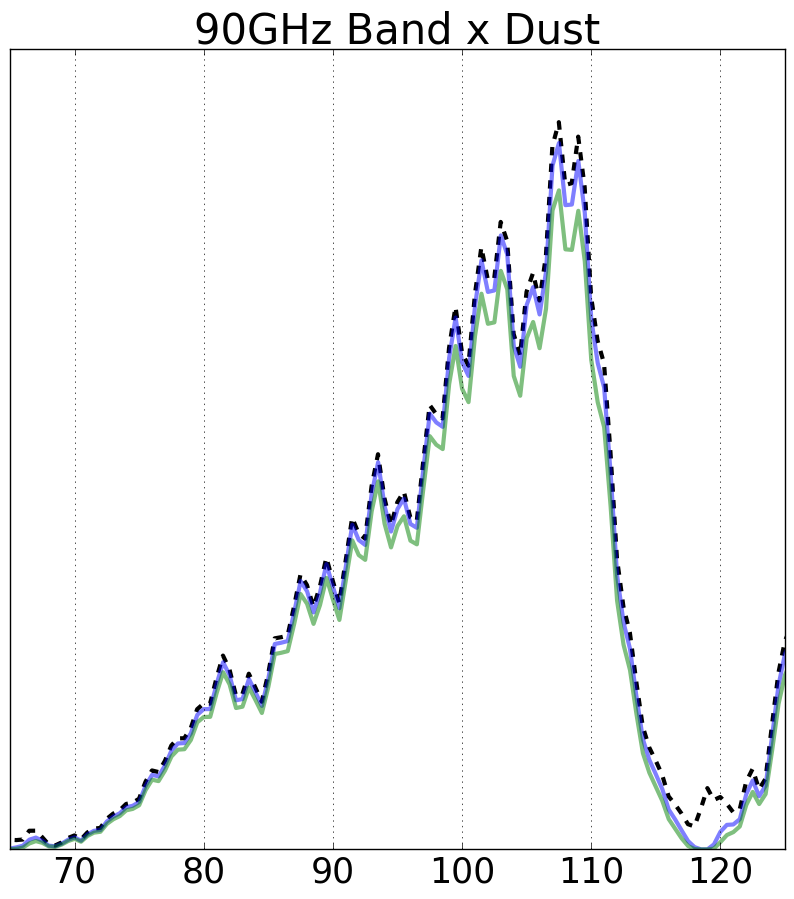
\includegraphics[width=.2\linewidth]{minmax_totals_90GHz_dust.png}}
 \hspace{-2.5mm}
 \subfloat{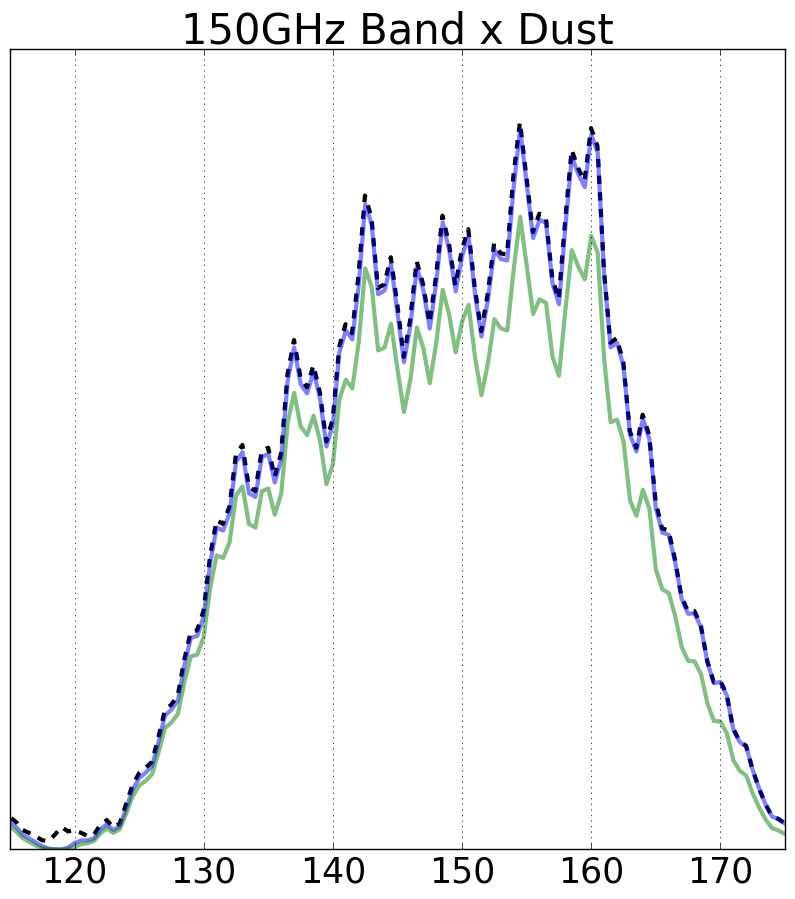
\includegraphics[width=.2\linewidth]{minmax_totals_150GHz_dust.png}}
 \hspace{-2.5mm}
 \subfloat{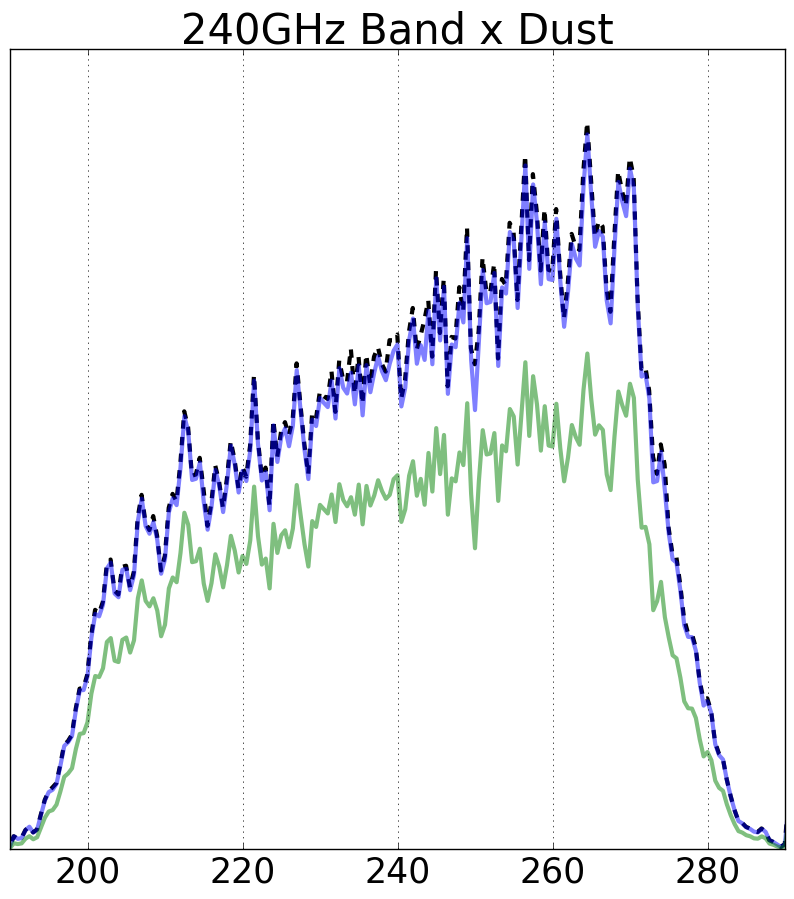
\includegraphics[width=.2\linewidth]{minmax_totals_240GHz_dust.png}}
 \end{varwidth}
 \begin{varwidth}{\linewidth}
 \subfloat{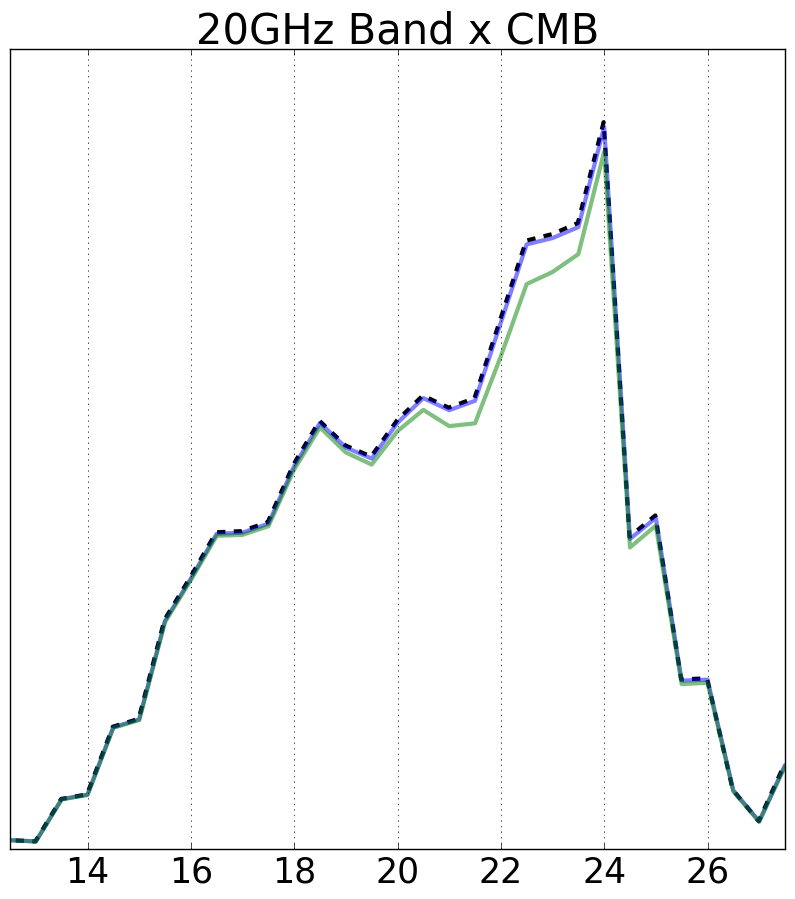
\includegraphics[width=.2\linewidth]{minmax_totals_20GHz_cmb.png}}
 \hspace{-2.5mm}
 \subfloat{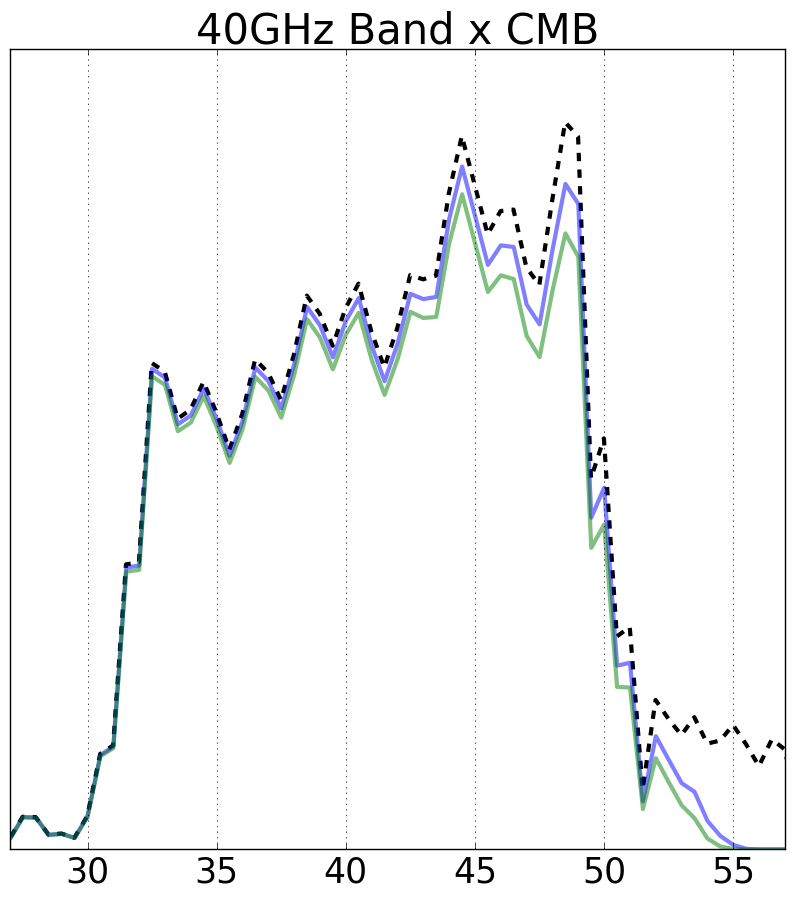
\includegraphics[width=.2\linewidth]{minmax_totals_40GHz_cmb.png}}
 \hspace{-2.5mm}
 \subfloat{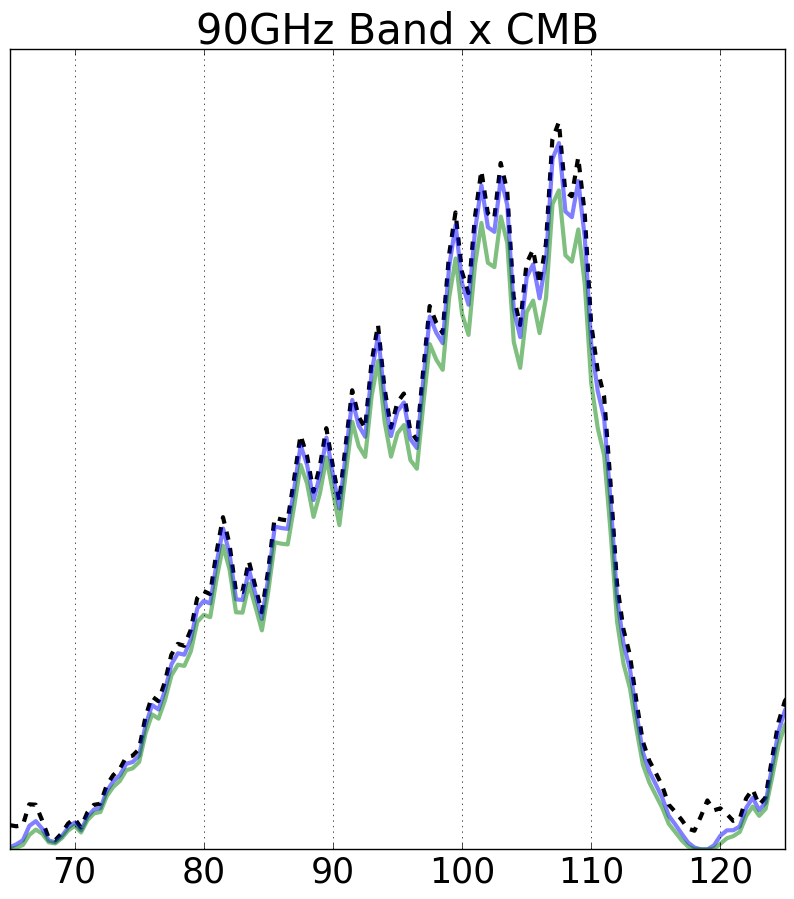
\includegraphics[width=.2\linewidth]{minmax_totals_90GHz_cmb.png}}
 \hspace{-2.5mm}
 \subfloat{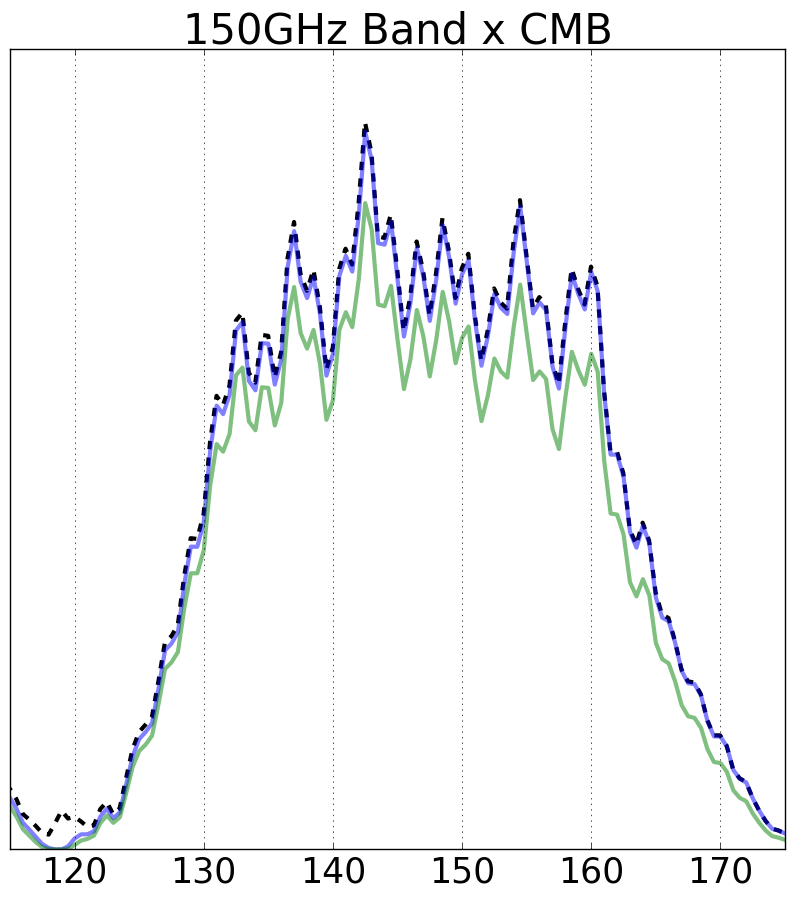
\includegraphics[width=.2\linewidth]{minmax_totals_150GHz_cmb.png}}
 \hspace{-2.5mm} 
 \subfloat{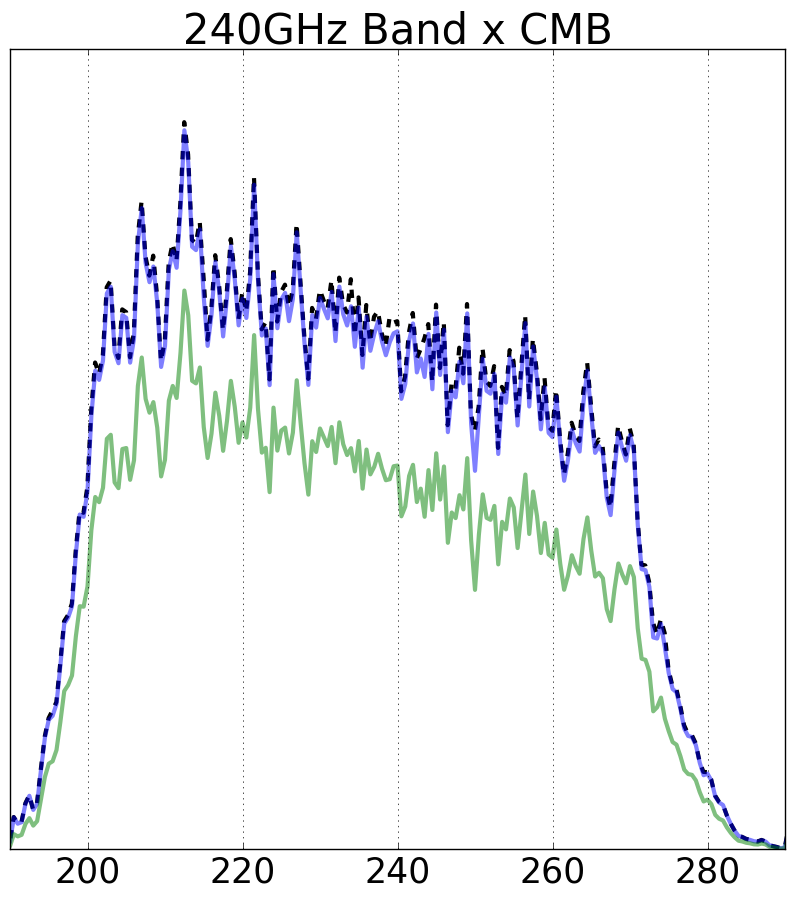
\includegraphics[width=.2\linewidth]{minmax_totals_240GHz_cmb.png}}
 \end{varwidth}
\caption{Minimum and maximum effects of the atmosphere for each of the five simulated frequency bands.  The top row shows the instrument band, the middle row shows band x dust, and the bottom row shows band x CMB.  The blue represents the minimum effect, the green represents the maximum effect, and the black dashed line shows the original band as measured by the FTS.  The y-axis of the plots goes from zero to one and represents the normalized transmission of the band, while the x-axis is the frequency in gigahertz.}
\label{minmax_bands}
\end{figure}

\FloatBarrier

\paragraph{Parameterization:}
Once all combinations of bands and transmission values are generated, the integrated power and band centers are solved for in each case.  To quantify the changes, we calculate the percent difference in the band gain and central frequency from the FTS measured band.  Tables \ref{minmax_gain} and \ref{minmax_center} outline the simulated changes in band gain and centers.  

\begin{table}[h]
 %\parbox{.25\linewidth}{
 \centering
 \resizebox{.5\linewidth}{!}{%
 \begin{tabular}{|c|l l|l l|l l|}
  \hline
  \multicolumn{7}{|c|}{Min and Max Percent Changes - Band Gain} \\
  \hline
  \multirow{3}{*}{Band} 
      & \multicolumn{2}{c|}{Band}
          & \multicolumn{2}{c|}{Dust}
              &\multicolumn{2}{c|}{CMB}\\             \cline{1-7}
  & Min & Max & Min & Max & Min & Max \\  \hline
   20GHz & 0.73\% & 3.22\% & 1.00\% & 4.08\% & 0.88\% & 3.77\% \\      
   40GHz & 4.24\% & 7.47\% & 5.83\% & 9.71\% & 5.07\% & 8.66\% \\      
   90GHz & 3.19\% & 8.98\% & 3.32\% & 9.35\% & 3.20\% & 9.04\% \\      
   150GHz & 1.41\% & 12.8\% & 1.33\% & 13.3\% & 1.40\% & 12.8\% \\      
   240GHz & 1.77\% & 27.8\% & 1.86\% & 28.6\% & 1.73\% & 27.45\% \\      \hline
 \end{tabular}}
\caption{Estimated minimum and maximum percent changes in band gain over a full observing season.}
\label{minmax_gain}
%}
%\hfill
%\parbox{.25\linewidth}{
\end{table}


\begin{table}
 \centering
 \resizebox{.5\linewidth}{!}{%
 \begin{tabular}{|c|l l|l l|l l|}
  \hline
  \multicolumn{7}{|c|}{Min and Max Percent Changes - Band Center} \\
  \hline
  \multirow{3}{*}{Band} 
      & \multicolumn{2}{c|}{Band}
          & \multicolumn{2}{c|}{Dust}
              &\multicolumn{2}{c|}{CMB}\\             \cline{1-7}
  & Min & Max & Min & Max & Min & Max \\  \hline
   20GHz & 0.03\% & 0.26\% & 0.07\% & 0.23\% & 0.05\% & 0.25\% \\      
   40GHz & 0.51\% & 0.78\% & 0.61\% & 0.89\% & 0.57\% & 0.85\% \\      
   90GHz & 0.01\% & 0.10\% & 0.08\% & 0.19\% & 0.03\% & 0.13\% \\      
   150GHz & -0.04\% & 0.20\% & -0.03\% & 0.24\% & -0.04\% & 0.20\% \\      
   240GHz & 0.02\% & 0.36\% & 0.02\% & 0.39\% & 0.02\% & 0.33\% \\      \hline
 \end{tabular}}
\caption{Estimated minimum and maximum percent changes in band center over a full observing season.}
\label{minmax_center}
%}
\end{table}

\FloatBarrier


\section{Polarization Modulators}
A Half Wave Plate (HWP) is an optical device that introduces a phase delay between the two orthogonal polarizations of the incoming signal. It can be made of birifringent crystals (e.g. Sapphire) or metamaterials. The HWP flips the polarization of incoming light along the fast axis of the crystal resulting in a polarization shift of $2\chi$, where $\chi$ is the incoming polarization angle of the light with respect to the fast axis. Thus, a HWP rotating with frequency $f$ mo\-du\-la\-tes the incoming polarization at $2f$, which is detected in the bolometer timestreams at $4f$. The demodulation process described below summarizes the formalism defined in Kusaka \& Essinger-Hileman et al., 2014~\cite{ABS_HWP}.

The detector timestream $d_{m}$ is composed of the unpolarized sky intensity $I$, the modulated polarization signal $P(\chi)$, white noise $N_{w}$, and spurious modulation signals $A(\chi)$ that depend on the HWP angle $\chi$ such that
\begin{equation}
d_{m}= I + P(\chi)+ N_{w} + A(\chi).
\end{equation}
The modulated polarization signal can be represented in terms of the Stokes $Q$ and $U$ parameters, eq.~(\ref{eqn:Stokes})), as
\begin{equation}
P(\chi)=\epsilon \mathrm{Re}\{(Q+iU) m(\chi)\},
\end{equation}
where the modulation is given by $m(\chi)=\exp[-4 i \chi]$ and $\epsilon$ is the polarization modulation efficiency factor, which is close to one. The spurious modulation signals $A(\chi)$ consist of components at every harmonic $n$ of the HWP rotation frequency and can be decomposed into cosine and sine components as
\begin{equation}\label{eqn:achi}
A(\chi)= \sum_{n} A_n(\chi)=\sum_{n}\Big[ (A^{nc}_{0} + \lambda^{nc} I) \cos(n\chi) + (A^{ns}_{0} + \lambda^{ns} I) \sin(n\chi)    \Big].
\end{equation}
Here the $A_{0}$ terms are stable and independent of the sky intensity and the $\lambda$ terms are small~\cite{ABS_HWP}.

The demodulated timestream is, then, extracted by applying a bandpass filter to $d_{m}$ to account for the slight variations in $f$, multiplying $d_{m}$ by $m^*(\chi)$, and applying a low-pass filter that passes $f\lesssim2$~Hz to eliminate higher order terms and all $A^{nc,s}$ and $\lambda^{nc,s}$ terms other than the $n=4$ components. From~\cite{ABS_HWP}, the final demodulated timestream $d_{\bar{d}}$ is then given by
\begin{equation}
d_{\bar{d}}=\frac{1}{2}\Big(\epsilon Q + A^{4c}_{0} + \lambda^{4c} I \Big) + N^{\mathrm{Re}}_{w} + \frac{i}{2}\Big(\epsilon U + A^{4s}_{0} + \lambda^{4s} I \Big) + iN^{\mathrm{Im}}_{w}.
\end{equation}

The optical action of a single layer birifringent material or achromatic metamaterial HWP can be described by the Mueller matrix:
\begin{equation}
M=\begin{bmatrix}
   t  &\rho  &0  &0\\
   \rho  &t  &0  &0\\
   0  &0  &c  &-s\\
   0  &0  &s  &c
\end{bmatrix}.
\label{eq:Mueller_Matrix}
\end{equation}

The $t$ term is proportional to the total unpolarized intensity transmitted by the HWP, the $\rho$ term to the differential transmission of the HWP. The $c$ and $s$ terms are responsible for the modulation of the polarized components, the $\rho$ term for the unpolarized ones. For an ideal HWP: $t=1$, $\rho=0$, $c=-1$, $s=0$. Deviations from these values are due, e.g., to the spectral behavior of the birifringent material/metamaterial (as we will deeply investigate in the next sections). The left panel of Fig.~\ref{fig:Mueller_elements} shows the Mueller matrix elements $M_{ij}$ for a single-layer HWP as a function of the frequency of the incoming radiation. 

\begin{figure}
\begin{center}
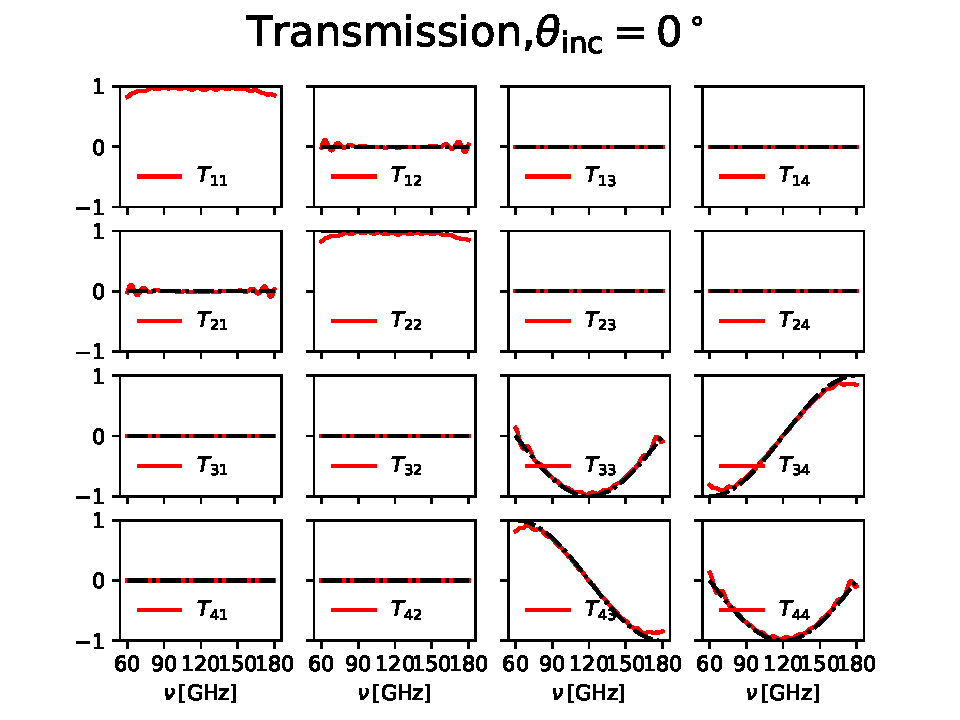
\includegraphics[0.5\linewidth]{plot/1layer_AHWP_120.pdf}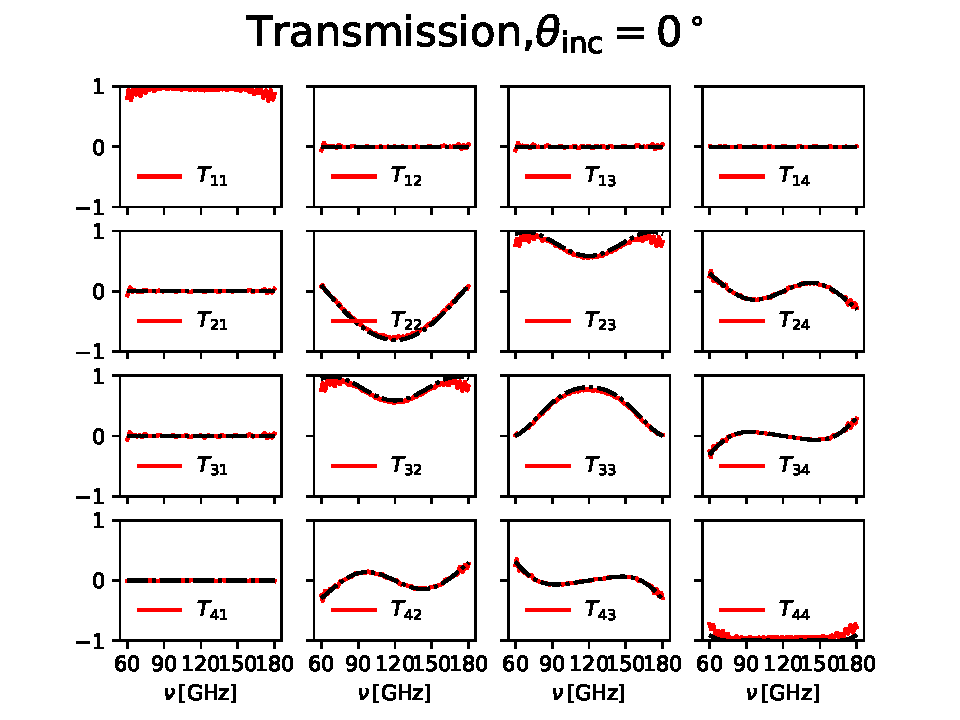
\includegraphics[0.5\linewidth]{plot/3layer_AHWP_120.pdf}
\end{center}
\caption{Mueller matrix elements $M_{ij}$ for a single-layer HWP (left panel) and a three-layer AHWP (right panel) as a function of the frequency of the incident radiation. Each layer is a made of Sapphire crystal and it is optimized for a central frequency of $120\,\mathrm{GHz}$. The AHWP is optimized to cover the broad-band range including the $90\,\mathrm{GHz}$ and $150\,\mathrm{GHz}$ frequency bands. The behaviour of $M_{ij}$ with the frequency for the single-layer HWP agrees with the description in eq.~(\ref{eq:Mueller_Matrix}). The behaviour of $M_{ij}$ for the AHWP is more complicated and agrees with the combination of three Mueller matrices as in eq.~(\ref{eq:Mueller_Matrix}) and rotated with respect to each other. Further details are provided in Sec.~\ref{subsec:modeff}. In both panels, the black dashed-dotted lines correspond to the elements of an ideal HWP.}\label{fig:Mueller_elements}
\end{figure}

For an achromatic HWP, made of stacks of birifringent material, the Mueller matrix presents further non-zero terms with respect to the ones in eq.\,(\ref{eq:Mueller_Matrix}), see Sec.\,\ref{subsec:modeff}. The right panel of Fig.~\ref{fig:Mueller_elements} shows the Mueller matrix elements $M_{ij}$ for a three-layer AHWP as a function of the frequency of the incoming radiation. The presence of additional non-zero elements with respect to the single-layer HWP is clearly visible. 

The HWP optical action creates a non zero $c$ and $s$ terms. Because this does not depend on the direction of the incoming radiation (upwards or downwards), the HWP Mueller matrix has the same shape, eq.\,(\ref{eq:Mueller_Matrix}), both in transmission and in reflection; the value of the corresponding Mueller matrix components changes according to the amplitudes of the electric field transmitted and reflected by the HWP.









\subsection{Slant Incident HWP properties}

\paragraph{Description:}
At non-normal incidence, the HWP optical properties change. This effect is small for angles $<$10 degrees away from the normal incidence and increases for larger angular deviations. Stray light, instrumental emissions and reflections can produce off-axis radiation crossing and reflecting the HWP.

\textbf{What systematics do these contribute to?} The general result of slant incidence effects is to change the phase delay and the amplitude of the 2$\,f$ and 4$\,f$ signals; any approach consisting in measuring/estimating these signals under normal incidence hypothesis and subtract from the data as template, might not be reliable. 

\subsubsection{Birefringent HWP}\label{slant_biri}

\paragraph{Plan to model and/or measure:}
For a birefringent HWP, how the optical properties change with the incidence angle can be modeled if you know the optical properties of the birefringent material as a function of frequency and include the AR coating. This can be estimated with numerical simulations and crystallography properties. Fourier Trasform Spectrometer (FTS) and reflectometery measurements with the angle of incoming light at different, non-normal, incident angles with respect to the HWP can be used to measure the dependence of the optical properties as a function of the incident angle.

\textbf{Using the modeled/measured values, how do we model the impact of this response on the science?}
These measurements can be used to build the Mueller matrix under slant incident incoming radiation. Fig.~\ref{fig:Sa_elements} shows the Mueller matrix elements $M_{ij}$ in transmission of a single-layer HWP optimized for $150\,\mathrm{GHz}$. The behaviour of the elements is shown as a function of the HWP rotation angle $\chi$ in the case of normal incidence (blue curve), at $10^\circ$-incidence (orange) and at $20^\circ$-incidence (green). To highlight the small deviation of slant incidence from the case of normal incidence, the right panel of Fig.~\ref{fig:Sa_elements} reports the difference between $M_{ij}$ at slant incidence and $M_{ij}$ at normal incidence.  

An alternative approach to model the behaviuor at slant incidence would be to directly measure the HWP Mueller matrix components studying the output signal from an unpolarized and totally polarized incoming radiation crossing the HWP and followed by a fixed polarizer. The measurement should be performed for dfferent frequency values, to reconstruct the spectral trend of the components: see for example Figs.\,5 and 6 in \cite{Salatino17} which demonstrate how these trends change with respect to the incidence angle of the incoming radiation. The simulated trend of Fig.\,5 in \cite{Salatino17} agrees well with the ones measured from the Spider HWP \cite{Bryan10}.


This effect is not modeled in the literature, and could be large in some cases, so the SRF is 4.

\paragraph{Uncertainty/Range:}
In most cases the optical properties (refraction indices, absorption angle) come from literature, so there is some uncertainty in the parameters from the variation between batches of materials. However, the main source of uncertainty comes from uncertainty in understanding how these optical properties, generally measured at room temperature, scale to cryogenic temperatures.

\textbf{Include how big the science impacts can be for this within SO.}

\paragraph{Parameterization:}
Analytically, this effect can be estimated building the Mueller matrix of the birifringent HWP considering how the refraction index along the extraordinary axis depends on the incidence angle, $i$:
\begin{equation}
%n(i)=((\frac{\cos{i}}{n_e(\nu))^2}+(\frac{\sin{i}}{n_o(\nu)})^2)^{(-0.5)};
n(i)=n_e\sqrt{1+(n_e^{-2}(\nu)-n_o^{-2}(\nu))n_1^2\sin^2(i)\cos^2(\chi)};
\end{equation}
where $n_e(\nu)$ ($n_o(\nu)$) are the extraordinary (ordinary) refraction index, $\nu$ is the frequency of the incoming radiation, $n_1$ is the index of refraction of the medium where the incoming radiation propagates ($n_1=1$ as we usually assume air), and $\chi$ is the HWP rotation angle. \textbf{How do we parametrize the science impact}

From both the analytical approach and the experimental one (i.e. reconstruction of the Mueller matrix components from the measurement described above), the amplitude of the resulting 2$\,f$ and 4$\,f$ signals, i.e. $A_2$ and $A_4$, can be estimated as:

\begin{eqnarray}
  A_2 &=& \int_{\Delta\nu} \frac{I(\nu)+Q(\nu)}{2} \rho(\nu) d\nu\\ \label{A2}
  A_4 &=& \int_{\Delta\nu} \frac{t(\nu)-c(\nu)}{4} Q(\nu) d\nu; \label{A4}
\end{eqnarray}
where $I(\nu)$ and $Q(\nu)$ is the Stokes vector of the incoming radiation (here as an example we assumed to be $(I(\nu), Q(\nu),0,0)$),
$\rho(\nu), t(\nu)$ and $c(\nu)$ the Mueller matrix components (eq.\,\ref{eq:Mueller_Matrix}). The spectral trend of all the involved quantities is integrated on a given HWP band $\Delta\nu$. A more generic approach to quantify the coefficients $A_2$ and $A_4$ is detailed in Sec.~\ref{IP downstream of HWP}.

\begin{figure}
\centering
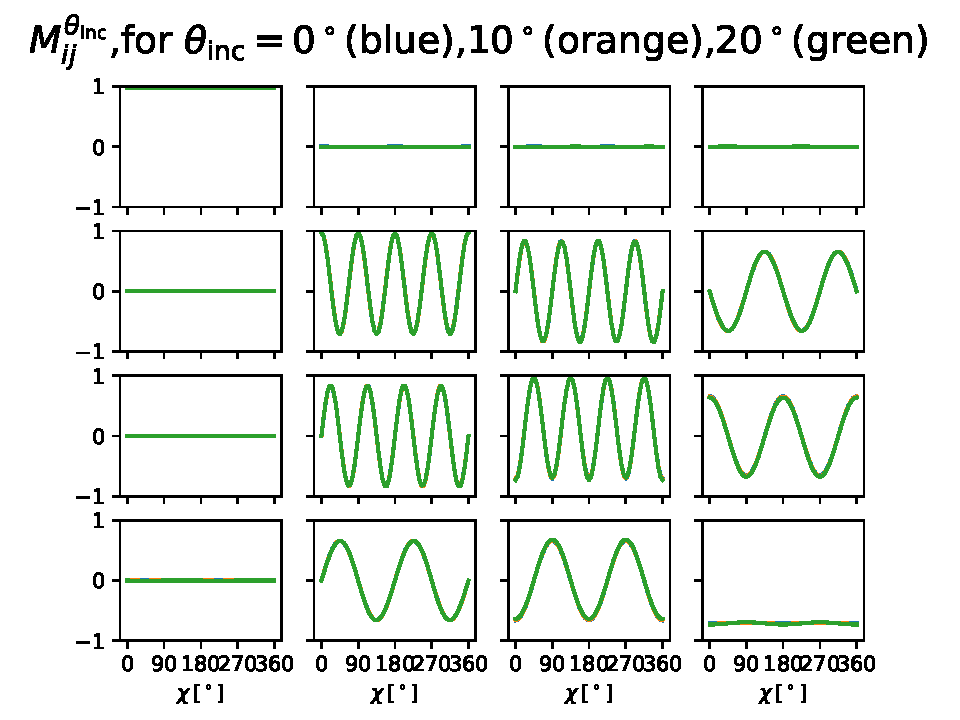
\includegraphics[width=0.5\linewidth]{figures/Mueller_elements_0_10_20deg.pdf}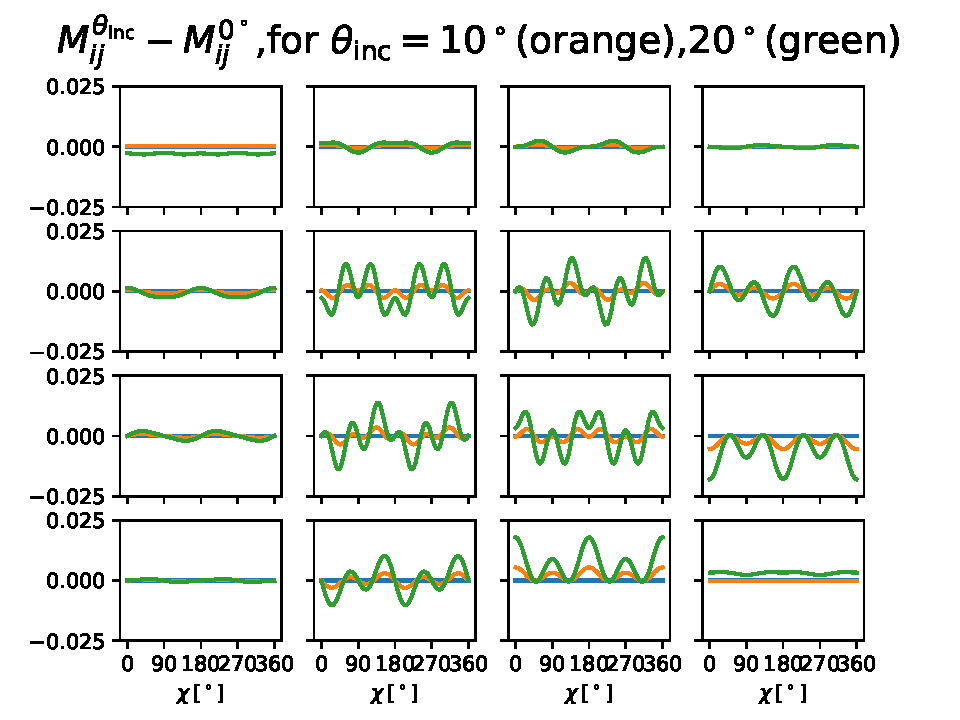
\includegraphics[width=0.5\linewidth]{figures/Mueller_elements_diff_1l.pdf}
\caption{Left panel: Mueller matrix components $M_{ij}$ in transmission as a function of the HWP rotation angle $\chi$. The components are for a real Sapphire HWP
optimized for 120 GHz (with AR coating). We have considered three incidence angles: $\theta_\mathrm{inc}=0^\circ$ (blue), $\theta_\mathrm{inc}=10^\circ$ (orange), and $\theta_\mathrm{inc}=20^\circ$ (green). Right panel: To highlight the small deviation of the behaviour of the HWP from the case of normal incidence, the difference between Mueller matrix components at non-normal incidence and the Mueller matrix components at $0^\circ$-incidence are shown as a function of the rotation angle $\chi$.
}\label{fig:Sa_elements}
\end{figure}

%\begin{figure}
%\centering
%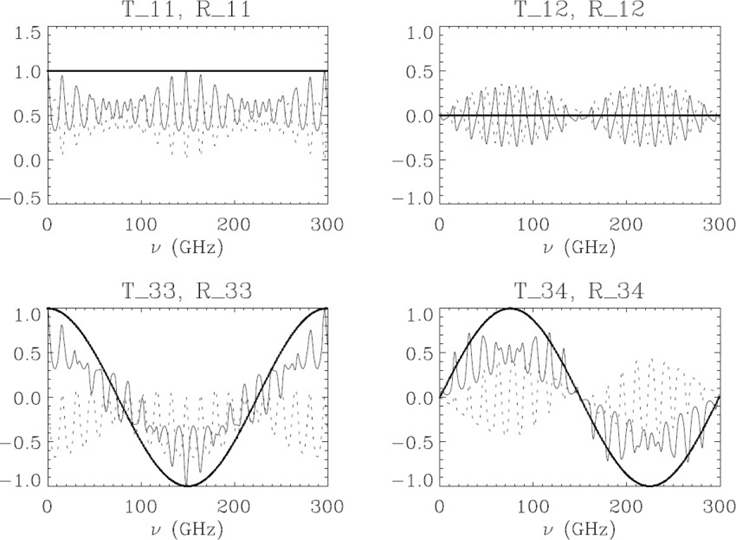
\includegraphics[width=0.6\linewidth]{figures/0deg.png}
%\caption{Mueller matrix components, for both transmission (T) and reflection (R), of a real Sapphire HWP
%optimized for 150 GHz (no AR coating). The incoming radiation is at normal incidence \cite{Salatino17}.
%}\label{0deg}
%\end{figure}

%\begin{figure}
%\centering
%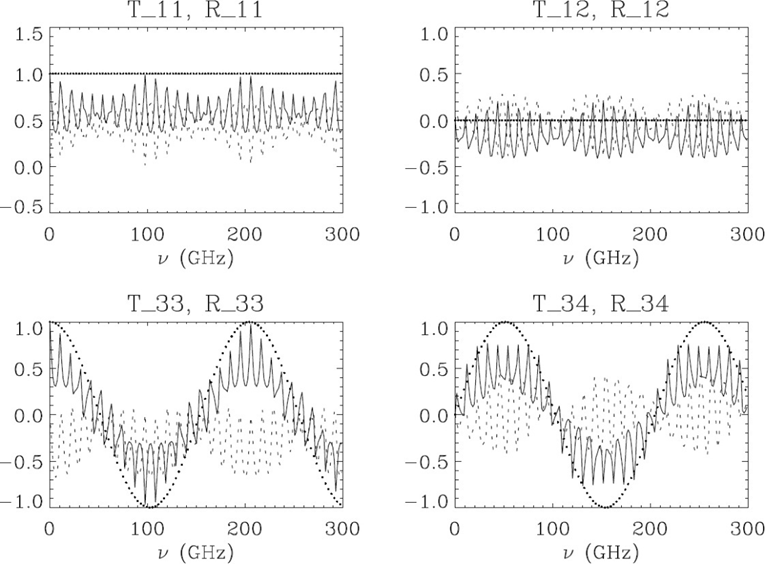
\includegraphics[width=0.6\linewidth]{figures/45deg.png}
%\caption{Mueller matrix components, for both transmission (T) and reflection (R), of a real Sapphire HWP
%optimized for 150 GHz (no AR coating). The incoming radiation is at 45deg incidence \cite{Salatino17}.}\label{45deg}
%\end{figure}

%------------------------
\subsubsection{Metamaterial HWP}

\begin{figure}
\centering
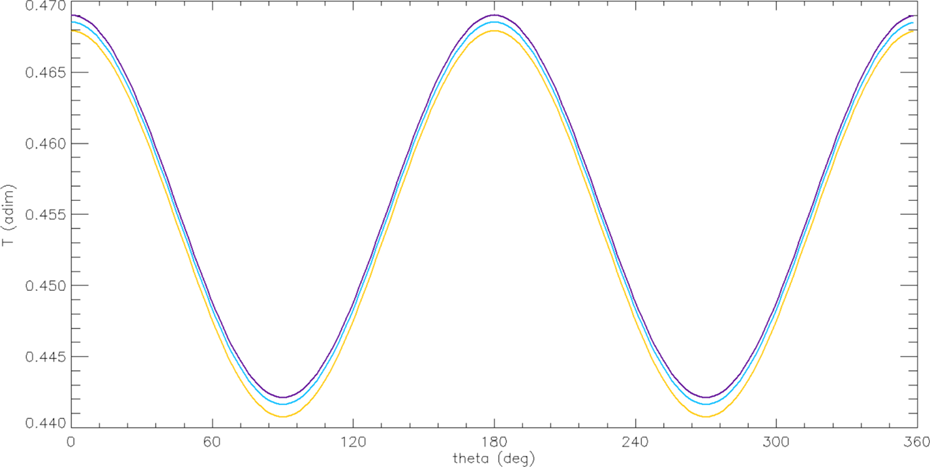
\includegraphics[width=0.6\linewidth]{figures/meta1.png}
\caption{Simulated output signal (dimensionless units) at 70GHz from an unpolarized radiation crossing the AdvACT MF metamaterial HWP. The HWP is %optimized for a frequency band centered
on 90 GHz. Violet line: -10deg, cyan line 0deg and orange 10deg incident angle. At 10deg away from the normal incidence, the output %signal
changes by 0.03.}\label{meta1}
\end{figure}

\begin{figure}
\centering
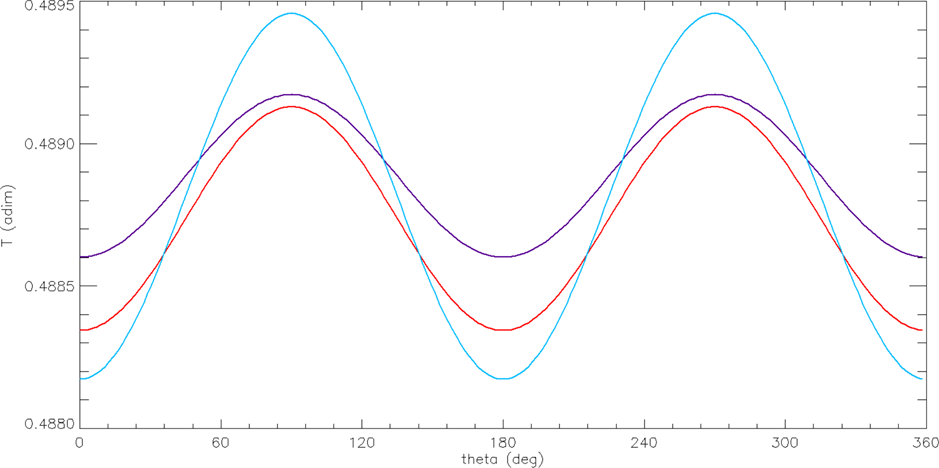
\includegraphics[width=0.6\linewidth]{figures/meta2.png}
\caption{Simulated output signal (dimensionless units) at 90GHz from an unpolarized radiation crossing the AdvACT MF metamaterial HWP. The HWP is %optimized for a frequency band centered
on 90 GHz. Violet line: -10deg, red line 0deg and cyan 10deg incident angle. At 10deg away from the normal incidence, the output signal
changes by 0.0015.}\label{meta2}
\end{figure}

\paragraph{Plan to model and/or measure:}
For a metamaterial HWP, uderstanding of how the optical properties change with the incident angle requires simulations in HFSS or CST. HFSS simulations have demonstrated that the variation in the output signal increases at frequencies closest to the central working frequency of the
HWP (Figs. \ref{meta1} and \ref{meta2}). 
Like the birefringent case, FTS and reflectometry measurements can provide experimental estimates of the optical properties.

\textbf{Using the modeled/measured values, how do we model the impact of this response on the science?}

This effect is not modeled in the literature, and could be large in some cases, so the SRF is 4.

\paragraph{Uncertainty/Range:}
\textbf{Add info here as it becomes available.}

\paragraph{Parameterization:}
HFSS/CST simulations can give the optical properties as a function of the incident angle $i$. \textbf{How do we parametrize the science impact} From these, the Mueller matrix for slant incident angle can be build and the amplitude of the $2\,f$ and $4\,f$ signals estimated as described for the birifringent HWP (Sec.\,\ref{slant_biri}). 

% !TEX root =  ../syst_master.tex 

\subsection{Polarization modulation efficiency}\label{subsec:modeff}

\paragraph{Description:}
The polarization modulation efficiency quantifies how much of the incident polarization signal $P_\mathrm{p,in}$ is transmitted by the HWP as $P_\mathrm{p,out}$:
\begin{equation}
\epsilon \def \frac{P_\mathrm{out}}{P_\mathrm{in}}
\end{equation}
in the absence of systematic effects that induce a 2f component.

With the definition above, the total intensity $I_\mathrm{out}$ at the detector can be expressed as~\cite{Matsumura:2008zx}:
\begin{equation}
I_\mathrm{out}=\frac{1}{2}\left[I_\mathrm{in}+\epsilon\sqrt{Q^2+U^2} \cos(4\chi-4\phi)\right]
\end{equation}
where $I_\mathrm{in}$ is the total incoming signal, $\chi$ is the rotation angle of the HWP, and $\phi$ is the frequency-dependent phase offset which is not relevant in the case of a monochromatic HWP.

The modulation efficiency depends on the incident frequency $\nu$, the detector bandwidth $\Delta \nu$, the incoming polarized signal $I_\mathrm{p,in}$, the incidence angle of the incoming radiation $\theta_\mathrm{i}$ and the physical properties of the HWP. In particular, the design of the HWP can be chosen in order to optimize the modulation efficiency over a broad range of frequencies. 

\paragraph{Plan to model and/or measure:}
To model the modulation efficiency, we can compute the analytic expression in the two simple cases of a monochromatic HWP (1 layer) and an achromatic HWP (AHWP, multi-layers) at normal incidence. We make use of the Mueller calculus and represent the HWP stack (arbitrary number of layers, with and without anti-reflection coating) and the detector as Mueller matrices. The Mueller matrix for the single-layer HWP takes the generic form 
\begin{equation} 
\begin{bmatrix}
   T  &\rho  &0  &0\\
   \rho  &T  &0  &0\\
   0  &0  &c  &-s\\
   0  &0  &s  &c
\end{bmatrix}
\end{equation}\label{eq:Mueller_Matrix}
which allows for leakage off-diagonal terms. In the case of the AHWP, Eq.~\ref{eq:Mueller_matrix} takes a different form, accounting for the fact that the AHWP is a stack of several layers rotated by a certain angle with respect to the first layer. Each layer is represented by a Mueller matrix as Eq.~\ref{eq:Mueller_matrix}, and the rotation with respect to the first layer is modelled with the usual rotation matrices $R(\theta)$:
\begin{equation}
R{(2\phi)}\cdot M \cdot R(-2\phi).
\end{equation} 

The elements of the HWP (either monochromatic or achromatic) Mueller matrix are computed following the generalised transfer matrix approach~\cite{Essinger-Hileman_TM}. 

We finally model the global rotation of the HWP stack with the usual rotation matrices:
\begin{equation}
R{(2\chi)}\cdot M_\mathrm{stack} \cdot R(-2\chi).
\end{equation}

The output signal can be then analytically expressed as a series of cosine terms. The modulation efficiency is then computed as~\cite{Hanany:2005vx,Matsumura:2008zx}:
\begin{equation}\label{eq:eff}
\epsilon=\frac{A_4}{A_0}
\end{equation}
where $A_x$ is the coefficient of the n-th harmonic.

In more generic cases, including more complicated configurations, such as multi-layer stacks, slant incidence, and broad-band incident radiation, we compute the output signal at the detector following the Mueller calculus as in the analytic approach, and fit the output signal to an harmonic series of cosine terms:
\begin{equation}
I_\mathrm{out}=\Sigma_{i=0,n} A_i \cos(i\chi-i\phi).
\end{equation}

The modulation efficiency is then computed as in Eq.~\ref{eq:eff}. %\textbf{Missing an equation label somewhere}

Fig.~\ref{fig:eff} shows the polarization modulation efficiency as a function of frequency computed with the fitting procedure in two cases: a single layer HWP (curves peaking at $120\,\mathrm{GHz}$); and a 3-layer AHWP optimized to cover the two bands centered at $90\,\mathrm{GHz}$ and $150\,\mathrm{GHz}$, depicted as the gray vertical bands. It is clear that the multi-layer design is able to provide a nearly maximal polarization modulation efficiency over a broad range of frequencies. 
The different colors correspond to different incidence angles, as detailed in the legend. The modulation efficiency does not change dramatically with the incidence angle.

\begin{figure}
\begin{center}
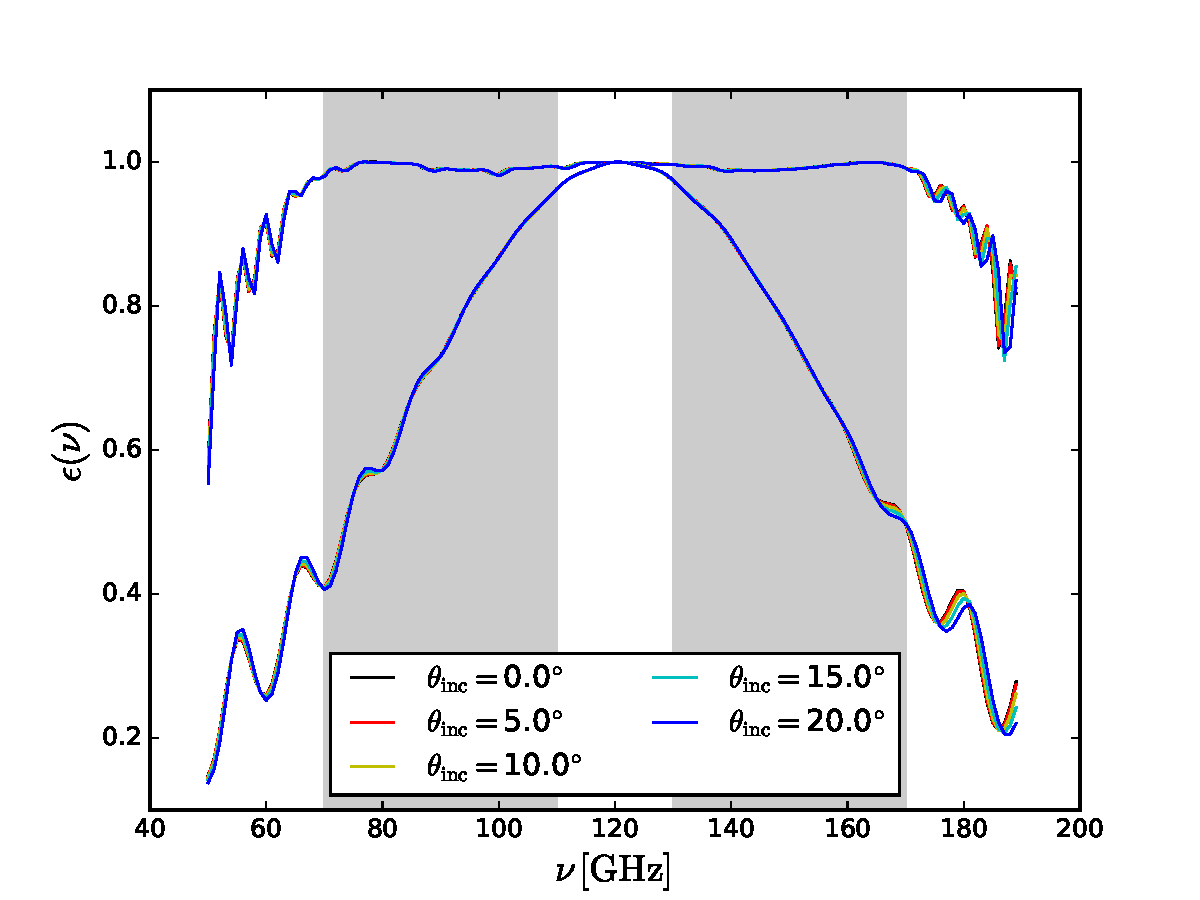
\includegraphics{figures/Eps_vs_nu_3l_PB2.pdf}
\end{center}
\caption{Polarization modulation efficiency as a function of frequency for two HWP designs: a single-layer (monochromatic) HWP centered at $120\,\mathrm{GHZ}$; and a 3-layer AHWP optimized for the two bands at $90\,\mathrm{GHz}$ and $150\,\mathrm{GHz}$. The vertical gray bands identify the two frequency bands. The different colors correspond to different incidence angles of the incoming radiation. There is not a strong dependency on the incidence angle. The assumed thickness and indexes of the sapphire are the same as in Tab.2 of~\cite{PB2a_WHWP}.}\label{fig:eff}
\end{figure}


\paragraph{Uncertainty/Range:}
The systematic effect related to the modulation efficiency is known and can be kept under control, but because it needs to be modeled, its SRF is 3.

The main systematic effect is a suppression of power in polarisation. A low modulation efficiency means that a low fraction of the polarised signal is transmitted through the HWP to the detector. In addition, what we really care about is the behaviour of the modulation efficiency over the frequency band.

For a single-layer HWP, the modulation efficiency is nearly maximal at the central frequency, and decreases rapidly otherwise. The band-averaged modulation efficiency can be therefore quite low, depending on the choice of the bandwidth.

The stacking of multiple layers of birefringent crystals allows to obtain a nearly maximal modulation efficiency over a broader range of frequencies. As an example, Fig.~\ref{fig:eff} shows the difference between a single layer HWP optimized for $120\,\mathrm{GHz}$ and a 3-layer AHWP which is optimized for the two bands at $90\,\mathrm{GHz}$ and $150\,\mathrm{GHz}$. For comparison, the band-averaged modulation efficiency for the single-layer HWP is 72\% over a 30\% frequency band centered at $90\,\mathrm{GHz}$ and 75\% for a 30\% frequency band centered at $150\,\mathrm{GHz}$. The use of a 3-layer AHWP allows to improve those figures up to a 99\% modulation efficiency over both frequency bands.

The final design of the AHWP, and in particular the choice of the number of layers which in turn sets the overall thickness of the stack, has to come as a balance between the increased modulation efficiency and the increased absorption and emission from the thicker stack of multiple layers.
%\textbf{How does this propagate into systematics? At what level does it become significant?}

\paragraph{Parameterization:}
This effect is parameterized as the modulation efficiency as a function of frequency, $\epsilon (\nu)$. The modulation efficiency can be predicted for a given design of the HWP. This prediction gives an estimate of the fraction of polarized signal that is transmitted from the HWP to the detector, or the next element in the optical chain.


%\textbf{Cite these in the text and put the references in the bibliography file}
%
%\paragraph{References:}
%The description of this systematic entry is based on the following references:
%\begin{itemize}
%\item T. Hessinger-Hileman, ``Transfer matrix for treating stratified media including birefringent crystals'', arXiv:1301.6160v3 [physics.optics], for the modelling of the HWP
%\item T. Matsumura \textit{et al}, ``Analysis of performance of three- and five-stack achromatic half-wave plates at millimeter wavelengths'', arXiv:0806.1518v1 [physics.optics], for the definition and calculation methods of $\epsilon$.
%\item S. Hanany \textit{et al}, ``A Millimeter-Wave Achromatic Half Wave Plate'', arXiv:physics/0503122 [physics.optics], for the definition and calculation of $\epsilon$ according to the fitting procedure.
%\end{itemize}

\subsection{Polarization Angle Frequency Dependence of HWP}

\paragraph{Description:}
%Description of systematic effect, including relevant equations and
%parameterization for TWGs. Note that each variable in each equation should be
%defined. This should include where we expect to get the value of this variable
%from (TWG, literature, etc.)

We define polarization angle as the angle betweeen the light and the HWP, with incident light being rotated by the HWP to a different, transmitted angle. This polarization angle has a dependence on the frequency of light, as well as the optical properties.

A strategy to mitigate this systematics has been proposed in \cite{Matsumura14}. It consists of an additional, stationary HWP behind the rotating one. This counteracts the frequency polarization angle dependence while maintaining broadband polarization modulation. 

\paragraph{Plan to model and/or measure:}
%Plan to model/measure effect. Use TRLs to describe how well we understand/can model the effect.
A Muller Matrix paramaterization should be sufficient to model this effect, although it also could be modeled using a full transmission line model.  The transmission line model may more accuratly capture the behavior since it takes the multiple reflections between the various layers into account.

For a silicon metamaterial HWP, the phase shifter and its AR can be modeled in HFSS; this depenendence can be easily derived from the simulation.

Several HWP are available inside the Simons Observatory collaboration that can be used in laboratory to measure this effect, such as by using a vector network analyzer set up.

\paragraph{Uncertainty/Range:}
%This section should include the uncertainty of
%known parameters and/or the expected range of parameters for consideration
Discussion in \cite{Matsumura09} show this can be up to about 20 degrees for some HWPs.




\paragraph{Parameterization:}
%This section should include the parameterization of figures of
%merit and the output to the SWGs.

As discussed in \cite{Matsumura09}, a Muller Matrix representation of the HWP stack can give the frequency dependence of the polarization angle effectively.



\subsection{HWP $I\rightarrow P$}
\label{IP downstream of HWP}
\paragraph{Description:}
When passing through the HWP, incoming polarized radiation is rotated by $2\chi$, where $\chi$ is the rotation angle of the HWP optical axis. The signal is finally seen by the detectors at $4\chi$. Any unpolarized signal which is modulated at $4\chi$ represents a source of systematics. A list of possible sources of spurious $4\chi$ signals can be found in Sec.\,III of~\cite{Kusaka_ABS}. The main source comes from non-normal incidence, since the reflected signal by the crystal itself and the AR coating is partly polarised and thus modulated by $4\chi$. Other sources include polarized emission due to differential transmission and differential absorption. Although these emission is usually modulated at $2\chi$, it might be further modulated at $4\chi$ due to HWP misalignment and/or non uniform AR coating.

\paragraph{Plan to model and/or measure:}
We expect the $I\rightarrow P$ leakage to be small. Nevertheless, it needs to be carefully modelled and understood, as the major unpolarised sources (emissivity from warm optical elements in the optical chain, atmospheric noise and unpolarised CMB) are many order of magnitudes higher than the actual signal of interest, the CMB polarization signal. For these reasones, the SRF is 4.

In order to model this effect, we need the global unpolarized power incident on the sky-side of the HWP, the HWP physical properties as well as the proprties of any AR coating, and a mapping between the incidence angle of the incoming radiation and the position on focal plane where the incoming radiation is going to be collected. 

We model the incoming and outgoing signals, the HWP and the detectors following the Mueller matrix approach. We make use of the transfer matrix formalism to model the Mueller matrix for the HWP and AR coating stack~\cite{Essinger-Hileman_TM}. In the case of the SAC, the incoming radiation can be represented as a plane wave. Therefore, at each incidence angle roughly corresponds a specific position on the focal plane where the signal is focused and collected. The mapping between the incidence angle and the position on the focal plane should be accurately modelled through ray-tracing techniques. However, a first estimate can be obtained by assuming a simple relation, such as 
\begin{equation}\label{eq:fp}
\delta x= f \delta \theta,
\end{equation}
where $\delta x$ is the distance on the focal plane with respect to the central pixel, $\delta \theta$ is the angular distance with respect to normal incidence, and $f$ represents the scaling coefficient between $\theta$ and $x$ (a good approximation for $f$ is $f\simeq 1\,\mathrm{cm\,deg^{-1}}$).

To predict the magnitude of the effect, we assume that unpolarised signal passes through the HWP at a generic incidence angle $\theta$. We compute the output signal as a function of the rotation angle $\chi$ of the HWP. We fit this signal with a harmonic series of cosine terms and isolate the coefficient $A_4$ of the $4\chi$ component. This represents our estimate of $I\rightarrow P$ leakage. This calcuation is done for different incidence angles $\theta$. The set of $A_4$ coefficients as a function of $\theta$ is then assigned a position on the focal plane according to eq.~(\ref{eq:fp}).

\paragraph{Uncertainty/Range:}
An example of $I\rightarrow P$ leakage estimated following the approach above is shown in Fig.~\ref{fig:ip_fp}. The figure shows the normalized $A_4$ component as collected on the focal plane, coming from an incoming unpolarized radiation which passes through the HWP. The HWP is achromatic and optimized to cover both the $90\,\mathrm{GHz}$ and $150\,\mathrm{GHz}$ bands. As expected, the $I\rightarrow P$ leakage is small, lower than 0.02\%. As also expected, the higher contribution is relegated to the edges of the focal plane, as it comes from the largest incidence angles $\theta\sim 20^\circ$.

\begin{figure}
\begin{center}
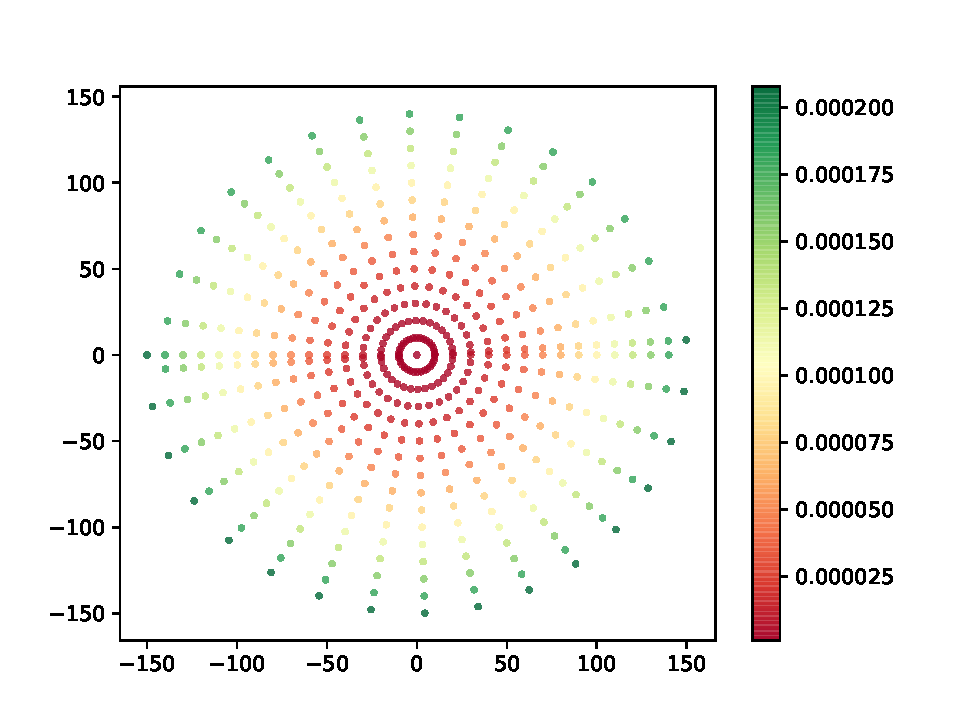
\includegraphics{figures/A4_focalPlane.pdf}
\end{center}
\caption{Normalized $A_4$ component as collected on the focal plane, coming from an incoming unpolarized radiation which passes through the HWP. The incidence angles are in the range $[-20^\circ,20^\circ]$. The relation between the incidence angle and the position on the focal plane is given in eq.~(\ref{eq:fp}). The HWP is achromatic and optimized to cover both the $90\,\mathrm{GHz}$ and $150\,\mathrm{GHz}$ bands. The assumed thickness and indexes of the sapphire are the same as in Tab.\,2 of~\cite{PB2a_WHWP}.}\label{fig:ip_fp}
\end{figure}

\paragraph{Parameterization:}
The $I\rightarrow P$ leakage can be parametrized as the coefficient of the 4-th harmonic in the series expansion used to parametrize the output signal as transmitted by the HWP. This coefficient can be estimated as a function of the incidence angle and then assigned to a position on the focal plane. This last assignment requires ray-tracing techniques and therefore knowledge of the optical chain. However, a quick estimate can be done by assuming a simple relation between incidence angle and position on the focal plane, especially in the case of SAC.

\subsection{Thermal Variation in HWP Temperature}

\paragraph{Description:}
In practice, the HWP has thermal gradients and fluctuations. A non-uniform HWP temperature and its temporal fluctuations create spatial and time dependent 0$f$, 1$f$, 2$f$, and 4$f$ signals that depend on the amplitude of the harmonic decomposition of the temperature profile of the HWP. 

\textbf{Add a few sentences about how estimating the HWP template wrong because it is spatially and temporally varying can translate into leakage.}

\paragraph{Plan to model and/or measure:}
To model this effect, we can use a thermal finite element analysis of a HWP thermalized with a suitable heat sink and with realistic time variable loading. \textbf{How can we estimate the next step (the impact on leakage from this)?}
To measure this, we can use cryogenic measurements of the thermal gradients, and on-sky measurements of polarization leakage will include this effect (as well as other instrumental sources)

This effect is expected to be subdominant, so the SRF is 3.


\paragraph{Uncertainty/Range:}
The uncertainties in these models will be limited by how realistic models of the time variation of the loading are. For a sapphire HWP, we expect the time variation effect to be small, as sapphire has a large thermal conductivity and large heat capacity, giving it both good thermalization properties and a large time constant.
 \textbf{Add more detail if we model this.}

\paragraph{Parameterization:}
We can parameterize this using the HWP thermal fluctuations: $\Delta_{HWP}(x,y,t)$ with $(x,y)$ the spatial coordinates of the HWP and $t$ the time and the effect on the HWP thermal fluctuation time constant: 

\begin{equation}
\tau_{T_{HWP}} = C(T_{HWP})/G(T_{HWP}, T_{BCK})
\end{equation}

where $C$ is the HWP heat capacity as a function of its temperatue $T_{HWP}$, and $G$ is the thermal link between the HWP at $T_{HWP}$ and the surrounding environment at $T_{BCK}$. 

Using this, we expect the HWP temperature to fluctuate, assuming a fluctuating background at frequency $\omega_{BCK}$, as

 \begin{equation} 
 T_{HWP} \propto \frac{e^{i \omega_{BCK} t}}{i \omega_{BCK} + 1/\tau_{T_{HWP}}}
 \end{equation}
 
 Because the time constant is large, we expect the thermal fluctuation to manifest at very low frequencies $\omega_{BCK}$. To estimate the scientific impact, we could parameterize this with spatially and temporally varying HWP template values.

% !TEX root =  ../syst_master.tex 

\subsection{Differential Optical Properties of a HWP}
\label{HWP Differential Optical Properties}

\paragraph{Description:}
Because the HWP is birefringent, the HWP has different transmission coefficients along the fast and slow axes of the crystal,
which produces differential absorption and emission coefficients along the two axes. Because of this, transmitted unpolarized light and emitted light both are partially polarized by the HWP. The polarization direction rotates with the HWP, so this signal couples to the detectors at 2$f$. While the science band is at $4f$, the $2f$ signal can leak into the $4f$ signal through... \textbf{fill this out a bit}.

\paragraph{Plan to model and/or measure:}
To model this effect, we require the HWP Mueller matrix and information about the optical filter chain. Knowing the temperatures, efficiencies, and emissivities of each component in the optical chain,
the unpolarized power can be propagated through each element to find the incident unpolarized power on the HWP.
If $P_n$ is the unpolarized power crossing the $n^\text{th}$ element, $\eta_n$ the efficiency, $\varepsilon_n$ the emissivity, and $B$ the spectral brightness, given the temperature $T_n$,
the propagation step is 
\begin{equation}
\label{unpolarized_propagation}
P_{n+1}(\nu) = \eta_n(\nu) P_n(\nu) + \varepsilon_n(\nu) A\Omega(\nu)\;  B(\nu, T_n) .
\end{equation}


The HWP Mueller matrix (Equation~\ref{eq:Mueller_Matrix} is calculated using the method described in \cite{Salatino16}, where all elements are dependent on frequency, incident angle and spatial position (x,y). The $\rho$ components represent the differential transmission of the HWP. While the polarized fraction of the transmitted and emitted light are equal and opposite, they do not cancel because the radiation sources are at different temperatures.
If we define $P_\text{HWP}$ to be the incident power on the HWP, the polarized power output is 
\begin{equation}
\label{eq:polarized_output}
P_\text{HWP + 1}(\nu) = \rho(\nu)(P_\text{HWP} - A\Omega(\nu)B(\nu, T_\text{HWP})),
\end{equation}
with $A_2 = \rho$. 

If we define $\eta_\text{det}$ to be the combined efficiency of all elements after the HWP,
the final 2$f$ signal produced by the HWP is 
\[
A^{(2)} = \int_{\nu_\text{low}}^{\nu_\text{high}} \eta(\nu) P_\text{HWP + 1}(\nu) d\nu.
\]

\textbf{How do we model how much leaks into $4f$ frmo $2f$?}

Since this effect can leak into the science band, it is important to model and thus has an SRF of 3.
\paragraph{Uncertainty/Range:}
For 145 GHz, this method gives values of $a_2 = .35\%$, and a value of 
$A^{(2)} = .0165 \text{pW} = 238 \text{mK}_\text{CMB}$. 
\textbf{We expect similar values for similar frequency values}.
\textbf{Describe how much of this leaks into $4f$ and contaminates our actual science signal.}

\paragraph{Parameterization:}
We require $T$ and $\rho$ from the HWP Mueller matrix\cite{Salatino16}, and an optical chain input file containing
absorption, temperature, and spill/scatter/reflection coefficients for each element. The Mueller matrix components can be theoretically estimated by transfer matrix model \cite{Essinger-Hileman13} or HFSS simulations. They can be experimentally measured with FTS measurements. We parameterize this with the $A_2$ component of the HWP template and a leakage coefficienct ($\epsilon_{2,4}$) between $2f$ and $4f$.


% !TEX root =  ../syst_master.tex 

\subsection{$I\rightarrow P$ leakage and Instrumental Polarization upstream of the HWP}
\label{IP upstream of HWP}

\paragraph{Description:}
Any polarized signal originating from the telescope upstream of the HWP will be rotated and coupled to the detector at 4$f$,
making it indistinguishable from the sky polarization.
This includes the intensity dependent $I\rightarrow P$ leakage, 
described and calculated in section \ref{instrumental_polarization} 
along with polarized emission from optical elements. 

The IP coefficient and polarized emissivity are both caused by different transmission coefficients along orthogonal axes,
and are equal in magnitude but opposite in sign.
They interfere destructively but do not completely cancel, since the modified black body spectrum (Eq. \ref{}) is at the temperature
of the optical element, which is not the same as the spectrum of the source.

Because the majority of optical elements are operated at low temperatures, 
the power of the polarized emission is usually small compared to that of the $I\rightarrow P$ leakage, and so they are ignored.
The exception to this the mirrors which are kept at 300\,K, and so the mirror polarized emission must be included in our prediction.

\paragraph{Plan to model and/or measure:}
In order to predict the 4$f$ signal generated by an optical element, 
we need to know the unpolarized power incident on the element ($P^u_n(\nu)$), the IP coefficient of the element 
($\eta_n^\text{IP}$), the location of the HWP,
and the combined polarized efficiency of everything between that element and the detector ($\eta_n^\text{det}$).

To get the unpolarized power incident on an optical element we require an optical chain data.
The optical chain file must contain details such as the absorption, spill, scatter, reflection coefficients, and 
the temperature for each element in the chain.
Using this, we can propagate unpolarized power via the method described in section \ref{HWP Differential Optical Properties}. 
An example of an optical chain file with different possible HWP positions is given in this 
\href{http://simonsobservatory.wdfiles.com/local--files/calandsys-telecon/eb_leakage_from_pointing_error.pdf?ukey=61f26ef33e8439a4e7096ab52c54c523066a4e35}{memo}.

The calculation of major IP coefficients is described in section \ref{instrumental_polarization}.


The calculation of the polarized power output of an optical element is similat to what has been described in equation (\ref{eq:polarized_output}).
Since the polarized emissivity and IP of an optical element are equal, the polarized power is given by:
\begin{equation}
P^p_{n+1}(\nu) = \eta^\text{IP}_n \left(P_n^u (\nu) - A\Omega(\nu) B(\nu, T_n) \right).
\end{equation}
The total polarized power seen by the detector by an optical element is then
\begin{equation}
P^p_{n, \text{total}} = \left|\int_{\nu_\text{low}}^{\nu_\text{high}} \eta_n^\text{det}(\nu) P^p_n(\nu) d\nu\right|.
\end{equation}
We take the absolute value to ensure that polarized signal from different optical elements will not interfere
with each other.
A more detailed study will take into account the polarization angle of the light and add them accordingly.

This calculation is done for all elements upstream of the HWP.

\paragraph{Uncertainty/Range:}
Using this model for 145 GHz, we can expect values of $A^{(4)}$ in the range of 0.027 pW which converts to 0.399 K$_\text{CMB}$ using the optical chain mentioned in the memo. This increases slightly if the HWP is positioned later in the optical chain 
because more lenses are taken into account.

It is interesting to note that the majority of this signal ($\sim 87\%$) comes from the polarized emission of the mirrors, 
since they are kept at room temperature.

\paragraph{Parameterization:}
For this calculation we need to know the properties of the optical chain (e.g. absorption, spill, scatter, reflection coefficients, and 
the temperature of each element chain). We also need IP values for lenses and windows and the location of the HWP. 



\subsection{$I\rightarrow P$ leakage and Instrumental Polarization downstream of the HWP}
\label{IP downstream of HWP}
\paragraph{Description:}
%Description of systematic effect, including relevant equations andparameterization for TWGs. Note that each variable in each equation should bedefined. This should include where we expect to get the value of this variable from (TWG, literature, etc.)
Say something about how the I to P of elements downstream of the HWP are not modulated so this I to P is mitigated by the HWP. However, some polarized reflections off of these elements can reflect off of the HWP and cause I to P leakage.

\paragraph{Plan to model and/or measure:}
%Plan to model/measure effect. Use SRFs to describe how well we understand/can model the effect. Is there a good null test that we could use to catch this effect?

\paragraph{Uncertainty/Range:}
%This section should include the uncertainty of known parameters and/or the expected range of parameters for consideration

\paragraph{Parameterization:}
%This section should include the parameterization of figures of merit and the output to the SWGs.


\subsection{HWP Readout 1/f Noise}


\paragraph{Description:}
Half wave plates nominally separate polarization from atmospheric and readout low frequency power by modulation at 4f, however due to the ampitude of HWPSS and temperature to polarization leakage real demodulation methods couple readout effects into demodulated polarization channels. 
This discusses readout 1/f power uncorrelated with atmospheric intensity. Generically this has multiplicative (small signal gain that acts on the 4f line) and additive (fluctuations on bias power impacting the 0f) effects . Following Eq. 4.6) - 4.8) in Takakura et al (2017), let $\Delta(t)$ be an additive 1/f mode and $\delta g(t)$ be a multiplicative readout gain instability.

$$
d_{m}(t) = (\delta I (t) + \Delta (t)) \times (1 + g_{1}d_{m}(t) + \delta g(t)) + …
$$
$$
d_{d}^{sub}(t) = Q + iU + A_{0}^{4} \delta g(t) - \lambda_{4} \Delta (t) + …
$$

\paragraph{Plan to model and/or measure:}
Upper limits on the effect can be determined using thermal data from PB1 readout electronics in conjunction with examining the gain path in readout electronics, however in practice thermal coefficients depend heavily on device matching which is difficult to know without direct measurement.

In general this is best measured end-to-end using overbiased detectors or resistor channels. It is also possible to monitor and project out the ADC / DAC gain modes in an FDM system by outputting and monitoring low frequency tones that are then fed back into thermally stable (although slow) ADCs.

\paragraph{Uncertainty/Range:}

This has the potential to be a very significant limitation in low frequency sensitivity. There is circumstantial evidence that this may be the dominant effect limiting PB1 low-$\ell$ sensitivity in the HWP dataset. This effect is common mode and does not integrate down with detector count.

\paragraph{Parameterization:}

This can be described using the fractional gain instability $\delta g(t)$ and additive readout current $\Delta (t)$ referred to sky temperature. The effect should be common mode across the focal plane.

\subsection{Non-Linearity in Presence of HWP}

\paragraph{Description:} 
% Description of systematic effect, including relevant equations and
% parameterization for TWGs. Note that each variable in each equation should be
% defined. This should include where we expect to get the value of this variable
% from (TWG, literature, etc.)

The presence of a large HWPSS (usually at 2$f$ or 4$f$), of order a few hundred mK, can drive the detectors in a non-linear regime. The detector response then changes synchronously with the HWP rotation harmonics. In particular, the response change induced by a large HWPSS 4f will modulate the unpolarized power at 4$f$, which appears in the detectors as an $I \rightarrow P$ leakage. This leakage can be partly removed by correlating $I$ and $P$ (done in the time domain for PB, see \cite{PB1_WHWP}, or in the map domain for EBEX, see \cite{joy_thesis_2016}), however the different sources of $I$ for the optical vs NL leakage (see $\delta_{opt}$), as well as gain variations $\epsilon$ and 1/f noise $\delta_{elec}$, couple into the removal procedure and produce a residual $I \rightarrow P$ leakage.

  
\paragraph{Plan to model and/or measure:}
%Plan to model/measure effect
We model the detector response in the following manner:

\begin{align}
d(t) = f_{nl} \left[  (I+\delta_{opt}) + (A_2 + a_2 I) e^{2 i \chi} + (Q + iU + A_4 + a_4 I)  e^{4 i \chi} \right] + \delta_{elec} \\
f_{nl}(x) = \left[ 1 + \epsilon + g_1 d(t - \tau_0 - \tau_1 I) \right] d(t - \tau_0 - \tau_1 I)
\end{align}

\noindent where we only include the $2f$ and $4f$ harmonics for $A(\chi)$. $I, Q$ and $U$ represent the CMB, foregrounds and atmospheric signals. $\delta_{opt}$ is the unpolarized power emitted after the HWP, $\delta_{elec}$ is the readout and detector 1/f noise. The non-linearity response is described by $f_{nl}$. (1 + $\epsilon$) is the gain, where $\epsilon$ is the error / time variation of the gain, $g_1$ is the variation of the gain with incoming power, $\tau_0$ is the time constant of the detectors, $\tau_1$ is the variation of the time constant with incoming power. \cite{PB1_WHWP} shows that $\tau_1$ and $g_1$ are linked to detectors parameters in the following way:

\begin{align}
g_1 = -\frac{\eta}{2 P_{elec}} \frac{L}{L+1} \frac{L+1+\omega_{mod}^2 \tau_0^2}{(L+1)^2 + \omega_{mod}^2 \tau_0^2} C \\
\tau_1 = \tau_0 \frac{\eta}{P_{elec}} \frac{L^2}{L+1} \frac{1}{(L+1)^2 + \omega_{mod}^2 \tau_0^2} C
\end{align}

\noindent The description of the parameters that go into $g_1$ and $\tau_1$, and usual values / varation with loop gain $L$ are available \href{http://simonsobservatory.wdfiles.com/local--files/calandsys-telecon/hwp_systematics_pipeline_2017-05-17.pdf?ukey=b7162749d5391f6bfc1b0d7e0ed84ab97c96f6a8}{here}

\paragraph{Uncertainty/Range:}
The $I \rightarrow P$ leakage coming from non-linearity in PB is $\sim$ 0.6\%. Given the HWPSS estimated magnitude, and worse/best case scenarios for the detector non-linearity parameters ($g_1$ and $\tau_1$, as described in the linked page), the $I \rightarrow P$ leakage coming varies from 0.13\% (low non-linearity, number driven by optical leakage) to 0.3 \% (high non-linearity). The residual $f_{knee}$ after removing the leakage is driven by the magnitude of $\epsilon$ (and to a lesser extent $\delta_{elec}$). Neil's \href{http://simonsobservatory.wdfiles.com/local--files/estimationof-hwpss/Estimating_Ell_Knee_for_SOLA.pdf?ukey=886f3c1ad56d36de42412c02765a1a658a35fad9}{simulations} show the leftover $f_{knee}$ is 0.7 Hz for $\epsilon$ variations on order of PB and 0.2 Hz for $\epsilon$ variations 1/10th of this.


\paragraph{Parameterization:}
A simulation implementing the model above and is in the process of being implemented in the time-domain systematics pipeline simulator. The idea is to look for the induced $P$ 1/f noise, and the effect on B-mode measurements after the $I \rightarrow P$ removal. A page with various details and documentation is on the wiki \href{http://simonsobservatory.wikidot.com/estimationof-hwpss}{here}.

\subsection{HWP non uniform optical properties}

\paragraph{Description:}
Non-uniformities (e.g.: small patches of the HWP surface with lower or higher transmission/reflection/absorption with respect to the overall surface) in the optical properties produce discontinuities in the output signal.

This is expected to be relatively small, but we should model it to check, especially if the
HWP is in an optical position where detectors don’t see the same HWP.

\paragraph{Plan to model and/or measure:}
Different approaches can be used to study this systematics:
EM calculation with gap (or dust) between layers or thickness error,
3D shape measurement/FTS measurements for various points on HWP and, finally, investigation of the
HWP synchronous signal.

\paragraph{Uncertainty/Range:}
Uncertainty could come from many aspects:
optical index, geometry, distribution and beam convolution.

\paragraph{Parameterization:}
The simplest way is to introduce a discontinuous variation in one HWP optical property;
in a test model we have introduced a 10$\%$ increase of the extraordinary index when the HWP
is rotating at 36deg (Fig.\,\ref{}).


%SRF: 3*,

%\begin{figure}
%\centering
%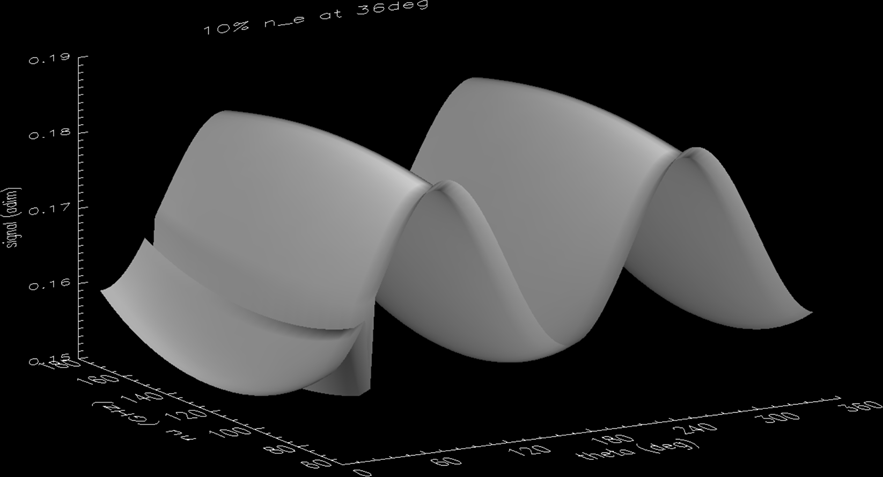
\includegraphics[width=2.5in]{figures/hwp_nonuniform.png}
%\caption{2$f$ signal from a (1,0,0,0) Stokes vector incident on a HWP with a localized non-uniformity: a discontinuous increase of
%10$\%$ of the extraordinary index at theta=36${\circ}$}.}\label{hwpnonuniform}
%\end{figure}

\subsection{Sapphire HWP Degredation Over Time}

\paragraph{Description:} 
% Description of systematic effect, including relevant equations and
% parameterization for TWGs. Note that each variable in each equation should be
% defined. This should include where we expect to get the value of this variable
% from (TWG, literature, etc.)

One concern for the HWP is degredation of the modulator performance over time. A few causes for such degredation are

\begin{enumerate}
	\item AR coating delamination
	\item AR coating degredation, for instance due to UV-induced deterioration
	\item Birefringent substrate material degredation, for instance due to cracking
	\item Birefringent substrate moving around inside the rotor, therefore adjusting its angle with respect to the encoder
	\item HWP becoming dirtied by the environment
\end{enumerate}

POLARBEAR is now in its fourth season using a sapphire modulator \cite{PB1_WHWP}. The PB HWP consists of a sapphire substrate with an AR coating of RT6002 Duroid from Rogers Corporation adhered with melted LDPE. The HWP is located between the primary and secondary mirrors (i.e. at prime focus) and is covered with a thin Mylar sheet for environmental protection. PB has not seen evidence of HWP degredation despite snowstorms, dust, windy weather, etc. The Mylar sheet must be cleaned periodically.

For the POLARBEAR-2a warm HWP (WHWP) \cite{PB2a_WHWP}, we are using a three-stack sapphire HWP with RT3006 Duroid/HDPE dual-layer AR held onto the sapphire using a vacuum-bag technique (i.e. no glue layers). The HWP sits in front of the optics tube window and is protected from the environment by a weather-sealed boom enclosure. The vacuum technique avoids the possibilities of AR delamination and non-uniform glue-layers. To prevent the three sapphire plates from rotating with respect to one another, we epoxy them together at the edges, and to prevent the stack from shifting in the rotor, it is held snugly by a rubber gasket as well as the friction of the vacuum bag. Another concern for HWP degredation is UV eroding the HDPE quality, but we expect this effect to be small given the UV-tight quality of the boom enclosure.

For the POLARBEAR-2b/c cold HWP (CHWP), we are using three-stack sapphire with alumina thermal spray loaded with nitrogen-infused silica microspheres to adjust the dielectric constant. The HWP will sit behind the cryostat window at the 50\,K stage. An additional concern for the CHWP is the danger of AR delamination due to differential thermal contraction during thermal cycles. However, the alumina-powder-based thermal-spray AR has the same expansion coefficient as the sapphire substrate, and there has been no evidence of delamination in testing.
  
\paragraph{Plan to model and/or measure:}
%Plan to model/measure effect
The impact of these effects can be mitigated through regular monitoring and mitigated through the design/repair of the HWP.

For the WHWP, because it is outside the receiver, load curves can be taken by doing in-and-out tests between seasons to look for uniform degredations of the dielectric layers that would cause an increase in emission. Visual inspections can also be used to monitor the HWP. Non-uniform degredations, such as AR delamination, will show up in the HWPSS, or if egregiuos enough, in beam maps. These effects depend on where your HWP is located within the optical system.

In a cryogenic system, the HWPSS and beam maps as a function of time can be used to track HWP degradation.

This effect has an SRF of 2 because the effect is small and can be monitored as well as mitigated with the HWP design.

\paragraph{Uncertainty/Range:}
%This section should include the uncertainty of
%known parameters and/or the expected range of parameters for consideration

The acceptable range of these effects are difficult to quantify, but we should not tolerate AR delamination or shifting of the birefringent substrate in the design process. 

\textbf{How big are these effects when they have shown up on PB? Based on the location of the HWPs in SO, do we expect it to be bigger or smaller? Is it more important at UHF frequencies?}

\paragraph{Parameterization:}

Parameters for the sensitivity and systematics include:

\begin{enumerate}
	\item HWP efficiencyas a function of time $\eta(t)$
	\item HWP emissivity as a function of time $\epsilon(t)$
	\item HWP loading due to scattering as a function of time $P_{HWP, \, scatter}(t)$
	\item HWPSS over time
\end{enumerate}	

\subsection{Metamaterial Degredation Over Time}

\paragraph{Description} 
% Description of systematic effect, including relevant equations and
% parameterization for TWGs. Note that each variable in each equation should be
% defined. This should include where we expect to get the value of this variable
% from (TWG, literature, etc.)

One minor concern for silicon metamaterial HWPs is degredation of the modulator performance over time.  A few causes for such degredation are:

\begin{enumerate}
	\item chipping of the surface structures (AR, or even the birefringent layer)
	\item delamination of glue layer between silicon parts
	\item HWP moving around inside the rotor, therefore adjusting its angle with respect to the encoder
	\item HWP becoming dirtied by the environment
	\item Metallization by UV light
\end{enumerate}

Si metamaterial HWPs are primarily advantageous ove sapphire at ambient temperature, where their smaller thickness due to their refractive indices result in less thermal emission. At cryogenic temperatures, this advantage is lessened because the cooler temperatures result in less overall emission. Thus, we consider only an ambient temperature Si HWP here as in ACTPol/AdvACT. In a three month deployment period, ACT measured no significant chipping or changes in performance.  There may have been a small amount of dust build up in the grooves, but this is not expected to decrease performance.
  
\paragraph{Plan to model and/or measure:}
%Plan to model/measure effect
Most of these effects can be mitigated by careful deisgn and measuremetns of the HWP prior to deployment. They can also be measured and tracked through the HWPSS and HWP performance. Chipping of the substructures occurs primarily in the fabrication process. The pillars are robust to light handling and do not usually break under normal operation. Thus, specifications on the number of chips can be set prior to fabrication as a quality control parameter. Any delamination usually occurs during manufacture, so measurements of the HWP prior to deployment can set a spec on this, and changes in HWP performance can be monitored with the HWPSS. A bossed invar ring glued to the edge of the HWP, keeps the HWP angle fixed to the encoder angle, preventing movement betweeen the HWP and encoder. A zotefoam cover is used on AdvACT to protect the HWP from UV light and dust.

No degredation has been observed on ACT, so the SRF of this effect is 2.


\paragraph{Uncertainty/Range:}
%This section should include the uncertainty of
%known parameters and/or the expected range of parameters for consideration


Preliminary studies have shown that surface chipping of the AR coating does not strongly impact the HWP performance. As many as 1 in 7 pillars chipped shows only a marginal loss in reflection mitigation \cite{SiAR_1}, and the actual pillar yield is significantly better and closer to \textbf{put the typical yield here, note that we can assume we've gotten better in time and use weight later HWPs more}.

%We don't have any estimates for how big effects from delamination, dirt, and UV effect the HWP performance since the HWP from ACT has not yet shown any issues with these.

\paragraph{Parameterization:}
We can parameterize the chipping effect through the effective yield of the AR coating (intact pillars / total pillars). The main effect would be an increase in reflection. Delamination could cause changes in the HWPSS, reflections, scattering, and modulation efficiency problems, so can be parameterized by those.

\subsection{Wobbling}

\paragraph{Description:}
A non uniform HWP mechanical rotation can impact the output signal.
By wobbling we mean a non uniform HWP mechanical rotation. The simplest not uniform rotation is the wobbling, which
we define as a slight change of the HWP rotation axis happening during the HWP rotation itself. In standard HWP rotation, the HWP disc remains parallel to the plane
of its own rotor. If the HWP wobbles, the HWP disc is not anymore parallel.

The reasons can be typically of mechanical origin,
e.g.: excessive play in the HWP mounting support, erroneous HWP mounting in its own support. The wobbling shouldn't be confused with the vibration. By vibration we mean random $a$ movements of the HWP (with $a \ll d$, being $d$ the HWP thickness) in all the directions; with wobbling, instead, we mean random movements of the HWP generated by a precession of the HWP rotation axis. Since different mechanical mismatches are prone to create a wobbling there is not a unique way to model it; therefore, in what follows we have modeled it assuming a simple test model.

For semplicity we can think it changes with time describing
a sinusoidal law. The value of the amplitude and on the phase depends on the HWP rotators and its own imperfections, it cannot be derived
from analytical considerations. A simulation can only provide how a typical wobbling affects the HWP output signal.

Results from the 2$f$ signal generated by a HWP wobbling with the law $5\cos(i)$ (Fig.\,\ref{hwpwobble}), with $i$ the incident angle of the incoming radiation, shows a modest impact on the signal of interest.

\paragraph{Plan to model and/or measure:}
The easiest way to model a HWP wobbling is varying, in a random way, the incident angle of the incoming radiation crossing the HWP.
In case of a macroscopic movement, the effect can be studied just optically observing the behavior of a
reflecting material applied on a rotating HWP. A more quantitative way would require studying the
sideband of 2$f$ or 4$f$ HWP synchronous signal.


\paragraph{Uncertainty/Range:}
Uncertainty could come from a too much naive choice of the sinusoidal law: a simple, and unique, co-sinusoidal law might be not applicable or it might change with time, i.e. it could be described by different co-sinusoidal laws. The uncertainty in the estimate of this effect is ultimately
related to the HWP angle encoder resolution.

\paragraph{Parameterization:}
The most naive way to parameterize the HWP wobbling is assuming an incident angle varying with a co-sinusoidal law.
Since the normal to the HWP and the disc are perpendicular each other, the variation with time of the HWP disc can be translated
into variation of the incident angle. Since is highly unlikely that a wobbling effect will keep the same amplitude across time,
a more realistic parameterization of this effect should consider injecting random angle fluctuations as well.

%SRF: 3(2)*

%\begin{figure}
%\centering
%\includegraphics[width=2.5in]{figures/hwp_wobble.png}
%\caption 2$f$ signal from a (1,0,0,0) Stokes vector incident on a Sapphire HWP wobbling with the incoming radiation varying with the law $5\cos(i)$ with $i$ the incident angle of the incoming radiation.}
%\label{hwpwobble}
%\end{figure}


\subsection{HWP Beam Systematics}


\paragraph{Description:}
Having a HWP skyward of every optical element mitigates a range of beam and polarization systematics. However, when the HWP is further down the optical chain as in the case of a cryogenic HWP, detailed modeling is necessary to determine what systematics it induces and mitigates.

\textbf{Do we have examples of what beam properties get worse?}

\paragraph{Plan to model and/or measure:}
Modeling would require the HWP optical properties and both ray tracing and physical optics for several cases, including non-planar positions and non-uniform AR coatings. The HWP would need to be included in full optics simulations of the optics chain. Commercially available software like CST can model diffraction effects, in a reasonable CPU time, for complicated, large structures, so a model could be developed for the HWPs and serve as input to the larger optical studies.

\textbf{Is there more info on how we can model/measure/calibrate/mitigate this effect? How do we account for mitigation and effects when it is included in the full optics configuration}

Beam maps with and without the HWP can also help determine the HWP's impact on the beams. Measurements, in principle, would be done with a long campaign of beam maps taken at a large set of HWP angle, and/or, in the case of a rapid modulator, very slow beam maps taken with several modulation cycles per beam scanned (differently from sky configuration where the telescope scan is faster). Both unpolarized and polarized beam maps would be necessary.

Optical effects of the HWP must be modeled as there is a large uncertainty in the size of the effect, so the SRF is 5.

\paragraph{Uncertainty/Range:}
\textbf{Do we have any modeled values from SO?}

\paragraph{Parameterization:}
This can be expressed as the beam with and without the HWP from optics simulations.

\subsection{HWP Aliasing}

\paragraph{Description:}
%Description of systematic effect, including relevant equations and
%parameterization for TWGs. Note that each variable in each equation should be
%defined. This should include where we expect to get the value of this variable
%from (TWG, literature, etc.)
HWP aliasing occurs when aliases from the lower harmonics of the $A(\chi)$ signal (0$f$ and 2$f$) leak into the CMB singal band at 4$f$. This is measured as polarization leakage in the 
\textbf{Need more details about this}

\paragraph{Plan to model and/or measure:}
%Plan to model/measure effect. Use SRFs to describe how well we understand/can model the effect. 
%Is there a good null test that we could use to catch this effect?
To model this effect we can use the Mueller matrix to estimate the size of the intensity to $2f$ leakage. (More details, how does this give you the aliasing?)

We can characterize the level of this leakage by observing an unpolarized source. However, this will give the overall polarization leakage of the full instrument and not just the aliasing.

Explain what we can do to mitigate this in the design of the instrument...

This effect directly contaminates the science band, so it is critical that we model it. Thus it has an SRF of 4.

\paragraph{Uncertainty/Range:}
%This section should include the uncertainty of
%known parameters and/or the expected range of parameters for consideration
\textbf{Do we have values of how large this is for the SO SAC? If not, do we have sims that can estimate it? How does it vary with frequency and other parameters? Does it vary with HWP position in the instrument?}

\paragraph{Parameterization:}
%This section should include the parameterization of figures of
%merit and the output to the SWGs.
We can parameterize this effect as an intensity to polarization leakage level in the 4$f$ signal.

\subsection{Encoder Jitter}

\paragraph{Description:} 
% Description of systematic effect, including relevant equations and
% parameterization for TWGs. Note that each variable in each equation should be
% defined. This should include where we expect to get the value of this variable
% from (TWG, literature, etc.)

A source of white noise in the demodulated timestream is encoder jitter, which is governed by how well the HWP angle and bolometer sample are matched in the time-ordered data (TOD). 

During observation, the HWP angle and bolometer samples are read out and timestamped simultaneously by a global trigger, sent to a centralized DAQ device, and paired within a single data packet. In an ideal world, the HWP angle assigned to this timestamp will be correctly obtained and synchronized. However, in reality, the stored HWP angle is not exact but instead exhibits some (presumedly Gaussian white) distribution around the true value. This ``angle jitter'' creates a decorrelation between the rotation-synchronous signal of the HWP and the signal detected by the bolometers. During analysis, this error between the HWP angle the the ``true'' angle experienced by the bolometer (via the HWP-synchronous signal) injects white noise into the demodulated timestream.

Below are a few sources of this timestamp jitter:

\begin{itemize}
 \item \textbf{A noisy encoder waveform} creates a jitter in the interpereted angle of the HWP for each encoder tick. Casues of waveform-induced noise include poor sensor signal-to-noise, a waveform with poorly-defined rising and falling edges (e.g. sloping rather than sharp edges), noisy waveform amplification, and non-rotation-sychronous HWP rotor vibrations.
 \item \textbf{An inadequate encoder sampling rate} prevents precise identification of the encoder ticks. If your encoder readout is sampling the encoder slowly, inerpolation must be used to estimate the HWP angle. Interpolation relies on the smoothness of the HWP rotation and therefore can be noisy if the HWP is vibrating or wobbling.
 \item \textbf{An inadeqaute encoder tick frequency}, in a similar way to an inadequate sampling rate, requires a reliance on interpolation to retrive the HWP angle and therefore can be noisy.
 \end{itemize}
  
\paragraph{Plan to model and/or measure:}
%Plan to model/measure effect

Expected instrumental polarization from optical elements in front of the HWP must be modeled in order to make estimates of the expected power at 4f. This should be modeled using a physical optics simulator with realistic emissivities. Additionally, HWP differential emission and differential reflection should be measured prior to deployment to make estimates of the expected power at 2f. Then, given these expected weights, you can set requirements on the acceptable white noise for your amplifiers, the well-behavedness of your encoder waveform, etc.

This is a small effect, but can become important in cases where the polarization leakage in front of the HWP is large. Thus, it should be modeled and has an SRF of 3.

\paragraph{Uncertainty/Range:}
%This section should include the uncertainty of
%known parameters and/or the expected range of parameters for consideration

This systematic is driven by the size of the 2f and 4f signals of the HWP, which in turn is dependant on the instrumental polarization sky-side of the modulator. For a HWP at prime focus in the Cross-Dragone scenario, (POLARBEAR), the requirement is quite tight--less than 1 arcsecond--where as for a modulator at the stop of a small-aperture telescope (e.g. ABS), the requirement becomes looser.

\textbf{What values would we expect for SO?}

This effect can be averaged down in analysis with interpolation schemes, and is hence improved if the HWP rotational stability is very good over long timescales.

\paragraph{Parameterization:}

The NET induced by this angle jitter is set by the size of the HWP-synchronous signal:
 
 \begin{equation}
 	NET_{jitter} = \frac{\mathrm{d}T}{\mathrm{d}\theta} \sigma_{\theta} 
 \end{equation}

As an example for how to set a requirment on angle jitter, let's say a HWP has a peak-to-peak 4f signal of 0.2 K and that you want to inject $< 10 \%$ white noise into your Q and U channels compared to your per-polarization array sensitivity of 5 $\mu K \sqrt{s}$. You then use the following relations to calculate $\sigma_{\theta}$

\begin{equation}
	\frac{\mathrm{d}T}{\mathrm{d}\theta}  = \frac{0.1 K}{\pi/8 rad}
\end{equation}

where we've assumed that the Q/U signal rises/falls by $A_{p2p}/2$ in $1/16$th of a HWP rotation (i.e. 4f). Then, the angle jitter requirement is given by

\begin{equation}
    	\sigma_{\theta} < \frac{\mathrm{d}\theta}{\mathrm{d}T} NET_{jitter} <  \frac{\pi/8 rad}{0.1 K} (0.5 \mu K \sqrt{s}) < 1.9 \mu rad \sqrt{s}
\end{equation}

The requirement on the white noise should be set by the science working group (SWG). The requirement gets tighter the larger your HWP sychrnous-signal is, hence making large instrumental polarization signals in front of your HWP dangerous.

To convert this angle requirement into a timestamp jitter, which is often more useful for diagnosing aspects of the system like IRIG and RP synchronization, microcontroller performance, etc., you divide the angle jitter by the HWP rotation speed. For the above example, for a 2 Hz HWP, the timestamp jitter requirement is

\begin{equation}
	\sigma_{t} = \sigma_{\theta} / \frac{\mathrm{d}\theta}{\mathrm{d}{t}} = (1.9 \mu rad \sqrt{s}) / (\frac{4 \pi}{s}) = 0.15 \mu s \sqrt{s}
\end{equation}

The requirement on the HWP timestamp accuracy becomes tighter as the HWP rotation frequency increases.

%\subsection{Time Variation of HWP Signal}
\label{IP downstream of HWP}
\paragraph{Description:}
Description of systematic effect, including relevant equations and
parameterization for TWGs. Note that each variable in each equation should be
defined. This should include where we expect to get the value of this variable
from (TWG, literature, etc.)

\paragraph{Plan to model and/or measure:}
Plan to model/measure effect. Use SRFs to describe how well we understand/can model the effect. Is there a good null test that we could use to catch this effect?

\paragraph{Uncertainty/Range:}
This section should include the uncertainty of
known parameters and/or the expected range of parameters for consideration

\paragraph{Parameterization:}
This section should include the parameterization of figures of
merit and the output to the SWGs.


\section{Time Constants}
The time constant of each detector is a key property that describes the stability and time response of the detector. If the time constant is too large, it must be accounted for in the demodulation of the signal from the HWP polarization modulation, in setting the scanning frequency of the telescope, in measuring the telescope beams and pointing, and in determining the polarization angles of the detectors (if using a HWP). The optical time constant $\tau_{opt}$ is often expressed in terms of the 3dB frequency $f_{3 dB}$, which is given by $f_{3dB}=1/(2\pi \tau_{opt})$. There are several ways to measure the detector time constants.

\paragraph{Planet Scan Method} The time constants of the detectors can be probed by scanning quickly over bright objects such as planets, but our ability to probe such features might be limited by the maximum scan speed of the telescope mount and the low signal to noise on an individual planet scan.

\paragraph{Bias Step Method} The bias step method characterizes the electrical time constant of a detector $\tau_{el}$ by inputing a low amplitude square wave through the bias line and fitting the exponential response. The current $I$ as a function of time $t$ goes as
\begin{equation}
I(t) \propto e^{\frac{\pm t}{\tau_{el}}},
\end{equation}
where the exponential is positive as the voltage is increased and negative as the voltage is decreased. The bias step method is quick and easy to perform before measurements, but $\tau_{el}$ must be properly correlated to optical time constant measurements to determine the optical time constant $\tau_{opt}$.

\paragraph{Amplitude Method} With the amplitude method, the time constants are determined by modulating a source with a chopper or stimulator at various frequencies and measuring the amplitude of the detector responses. If a the system includes a HWP, the chopper method required it to be stationary during the measurement. The response in power $P$ of the detectors is given by
\begin{equation}\label{eqn:tc_amp}
P(f) \propto \frac{1}{1+\Big(\frac{f}{f_{3dB}}\Big)^2},
\end{equation}
where $f_{3dB}$ is the optical 3dB frequency and $f$ is the modulation frequency of the source. Figure~\ref{fig:tc_chopper} shows the power versus frequency measurements from two measurements on ABS with their fits~\cite{Simon_Thesis_2016}.

The optical time constant of a detector increases with increasing loading, and with this method, the added loading from the atmosphere near the horizon behind the source can be large enough to drastically slow the detector time constants and, in some cases, fully saturate the detectors, making them non-responsive. Thus, the time constants measured with this method may not be representative of the time constants under typical loading conditions. For example, in ABS, this method gave $f_{3dB} \sim 30$~Hz versus the actual average across the whole season of 109~Hz. Additionally, the measured amplitudes can be highly sensitive to changes in loading correlated to the weather. Without the use of the HWP, the atmosphere can cause fluctuations in the signals on order of a pW. The power versus frequency plot in the left panel of Figure~\ref{fig:tc_chopper} shows that the fluctuations can be larger than the effect from the time constants.

\begin{figure}[h!]
\centering
\includegraphics[width=\textwidth]{figures/ampl_pvfreq.pdf}
\caption{The power versus frequency relations are shown above in green with their fits in black for two time constant measurements on ABS. The large atmospheric fluctuations in the first four frequencies of the first measurement and in the last frequency of the second measurement cause the power to fluctuate more than the effect from the time constant, which can be problematic.}
\label{fig:tc_chopper}
\end{figure}

\paragraph{Phase Method} When an experiment has a HWP, the optical time constants can be characterized using the phase delay of the $4f_{m}$ signal~\cite{Simon_LTD2013}. Because it uses the phase, this technique is less susceptible to atmospheric fluctuations over the course of the measurement than the amplitude method. For each phase method measurement, data are taken while slowly varying the rotation speed of the HWP with a sparse polarizing wire grid positioned above the HWP. The wire grid is used to input a small ($\sim0.1$ pW) polarized signal. This signal adds minimal loading, so the time constants are closer to those during nominal observation. The phase $\phi$ found from demodulating the signal with respect to the polarization modulation frequency $4f_{m}$ is the difference between the physical polarization angle of the grid and the measured polarization angle, which includes the apparent angle rotation due to the time delay of the detector response. It can be modeled as the phase of a one-pole filter: 
\begin{equation}\label{eqn:phi_shift}
\phi=\arctan{\left(\frac{4f_{m}}{f_{3dB}}\right)} + C,
\end{equation}
where $f_{3dB}$ is the optical 3dB frequency of the detector. Because $(4f_{m})^2$ is expected to be much less than $f_{3dB}^2$, the phase can be linearly approximated as 
\begin{equation}
\phi  \approx \phi_0 + \frac{f_{3dB}\,4f_{m}}{f_{3dB}^2+(4f_{m})^2}\approx  \phi_0 + \frac{4f_{m}}{f_{3dB}},
\end{equation}
where $\phi_0$ is a constant offset related to the intrinsic polarization angle of the detector~\cite{Simon_LTD2013}. 

\subsection{Polarization Angle Rotation with Time Constant}

\paragraph{Description:}
In an experiment that employs a continuously-rotating HWP, fluctuations in the time constants of the detectors between observations can cause apparent shifts in the polarization angles of the detectors. This effect is of particular importance when calibrating the polarization angles of the detectors. The magnitude of the angle shift from the detector time constant is half the offset in phase, which is given by Equation~\ref{eqn:phi_shift}. In the case where $f_{3dB}$ is constant throughout all CMB observations, the angle shift can be neglected, so the primary concern is the secondary effect of fluctuations in the angle shift between CMB measurements~\cite{Simon_Thesis_2016}.

The direction of the angle shift is dependent on the coordinate system of the polarization angle definition and the rotation direction of the HWP. In all cases, the shift in phase is in the direction of the HWP rotation. The Healpix convention defines the coordinate system such that the vertical polarization angle is $\psi=0^{\circ}$ and the horizontal polarization angle is $\psi=90^{\circ}$. The sign in this treatment assumes that the HWP rotates in the positive direction in this coordinate system. Using a wire grid to measure the polarization angle as described in~\cite{Tajima_2012}, the measured angle $\psi_{meas}$ is defined as
\begin{equation}
\psi_{meas} \equiv 1/2 \arctan{(U/Q)}=1/2\mathrm{arg(demod)}=\psi_{WG}-\psi_{det},
\end{equation}
where $Q$ and $U$ are the Stokes parameters, arg(demod) is the phase argument of the demodulated timestream, $\psi_{WG}$ is the angle of the polarized signal from the wire grid, and $\psi_{det}$ is the polarization angle that the detector is sensitive to when the HWP encoder value is zero. The phase $\phi$ is equal to arg(demod), which gives
\begin{equation}
\psi_{det}=-\frac{1}{2}\phi + \psi_{WG}.
\end{equation}
Expanding the phase into $\phi=\phi_{0}+2\Delta \psi$ and using Equation~\ref{eqn:phi_shift}, we can then write the detector angle as
\begin{equation}
\psi_{det}=-1/2\phi_{0}-\Delta \psi+ \psi_{WG}=\psi_{det,0}-\Delta \psi + \psi_{WG}=\psi_{det,0}-1/2\arctan{\left(\frac{4f_{m}}{f_{3dB}}\right)} + \psi_{WG}\,\, ,
\end{equation}
where $\psi_{det,0}$ is the intrinsic polarization angle of the detector~\cite{Simon_Thesis_2016}.

\paragraph{Plan to model and/or measure:}

In this case, the angle shift is in the negative direction, so $\Delta \psi$ must be added to the polarization angles of the detectors for all observations and polarization angle measurements to correct for this effect. For each observation, $\Delta \psi$ can be determined using the HWP rotation frequency $f_{m}$ from the HWP encoder and the optical $f_{3dB}$ for the detector timestream. When taking IV curves for wire grid polarization angle measurements, the wire grid should be in place to get a more accurate time constant estimation. The dependence of this effect on $f_{3dB}$ means that we must have an understanding or measurement of the time constants for each CMB observation. To achieve this, several optical time constant measurements can be used to determine the conversion factor between the electrical and optical time constants. Then the IV curves before each observation can be used to determine the electrical time constants, which can be converted to optical time constants with the conversion factor as was done in ABS~\cite{Simon_Thesis_2016}. A null test that splits the detectors based on their median $f_{3dB}$ values could catch this systematic. One could also run the analysis with and without this effect accounted for to determine the level of systematics as was done in ABS.

This can be further mitigated by having fast time constants, which is not as constrained in DfMux and $\mu$Mux systems as it is in TDM systems.

This effect directly impacts the polarization angle rotation and requires a good understanding of the detector time constants, making its SRF a 4. This effect is not present with no HWP.

\paragraph{Uncertainty/Range:}
The size of this effect depends on the modulation frequency of the HWP $f_{m}$ and the optical $f_{3dB}$ of the detectors. Faster time constants and slower $f_{m}$ have a smaller effect. To first order, these effects are on the order of degrees, but if the $f_{3dB}$ is constant, this effect can be easily corrected. However, the secondary effect of the polarization angle fluctuating with fluctuating $f_{3dB}$ is the primary concern. For a low 3dB frequency of 30~Hz (most experiments have an average $f_{3dB}>100$~Hz) and a modulation frequency of 10.2~Hz, a 10\% shift to a lower $f_{3dB}$ results in a $0.96^{\circ}$ shift in polarization angle. ABS has shown that this can be successfully corrected to a few percent, but this requires a good understanding of the optical $f_{3dB}$, which is the main source of uncertainty.

\paragraph{Parameterization:}
This effect is parameterized with $\Delta \psi=-1/2\arctan{\left(\frac{4f_{m}}{f_{3dB}}\right)}$. Note that the sign of the effect depends on the coordinate system and the direction of the HWP rotation.

\subsection{Time Constant Effect on Beam and Pointing}

\paragraph{Description:}
The time constants can both shift the detector pointing and smear the beam, resulting in an increase in the measured beam width. To estimate these effects, the beam can be approximated as a Gaussian with a full width at half maximum of $FWHM$. The experiment is assumed to scan at a rate of $f_{scan}$ at an elevation $\theta_{el}$. The scanning speed on the sky $f_{sky}$ is then given by $f_{sky}=f_{scan}\cos{(\theta_{el})}$. The time domain Gaussian beam $\beta (t)$ is then defined as
\begin{equation}
\beta (t)=e^{\frac{-t^2}{2\sigma^2}},
\end{equation}
where $t$ is time and 
\begin{equation}
\sigma=\frac{FWHM}{2f_{sky}\sqrt{2\ln2}}.
\end{equation}
Fourier transforming into frequency space, the beam is given by 
\begin{equation}
\beta (f)=e^{-2 \pi^2 f^2 \sigma^2}.
\end{equation}
The time constants of the detectors act as a low pass filter, so the beam is convolved with a low pass filter given by
\begin{equation}\label{eqn:low_pass}
h(f)=\frac{1-if/f_{3dB}}{1+f^2/f_{3dB}^2}
\end{equation}
and then Fourier transformed back into the time domain to determine the impact on the pointing and beam widths. This treatment assumes that the low pass filter in Equation~\ref{eqn:low_pass} is a good approximation in the range of 3dB frequencies expected for the detectors. Figure~\ref{fig:tc_shift} shows the effect from varying 3dB frequencies on the beam for ABS, which had a $FWHM \approx 30$~arcmin and $f_{sky}\approx 0.5$~deg/s. These calculations give the shift and change in beam width for scanning in one direction, but the telescope scans in both directions. If there are an equal number of scans in each direction, the pointing offset averages out, but an odd number of scans could give a pointing offset. Thus, the above calculation gives the maximum pointing offset $\Delta p_{max}$. The effect of scanning both ways further broadens the beam because the average measured beam is the sum of two offset beams as illustrated in Figure~\ref{fig:tc_beam_shift}. To account for this, the two beams from scanning in either direction are approximated as two Gaussian beams and a Gaussian is fit to their sum. From this, $\Delta FWHM$ can be calculated~\cite{Simon_Thesis_2016}. 

\begin{figure}[h!]
\centering
\includegraphics[width=0.90\textwidth]{figures/time_constant_shift.pdf}
\caption{The shift in the pointing and the beam width for an ABS scan in one direction as a result of several time constants is shown above~\cite{Simon_Thesis_2016}. Note that 3dB frequencies above 5~Hz have an extremely small effect. The power is in arbitrary units.}
\label{fig:tc_shift}
\end{figure}


\begin{figure}[h!]
\centering
\includegraphics[width=0.80\textwidth]{figures/half_hertz_shift.pdf}
\caption{The shift in the beam width from the time constant when scanning in both directions is estimated with the sum of two Gaussians shifted in pointing and beam width in opposite directions. This can be approximated and fit as a Gaussian. The shift for an extremely slow detector with an $f_{3dB}=0.5$~Hz is shown above for ABS to illustrate this effect~\cite{Simon_Thesis_2016}. The power is in arbitrary units.}
\label{fig:tc_beam_shift}
\end{figure}

\paragraph{Plan to model and/or measure:}

This effect is usually negligible, but it can be approximated as described above quickly and easily given a $f_{3dB}$ value, beam width, scanning frequency, and elevation. If the beam is well known, planet scans can be used to determine $\Delta FWHM$ and $\Delta p_{max}$ (though these measurements usually have low signal to noise). Designing the experiment to have a fast time constant also minimized this effect. A null test split on fast versus slow time constants could help determine if this effect is contaminating the signal, but this null test split is redundant with other time-constant related systematics like the polarization angle rotation. 

Given that we can model this effect well and that it is expected to be small, its SRF value is 3.

\paragraph{Uncertainty/Range:}
With the typical $f_{3dB}$ values for CMB experiments, this effect is often negligible, but it is good to check. When modeling this effect, the main uncertainties come from the time constants of the detectors and assuming a purely Gaussian beam. Typically, one can just use the lowest $f_{3dB}$ value expected/measured to put an upper bound on this effect. If the upper bound is negligible, then this effect will be negligible at all higher $f_{3dB}$ values as well. Table~\ref{table:tc_shift} summarizes the impact of the time constants on the ABS beam, which is a similar size to the SO small aperture camera, for various 3dB frequencies.

\begin{table}[h!] 
\begin{center}
  \caption {\textbf{Impact of 3dB Frequency on Beam and Pointing}}\label{table:tc_shift}
\begin{tabular}{|l|l|l|}
  \hline                        
  \textbf{3dB Frequency (Hz)} &  \textbf{Pointing Shift (arcmin)} &  \textbf{$\Delta$ FWHM (arcmin)} \\
  \hline
  0.5 & 7.353 & 10.5 \\
  \hline
  1.0 & 4.313 & 3.7 \\
  \hline
  5.0 & 0.950 & 0.17 \\
 \hline  
  10.0 & 0.477 & 0.043 \\
 \hline  
  20.0 & 0.239 & 0.011 \\
 \hline  
  30.0 & 0.159 & 0.0047 \\
 \hline  
  40.0 & 0.119 & 0.0026 \\
 \hline  
  50.0 & 0.096 & 0.0016 \\
 \hline  
  100.0 & 0.048 & 0.00052 \\
 \hline  
\end{tabular}\\
The pointing shift and beam width changes from different 3dB frequencies are shown above. The typical 3dB frequency of the ABS detectors is $\sim$109~Hz, and the lowest $f_{3dB}$ that passes the data selection criteria is greater than 30~Hz~\cite{Simon_Thesis_2016}.
\end{center}
\end{table}

\paragraph{Parameterization:}
This effect can be parameterized with $\Delta FWHM$ and $\Delta p_{max}$ for a given $f_{3dB}$ value.

\subsection{Time Constant Calibration Error (Kevin)}

\paragraph{Description:}
%Description of systematic effect, including relevant equations and parameterization for TWGs. Note that each variable in each equation should be defined. This should include where we expect to get the value of this variable from (TWG, literature, etc.)

Depending on the technique used to calibrate the thermal-response of the timestream, there might be several science scans taken in between calibration measurements. In between calibration measurements, the thermal calibration of each detector and its time constant can significantly drift from its initial value. Here sensitivity is defined at dP/dI and gain is defined as dT/dI or (dT/dP)*(dP/dI). Measurements of planets and known temperature sources like a stimulator give defined gain while studies of loopgain variation give sensitivity information. With a fixed voltage bias on a TES in the strong electrothermal feedback regime the total power on the detector is fixed so the electric bias power will change to compensate for changes in optical power: $\Delta P_{opt}=-\Delta P_{bias}$. The TES Loopgain, $\mathcal{L}$, is linearly proportional to $P_{bias}$ so as the detector sees changes in atmospheric and instrumental loading $\mathcal{L}$ varies. Although we are looking at gain stability here, the bolometers thermal time constant is also sped up under electrothermal feedback by the relationship (\ref{eq_timevar_1}) as given by Irwin \& Hilton \cite{Irwin_Hilton}. So variations in loopgain will effect both sensitivity and the time constant over an observation.
\begin{equation}
\label{eq_timevar_1}
\tau_{ETF}=\tau_0\frac{1+\beta_I+R_L/R_0}{1+\beta_I+R_L/R_0+(1-R_L/R_0)\mathcal{L}}
\end{equation}
$\tau_0$ is the intrinsic thermal time constant $G_0/C$. The power to current sensitivity (also called ``responsivity`` in ACT), $s_I(\omega)$ is also dependent on $\mathcal{L}$ and is given by (\ref{eq_timevar_1})
\begin{equation}
\label{eq_timevar_2}
s_I(\omega)=\frac{-1}{I_0R_0}\left(\frac{L}{\tau_{elec}R_0\mathcal{L}}+(1-\frac{R_L}{R_0})+i\omega\frac{L\tau_0}{R_0\mathcal{L}}(\frac{1}{\tau_{ETF}}+\frac{1}{\tau_{elec}})-\frac{\omega^2\tau_0L}{\mathcal{L}R_0}\right)^{-1}
\end{equation}
Where $R_0$ is the resistance on the transition where the bolometer is initially biased to, $R_L$ is the shunt resistor in parallel with the TES, $\tau_{elec}$ is the electrical time constant, $I_0$ is the required current to initially set the TES at $R_0$, and $L$ is the inductance in the TES bias/readout circuit, and $\beta_I$ is the logarithmic derivative of TES resistance with current. The limits that we typically take for our experiments is $R_L/R_0 \ll 1$, $\beta_I \ll 1$, $\tau{elec} \ll \tau_{ETF}$, and $\tau{elec} \ll \tau_0$. Taking this limit from (\ref{eq_timevar_1}), $\tau_{ETF} \simeq \frac{\tau_0}{\mathcal{L}+1}$, and $\tau_{elec} = \frac{L}{R_L+R_0}$. Equation (\ref{eq_timevar_2}) also reduces  significantly to (\ref{eq_timevar_3})
\begin{equation}
\label{eq_timevar_3}
s_I(\omega) \simeq \frac{-1}{V_{biax}}\left(\frac{\mathcal{L}}{\mathcal{L}+1}\right)\left(\frac{1}{1-i\omega\tau_{ETF}}\right)\left(\frac{1}{i\omega\tau_{elec}-1}\right)
\end{equation}
Since $\tau{elec} \ll \tau_0$, we often just consider a narrow frequency band around the carrier tone and ignore the second pole from the electric transfer function, so equation (\ref{eq_timevar_3}) can be written as (\ref{eq_timevar_4}).
\begin{equation}
\label{eq_timevar_4}
s_I(\omega) \simeq \frac{-1}{V_{biax}}\left(\frac{\mathcal{L}}{\mathcal{L}+1}\right)\left(\frac{1}{1-i\omega\tau_{ETF}}\right)
\end{equation}
To account for mean optical power drifts in time periods between rebiasing of the bolometer we must either come up with a model for how mean optical power is changing on these time scales or find a way to actively measure it so that we can calibrate out effects on responsivity and time-constants.

\paragraph{Plan to model and/or measure:}
%Plan to model/measure effect. Use SRFs to describe how well we understand/can model the effect. Is there a good null test that we could use to catch this effect?
A possible procedure to correct for time variation over the duration of a science scan is to interpolate our gains between measurements of the thermal calibration source taken at the beginning and end of the observation periods. To understand the impact of potential errors in this interpolation, we can construct a set of gains based only on the initial (or final) calibration measurement thus use no interpolation. Say now that a simulated map with no $B$-modes is ``observed,'' producing timestreams using the non-interpolated gain model, and then reconstructed using the interpolated analysis gain model.  The level of resulting \clbb\ (null to start with) quantifies the difference in these gain models in power spectrum space, and thus puts an upper limit on the impact of the drifts. Bias steps before/after observations, a stimulator, the HWP harmonics, and the atmosphere can all be used for time constant/gain corrections in time.

\textbf{SRF}

\paragraph{Uncertainty/Range:}
This section should include the uncertainty of
known parameters and/or the expected range of parameters for consideration

\paragraph{Parameterization:}
This section should include the parameterization of figures of
merit and the output to the SWGs.


\section{Crosstalk}
\subsection{Crosstalk for DfMux}

\paragraph{Description:}
The frequency multiplexing readout has crosstalk due to the finite width of the LC resonators.
Crosstalk from one bolometer to another due to coupling in the multiplexed readout will lead to polarization and temperature leakage from a point outside the main beam, creating a localized, polarized near side lobe. Crosstalk is strongest in bolometer channels that share a SQUID in the frequency-domain multiplexed readout, and are closest together in bias frequency. Below we look to describe the DfMux system and its crosstalk in slightly more detail but detailed accounts can be found in \cite{Barron_Thesis} and \cite{DfMux_Dobbs2012}.

In the DfMux system we put each TES in series with an inductor and capacitor and tile these RLC ($R=R_{TES}$ + stray series resistance) units together in parrallel with one bias resistor in parrallel to set the voltage bias across the "comb" of RLC's. This results in each TES having a characteristic AC bias frequency set by its respective LC (L fixed, C varied) series pair between 1 and 6 MHz. A set of LC (currently up to 68x for SPT-3G\cite{SPT3G_DfMux_Overview}) is readout by a series array SQUID, which has a per channel feedback to linearize, minimize noise, and maximize the dynamic range of the SQUID called Digital Active Nulling (DAN)\cite{DfMux_LC_Production}. The DfMux warm readout sets a bias and demodulation channel at each of the comb frequencies and monitors the amplitude at each demodulation channel. As the TES experiences resistance changes with changes in incoming power its amplitude modulates its respective lorentzian peak height, and this change in current amplitude is the signal read out on the demodulation channel. 

There are three primary modes of crosstalk present in the DfMux system: bias carrier leakage, non-zero wiring impedance (cold wiring), and inductive/capacitive wiring crosstalk (in warm cables or from physically close conductors in the system). These three types of crosstalk are discussed below with some discussion of how to minimize them. \cite{DAN_Crosstalk_Memo} We then discuss briefly what sorts of systematic effects on our measurements these forms of crosstalk will have. 

\setcounter{equation}{0}
\paragraph{Bias Carrier Leakage}
This variety of crosstalk involves the lorentzian tail of the LRC resonance in frequency space overlapping with neighboring peaks such that some amount of current meant to bias TES $n$ at frequency $\omega_n$ is biasing TES $n\pm1$ at frequency $\omega_{n\pm1}$. The current seen by neighboring channels from channel n, $I^{\omega_n}_{n\pm1}$, is given by
\begin{equation}
I^{\omega_n}_{n\pm1} = \frac{V^{\omega_n}_{bias}}{R_{TES}+i\omega_nL+(i\omega_nC_{n\pm1})^-1} \simeq \frac{V^{\omega_n}_{bias}}{2i\Delta\omega L}\left(1+\frac{iR_{TES}}{2\Delta\omega L}\right).
\end{equation}
By taking the ratio of the current modulation on neighboring channels compared to on a given channel as shown below, we can get the approximate level of crosstalk $|R^2_{TES}/(2\Delta \omega L)^2|$. This comes out to $\sim0.25\%$ for \pb.
\begin{equation}
\frac{\Delta I^{\omega_n}_{n\pm1}}{\Delta R_{TES}} \simeq \frac{V^{\omega_n}_{bias}}{2\Delta\omega L}
\end{equation}
\begin{equation}
\frac{\Delta I^{\omega_n}_{n}}{\Delta R_{TES}} \simeq \frac{-V^{\omega_n}_{bias}}{R^2_{TES}}
\end{equation}

\paragraph{Non-zero Wiring Impedance}
Non-zero impedance in the cold wiring can come from stray impedances in between the bias resistor due to leads, stray series resistance, and the SQUID's input coil. In our system the stray impedance, $Z_{stray}$, is dominated by stray inductances, $L_{stray}$. This creates a modification of the combs voltage bias proportional to the current through a given channel which in turn modulates the current in neighboring channels. With a constant $V_{bias}$ the total change in voltage across the comb is given by
\begin{equation}
dV_{tot}=-dV_{stray}\simeq dI^{\omega_n}_{n}i\omega_nL_{stray}.
\end{equation}
This voltage induces a current in the nearest neighbor channels as defined by
\begin{equation}
dI^{\omega_n}_{n\pm1}=\frac{dV_{tot}}{Z^{LCR}_{n\pm1}}\simeq \frac{-dI^{\omega_n}_{n}\omega_nL_{stray}}{2\Delta \omega L}.
\end{equation}
The ratio of power changes in a channel compared to its neighbors, given below, quantifies this level of crosstalk. For POLARBEAR this is $\sim0.3\%$.
\begin{equation}
\frac{dP^{\omega_n}_{n\pm1}}{dP^{\omega_n}_{n}}\simeq \frac{-dI^{\omega_n}_{n\pm1}\omega_nL_{stray}}{dI^{\omega_n}_{n}\Delta\omega L}
\end{equation}
\paragraph{Other Sources of Crosstalk}
\begin{itemize}

\item Inductors are fabricated on the same board and there is some finite mutual inductance between physically close inductors. This crosstalk is minimized by keeping the mutual inductance coupling coefficient low ($\sim$ 0.01 for POLARBEAR) and physically separating inductors that are close in frequency space. 
\item Crosstalk in the warm cabling between the SQUID and the warm electronics where demodulation and DAN feedback computation occurs can create imperfect nulling which produces excess loading and noise on the SQUIDs. Shielded cables were developed that kept crosstalk between twisted pairs at 60dB between 0.1-10 MHz for POLARBEAR~\cite{DfMux_Warm_Crosstalk_Memo}.
\item Crosstalk has been seen between LC boards. Specifically ones that share a PCB board. There have been some ongoing studies about possible inductive coupling between LC boards. %John Groh, \& Darcy Barron on POLARBEAR and many SPT-3G members have been studying this.
\end{itemize}

\paragraph{Plan to model and/or measure:}

Crosstalk appears as a beam effect and is best understood in map space as a convolution with some crosstalk kernel and in timestream space as a mixing matrix applied to the timestreams of all the detectors.
If the pixel-pixel separation scale is substantially larger than the beam width (i.e. the beams do not overlap), this just looks like a multi-modality of the beam of the receiving detector.
Since the secondary mode(s) of the beam are spatially colocated with the beams of another detector, and share an identical temperature and polarization pattern, the crosstalk mixing matrix can be easily measured from beam maps on point sources.
Most of the effects outlined above are not time-variable, so the values hold permanently and do not need frequent calibration.
This is especially true if one crosstalk mechanism dominates, in which case an appropriate choice of units will remove dependence on bias point.
The efficacy of this technique depends on the available point-source signal-to-noise and is thus easier on large-aperture instruments than small-aperture ones.

\pb\ assumed a constant level of crosstalk between neighbour bolometers, which is not realistic and leads to underestimates of crosstalk-induced bias.
We may want to have a spatial distribution across the focal plane for more realism, with substantial scatter; the effects of crosstalk on calibration measurements must also be taken into account.

There are a few primary pernicious effects of crosstalk on analysis:
\begin{enumerate}
\item{Because the dominant mechanisms have uniform signs, it suppresses the apparent temperature response of the detector. This leads to overestimated polarization efficiencies and a multiplicative bias in polarization power spectra.}
\item{It causes a beam distortion, changing the high-$\ell$ temperature spectra.}
\item{It mixes polarizations together with some spatial pattern, leading to apparent polarized sidelobes. This causes T$\rightarrow$P leakage as well as E$\rightarrow$B leakage.}
\item{It can mix frequencies together on multichroic focal planes, which thwarts foreground cleaning.}
\end{enumerate}

By measuring the crosstalk matrix as described above, most of these effects can be eliminated.
The matrix is, in general, time-invariant and so can simply be inverted and applied to the detector TOD to remove crosstalk entirely.
This approach is being used for all current SPTpol analyses and is extremely effective (2 or more orders of magnitude suppression) if applied at the earliest possible moment in data processing.

The beam map approach is limited, however, in that it can only identify the correct pixel for the origin of crosstalk and not, in general, the correct source polarization or band.

In the polarization case, this does not matter that much in the end.
Intra-pixel polarization crosstalk just appears as reduced polarization efficiency and will be fully calibrated, if not removed, by whatever technique is applied to measure polarization efficiency.
Inter-pixel cross-polarization crosstalk is trickier, but is mitigated by several factors.
First, for the dominant concern of T$\rightarrow$P leakage, the apparent polarization angle of the \emph{receiving} detector matters much more than the \emph{sending} detector, since the source is by definition unpolarized and so the signal to be removed will be the same no matter the identity of the sending detector.
In the event that we deploy a rapid polarization modulator, it also immediately eliminates this source of T$\rightarrow$P, just as it does for all beam effects.
Second, for E$\rightarrow$B leakage, there is little issue so long as the leakage is random.
Unlike the bias in temperature caused by the preferred sign of the off-diagonal crosstalk matrix elements, there is in general no preferred polarization rotation unless unfortunate choices are made in frequency scheduling.
Such choices should be avoided in the design phase.

The most dangerous of these is inter-band cross-talk, as that is the hardest to calibrate out.
Figuring out the source band requires a suite of point sources with different spectra and is subject to large uncertainties; measuring it in detail requires detailed wideband FTS scans of every detector, which are substantially more time and labor intensive than planet observations.
This is best avoided by scheduling the different bands far apart in frequency or, ideally, on different SQUIDs altogether. \textbf{Are there other smart choices we cna make to minimize this?}

The crosstalk needs to be modeled and measured. It can be minimized by making smart design decisions and is thus a design driver, making its SRF a 5.

\paragraph{Uncertainty/Range:}
As a first start, we define two cases.
Each bolometer draws a leakage coefficient from a normal distribution with G1 = ($\mu=-0.3\%,\, \sigma=0.1\%$) or G2 = ($\mu=-3\%,\, \sigma=1\%$).
\textbf{Are these realistic values for SO? How do LAT and SAC differ?}

\textbf{summarize some of the main results on crosstalk from the sims}

\paragraph{Parameterization:}
The instrument systematic pipeline developed for SO aims at more realism than what was done originally for \pb. 
Here is the setup put in place to study the impact of having crosstalk (in a generic way, i.e. leakage from one detector to others):
\begin{enumerate}
\item{We assume a fixed total number of detectors for the focal plane.}
\item{Using this total number of detectors, we assume different focal plane configurations (see Table 1 \textbf{This table doesn't exist}) according to the MUX factor (number of bolometers/SQUID).}
\item{We generate corresponding TODs.}
\item{Each bolometer draws a leakage coefficient from a range of values defined above (G1 or G2).}
\item{This distribution is the same then for all CESes (i.e. leakage is constant in time). Note that time-varying crosstalk is also available in the pipeline, but not used here. \textbf{Is the time variation in crosstalk a secondary effect?}}
\item{According to the Friend Factor (FF), which defines the nearest bolometer indices B communicating with bolometer b in its SQUID: 
\begin{equation}
B = \{ b2\, |\, 0 < |b-b2| \leq FF \},
\end{equation} 
we propagate the crosstalk effect in all the TODs. We chose FF to be either 1, 3, or the total number of bolometers in the SQUID.}
\item{We estimate the sky maps from contaminated TODs, and compute angular power-spectra to determine the polarization leakage.}
\end{enumerate}
\url{http://simonsobservatory.wikidot.com/instrument-systematic-systmodule}.
\textbf{summarize some of the main results}

\textbf{references are commented out and should be added to the dictionary references}
%\subsubsection{References}
%\begin{itemize}
%\item Barron, D., "Precision measurements of cosmic microwave background polarization
%to study cosmic inflation and large scale structure," UCSD Dissertation, (2015).
%\item Dobbs M., "DAN Cable Crosstalk," McGill Memo, (2012). - Not published ask to share.
%\item Montgomery, J., "Cable and Mezzanine Crosstalk," McGill Memo, (2013). - Not published ask to share.
%\item Bender, A. N., "Integrated Performance of a Frequency Domain Multiplexing
%Readout in the SPT-3G Receiver," SPIE, (2016).
%\item Rotermund, K., "Planar Lithographed Superconducting LC Resonators for Frequency-Domain Multiplexed Readout Systems," Journal of Low Temp Phys, (2016).
%\end{itemize} 

\subsection{Crosstalk for $\mu$Mux (Brad, KTC editing)}

\paragraph{Description:}
In the $\mu$mux readout system, we expect cross-talk from the overlap of the Lorentzian resonator profiles in the frequency domain. In the particular case of flux ramp demodulation, this effect should scale as $\frac{1}{2 \pi \times 16 n^2}$, where $n$ is the resonator spacing in units of the resonator bandwidth [Ben Mates thesis] \cite{Mates_thesis}. Reported measurements in [Dober et al. 2017] indicate that the expected 0.025\% for the $n = 20$ system under test is approximately correct for a majority of channels in the system, while 0.3\% forms an upper bound for all channels studied.

\paragraph{Plan to model and/or measure:}
SRF = 3, since there are methods to investigate the effects of crosstalk across entire arrays in various contexts. In the lab, the effect can be measured by introducing small signals into detector channels and looking for the appearance of those signals in other channels. In the field, we can study microwave signal crosstalk using detecor covariances during CMB scans and ``ghost images'' of bright point sources in channels not meant to point at the source itself.

\paragraph{Uncertainty/Range:}
Measurements in [Dober et al. 2017] place a rough upper bound of 0.3\%. Simulations of DfMUX crosstalk show that this level of signal leakage should not affect science results, but that care is needed to determine what the relationship of nearest-neighbor channels is with regard to frequency band, polarization, etc.

\paragraph{Parameterization:}
TBA

\subsection{Time-Domain Multiplexing Crosstalk}

\paragraph{Description:}
We define electrical cross-talk the systematic by which an electrical pick-up generates a signal in a detector that is not supposed to receive any signal.
In a DTM readout schema detectors are read out grouped by bias lines. In presence of electrical cross-talk an electrical signal, injected in a given bias line, appears in other(s) detector(s) fed by completely different bias line(s). 




Description of systematic effect, including relevant equations and
parameterization for TWGs. Note that each variable in each equation should be
defined. This should include where we expect to get the value of this variable
from (TWG, literature, etc.)

\paragraph{Plan to model and/or measure:}
The electrical cross-talk can be probed with the bias step technique, injecting a bias step signal in a single given bias line and looking at the detectors correlation matrix. The method is pretty robust, it takes few seconds per bias lines and it can be performed both in laboratory and in the field configuration. The correlation matrix is expected to by symmetric. In building the correlation matrix the elements on the diagonal, the detectors belonging to the same bias line under study and the detectors listed on the deadlist should be removed (the first and the second ones because they are expected to have correlation equal/close to 1).
However, the correlation matrix built with just the Pearson coefficient does not discriminate between detectors with high amplitude signal and small correlation and detectors with low amplitude signal and high correlation: both will have the same correlation level.
In order to break this degeneracy one possibility is to normalize the Pearson coefficient to the maximum amplitude of the detector signals. 

If $S_{i}(t)$ and $S_{j}(t)$ are the detectors timestreams for the $i$-th and $j$-th detectors, respectively and $< ...>$ the time average of the detector timestream, the normalized Pearson coefficient can be estimated as:
\begin{equation}\label{Pearson}
  \frac{|<S_{i}(t)> <S_{j}(t)>|}{max(<S_{i}(t)> <S_{j}(t)>)} Pearson(S_{i}(t) S_{j}(t)),
\end{equation}
with $i \neq j$.
Since in this way the normalized Pearson coefficient spans different order of magnitudes, the absolute value, $|...|$ has to be considered. 

\paragraph{Uncertainty/Range:}
This effect is currently under study for the fielded AdvACT arrays. It is pretty simple to address the level of correlation between detectors. Simply reasoning it seems it could create just a I->I, P->P leakage but not a I->P one, but this has to be confirmed by detailed simulations at map-making level.

\paragraph{Parameterization:}
The probed correlation level in AdvACT arrays could inform the input typical correlation level between detectors. Successively, a Gaussian realization of the correlation level, centered on the AdvACT value one, could be injected in the simulated TOD. The reconstructed I,Q,U maps could will study the leakage type (I->I, P->P or I->P). 


\section{Gain Variations}
\subsection{Atmospheric gain correction}

\paragraph{Description:}
The scale of the atmosphere fluctuations follow a power law dominated by large scales, which are the dominant signal on the detectors, producing strong correlations between them. We can use these correlations to obtain a correction to the calibration mismatch. 

On top of this, the gain corrections suffer from atmospheric substructure. Sub-array atmosphere modes contaminate the calibration by leaking power into the common mode estimator (mean or median), biased towards the sub-array modes which are better represented or correlated between many detectors. We expect this effect to generate higher common mode correlations in the center of the array, as those sub-array atmosphere modes will be better sampled compared to those on the edges.

The procedure used for ACT is the following:

\begin{enumerate}
\item Fourier transform the data and select a working frequency band to do the analysis. In ACT we often select frequencies between 0.017 to 0.088 Hz. The following steps are performed on this subset of the data in Fourier space.
\item Apply the electrical responsivity, computed using IV or BiasStep tests, and a fixed optical flatfield computed by other means.
\item Deproject the dark detector signal from the working (live) detectors data, in order to extract the thermal contamination. One or more dark TODs are fitted and subtracted sequentially.
\item Compute the common mode as the per sample mean (or median) of all ``well behaved`` live detector TODs.
\item Fit the common mode to each detector TOD, such that the fit coefficients represent the gain of individual detectors referred to the common mode.
\item Recover the overall gain level by normalizing by the mean of the gain of a subset of detectors considered stable, meaning that we trust their electrical responsivity under different environmental conditions.
\end{enumerate}

The stability of this calibration over long periods of time is dominated by the right selection of stable detectors. These detectors have been selected for having reliable bias-step responsibities over a wide range of atmospheric conditions, but we lack of a more systematic method to select the stable detectors. 

\paragraph{uncertainty/range:}
The uncertainty in the atmosphere gain corrections in now limited by our ability to measure it. In the case of ACT, that con only be done using planet observations, requiring single detector fits to the planet signal, with an uncertainty between 8 to 10\%. We expect the precision of the correction to be better than that at the 150 GHz band. On the other hand, we have seen that the technique is not useful at low frequency bands. In particular, we have shown that the relative calibration worsen when applied to 90 GHz data.


\paragraph{Plan to measure:}
We would like to know the fraction of the time when this effect is relevant and if it is correlated with the optical loading or amplitude of the atmospheric fluctuations. For this reason we plan to study the PWV dependency of the technique. Plot correlation vs loading. Plot correlation vs TOD norm

\paragraph{Parameterization:}

\subsection{Differential Gain}

\paragraph{Description:}
Miscalibrations of relative bolometer gains in a pixel pair can leak temperature signal into $Q$ and $U$. This effect is particularly enhanced if we use pair-differencing to gain polarization sensitivity. This effect is less pronounced when polarization modulators are used.

\paragraph{Plan to model and/or measure:}
Leakage from gain mismatch can be computed using the formalism described in \cite{rosset2010}.

Simulations for various scanning strategies should be performed. These simulations will be useful not only to estimate the precision we need for the gain but also for the polarization efficiencies and detector orientations.


\textbf{Inlcude details from Julien's study on how to model}

\paragraph{Uncertainty/Range:}

\textbf{Put values from Julien's study here and update as we know more about SO.}

\paragraph{Parameterization:}
\textbf{Inlcude details from Julien's study on how to parameterize}

\subsection{Detector Gain Drift}

\paragraph{Description:}
For TES bolometers, we expect the gain of the device (written as $dP/dI$ to convert measured current to microwave fluctuation power) at frequencies below the detector time constant to be:

\begin{equation}
|dP/dI| = V \frac{L+1}{L},
\label{bolo_gain}
\end{equation}
where $V$ is the bias voltage on the detector and $L$ is the open loop gain, which depends on the sensitivity of the transition-edge sensors (TESes)  to changes in temperature, thermal parameters $G$ and $T_{\mbox{\scriptsize c}}$, and the bias power on the detector, $P_{\mbox{\scriptsize b}} = V^2/R$.

We expect that the gain to convert TES current to CMB temperature fluctation has constant components (detector optical efficiency, or the flat field) and time-varying components, usually due to atmosphere. To a good approximation (going as $R_{\mbox{\scriptsize sh}}/R \ll 1$), the bias voltage on the TES is constant. However, we expect the bias power $P_{\mbox{\scriptsize b}}$ to fluctuate over long timescales due to changes in the incoming microwave power or other local effects. The sum of these two powers must equal the saturation power of the TES. These changes drive gain drifts, and may be caused directly by atmosphere or other sources, including fluctuations of the bath temperature in the array. Unmodeled gain drifts thus pose the dangers of:

\begin{itemize}
\item producing biased estimates of signal size during observation periods between calibration measurements;
\item leaking temperature to polarization as TES bolometers recording microwave power in opposite polarizations record different estimates for unpolarized emission
\end{itemize}

\paragraph{Plan to model and/or measure:}
SRF = 4, this is a known systematic which is difficult to model to high accuracy on fast ($\sim <$ 1 minute) timescales. Performing studies on these timescales, and removing the danger of temperature-to-polarization leakage, is assisted by the presence of a HWP as in the case of the SO small-aperture camera. 

For modellng this systematic in the pair-differenced regime relevant for the large-aperture telescope, one option is to assume that measured variation of gains between calibrating measurements in Advanced ACTPol and POLARBEAR represent a true sampling of the gain drift effect that extends to shorter timescales. We then determine the effect of such gain drifts with a model which interpolates between ``calibration times'' on the order of 10 minutes. Thus far, such simulations have not taken into account time-varying gain changes between opposite-polarization TES bolometers within a given detector pair. We plan to simulate just these effects with various interpolation methods as well, and compare to the case of correlated noise+nonlinearity.%However, gain mismatch studies have been completed in the same simulation framework. These indicate subpercent accuracy in gain mismatch between detectors in a polarization pair is required. 

\paragraph{Uncertainty/Range:}
We expect to refer to gain drift estimates as a percentage deviation from unity gain (after calibration) over timescales longer than some time $t_{\mbox{\scriptsize fluct}}$, where $t_{\mbox{\scriptsize fluct}} = 1 / f_{\mbox{\scriptsize knee}}$.

\paragraph{Parameterization:}
To particularly emphasize temperature-to-polarization leakage, we represent the effect of gain drift as a bias to the EE/BB power spectra.

\section{Spurious Signals and Noise}
\subsection{Detector Nonlinearity}
\label{det_nonlinearity}

\paragraph{Description:}
For transition-edge sensors (TESs), we expect inherent detector nonlinearity for incoming microwave power violating the ``small-signal'' limit. This limit is not defined absolutely in temperature fluctuations or microwave power units, but must be compared to the ability of the detector to ``linearize'' its response through a large loop gain $L$ (a function of detector parameters  like the logarithmic derivative $dlnR/dlnT = \alpha$ and the Joule power $ P_{\mbox{\scriptsize b}}$ on the bolometer) and negative feedback (provided by that same Joule power when the detector is stiffly voltage-biased). If a large enough input signal, over whatever timescale, can swamp the ability of the detector to maintain linearity, we are no longer able to assume a single well-calibrated gain for that detector to any important physical unit such as incoming microwave power or on-sky temperature fluctuations.

There have been studies of TES nonlinear response excited by large transients or sinusoidal input signals \cite{Rostem} \textbf{add reference to syst.bib file}. This detailed model based on tracking time variation of TES parameters like $\alpha$ should be compared to the effective description which was found to be useful for data featuring a HWP in the POLARBEAR-1 experiment \cite{PB1_WHWP}. This result is further discussed in Section \ref{hwp_non_linearity}. A generic description of nonlinearity is Eq. 2.9 in that paper, where, for a detector timestream $d(t)$:

\begin{equation}
d'(t) = [ 1 + g_1 d(t) ] d(t - \tau_1 d(t)).
\label{nonlinearity}
\end{equation}

The nonlinearity parameters $g_1$ and $\tau_1$, when studied assuming perfectly-stiff voltage feedback (or voltage fluctuations $\delta V = 0$), reduce to ratios of linear model parameters multiplied by a quantity $C$ which contains all second-order derivatives of the TES resistance $R(T,I)$. In the particular case of the paper, the form of these parameters is derived and compared to data to determine the value of $C$. However, this derivation is for the specific case of incoming power at two distinct frequencies (where nonlinearity will couple the two) and sending the frequency of the lower to 0. Thus $g_1$ and $\tau_1$ are functions of some modulation frequency, which is not relevant for experiments without HWPs.

Schematically, a complete result is the following, where, after attempting to calibrate measured current fluctuations using linear theory, we find:

\begin{equation}
\delta P_{\mbox{\scriptsize meas}} (t) = \delta P_{\mbox{\scriptsize opt}} (t) + \delta^2 I (t) * \delta P_{\mbox{\scriptsize opt}}/dI.
\label{nonlinear_sum}
\end{equation}
In short, the nonlinearity in general represents a complicated signal biasing our recovered measurement of the microwave power fluctuations.

\paragraph{Plan to model and/or measure:}
Using only the bare detectors, we can directly estimate $g_1$ and $\tau_1$ as a function of input signal amplitude using test tones and looking at the amplitude and phase of the second harmonic relative to the first. This would be relevant for the model of Eq. \ref{nonlinearity}, and should be compared to those measured by the POLARBEAR-1 team using their distinct method.

Modeling the possible biases induced by these parameters is being done within a complete systematics simulation framework, where the equation is used to ``reobserve'' detector timestreams which are then projected back into map space. Since the case in the presence of a HWP has been well commented upon in other sections, this simulation will specifically focus on correlated noise coupling to nonlinearity to induce uncalibrated, time-varying differential gain between polarization-pair detectors. This is a direct path for low-frequency correlated modes to enter polarization maps (Fig. \ref{QU leakage}). Given the magnitude of this effect for POLARBEAR-1 like devices, and the fact that we do not yet have full models of these effects, we rate this systematic as SRF = 5.

\begin{figure}[h!]
\centering
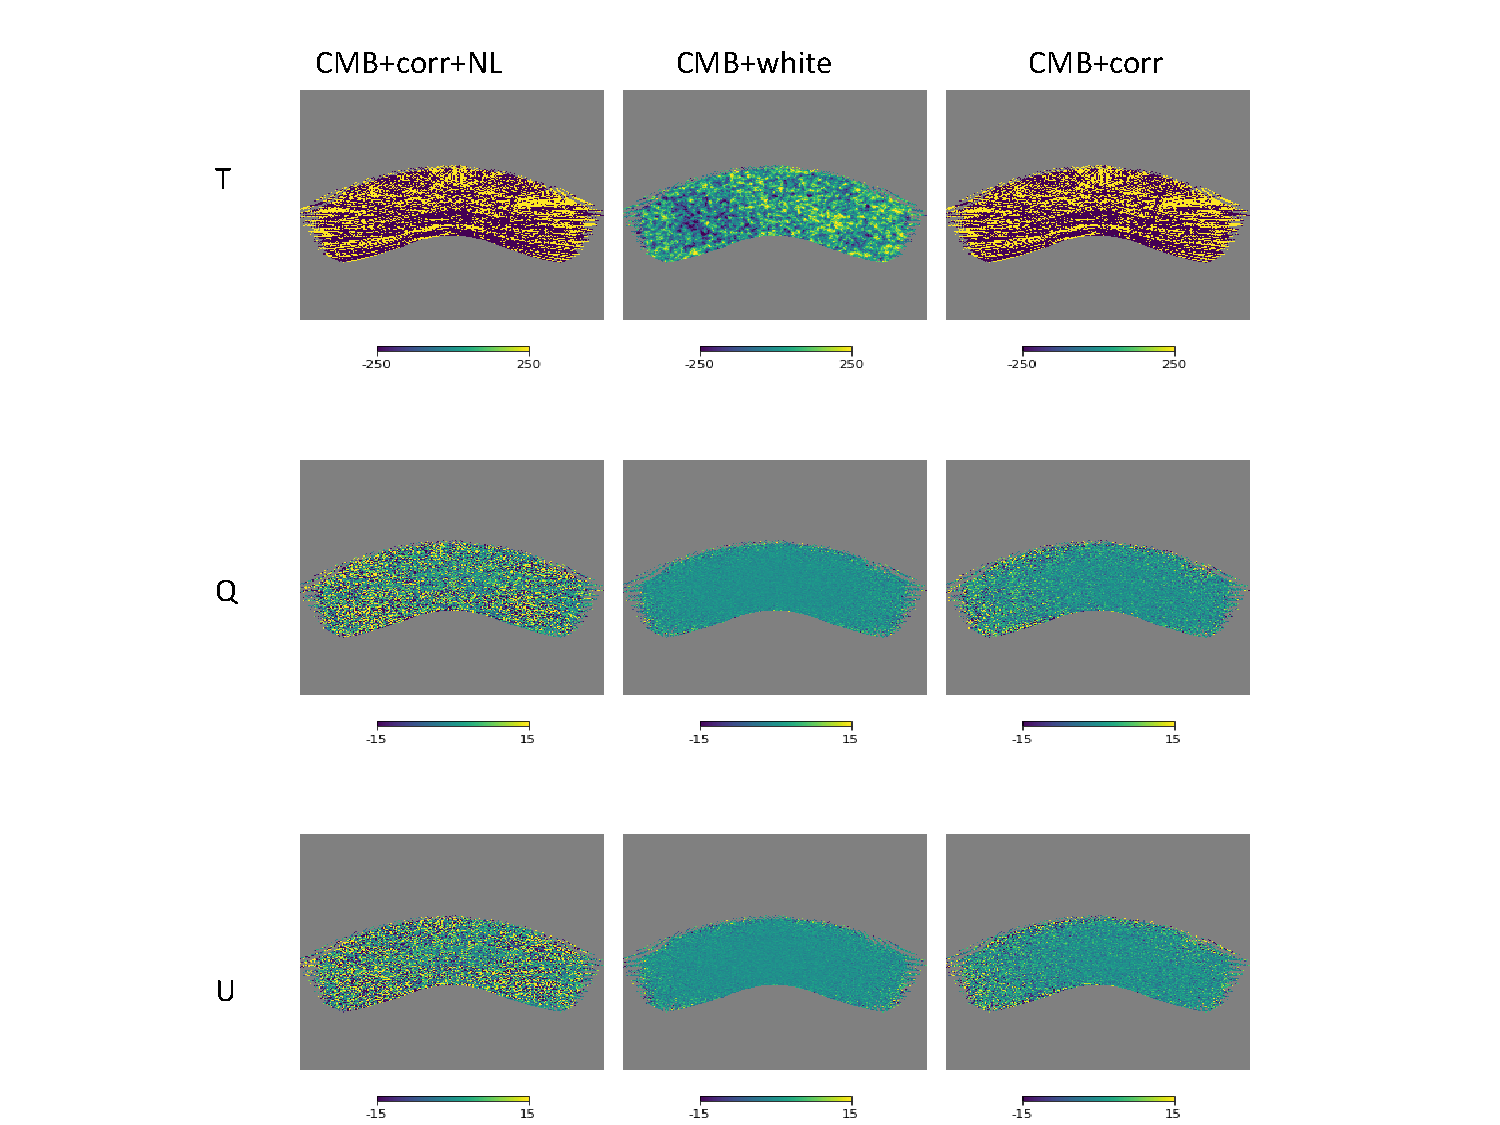
\includegraphics[width=0.85\textwidth]{figures/040218_s4cmb_corr_NL.pdf}
\caption{Pure T->P leakage maps generated with s4cmb for an example instrument and experiment. The middle column is pure CMB+white noise (minimal leakage), the right column is CMB+white+correlated noise, and the left is the same as the right but observed through the nonlinearity equation. Random draws of $g_1$ and $\tau_1$ were performed for each detector in the focal plane.}
\end{figure}

\paragraph{Uncertainty/Range:}
Current results from \cite{PB1_WHWP} quote rough estimates of $g_1 \sim$ 0.8 \%/K and $\tau_1 \sim$ 0.1 ms/K, where we assume $d(t)$ have been calibrated to CMB temperature using a conversion factor. Data for Advanced ACTPol detectors in the field with no sky loading show XX\% ratio of second-harmonic to first-harmonic amplitude.

\paragraph{Parameterization:}
We currently plan to use the simpler equation to determine what acceptable limits on $g_1$ and $\tau_1$ are demanded by science goals. When summarized in terms of TES design parameters, we can then feed these requirements back to the detector design group.
\subsection{Direct Pickup (Kevin)}

\paragraph{Description:}
Description of systematic effect, including relevant equations and
parameterization for TWGs. Note that each variable in each equation should be
defined. This should include where we expect to get the value of this variable
from (TWG, literature, etc.)

\paragraph{Plan to model and/or measure:}
Plan to model/measure effect. Use SRFs to describe how well we understand/can model the effect. Is there a good null test that we could use to catch this effect?

\paragraph{Uncertainty/Range:}
This section should include the uncertainty of
known parameters and/or the expected range of parameters for consideration

\paragraph{Parameterization:}
This section should include the parameterization of figures of
merit and the output to the SWGs.

\subsection{Array Non-Uniformity}

\paragraph{Description:}
In our estimates of array performance and sensitivity, we often assume that for an array with number of detectors $N_{\mbox{\scriptsize det}}$, each detector will have common signal-to-noise levels dominated by photon noise, and the sensitivity of the entire array scales as $\sim 1 / \sqrt{N_{\mbox{\scriptsize det}}}$. The measure of signal-to-noise for our detectors is noise-equivalent power, or $NEP$. For transition-edge sensor bolometers, this quantity is a function of parameters like the bias voltage used for each bolometer, the open loop gain $L$, and the thermal parameters $G$ and $T_{\mbox{\scriptsize c}}$, the thermal conductance and critical temperature, respectively, of each detector.

Beyond the TES bolometer itself, within-array variations of important optical parameters like thickness of dielectric layers, relevant to determining signal loss in microwave circuits and thus the optical efficiency of given pixels, have been observed. If we express this number as a temperature-to-power gain $\eta = dT/dP$, then variations in this number will lead to variations in the per-detector $NET$, or noise-equivalent temperature, of the detector. Since $NET \sim \eta NEP$, fluctuations in $\eta$ across the array are relevant for determining how sensitive the overall array is.

In general, achieving uniform sensitivity through fabrication engineering (especially relevant to $G$, $T_{\mbox{\scriptsize c}}$, and $\eta$) has a practical limit. For the former parameters, Advanced ACTPol arrays have shown a very tight distribution, which encourages us to focus on achieving uniform bias parameters over many parameters. \textbf{Add some info/plots on fab uniformity from Shannon's post (link in SPIE progress spreadsheet).} We only have control over the bias currents within ``bias lines'', which provide an identical current to hundreds of TES channels. Figure \ref{expect_biasability} shows the effect of moving from the 12 bias lines per frequency in Advanced ACTPol dichroic arrays to the 4 per frequency being designed in SO.

\begin{figure}[h!]
\centering
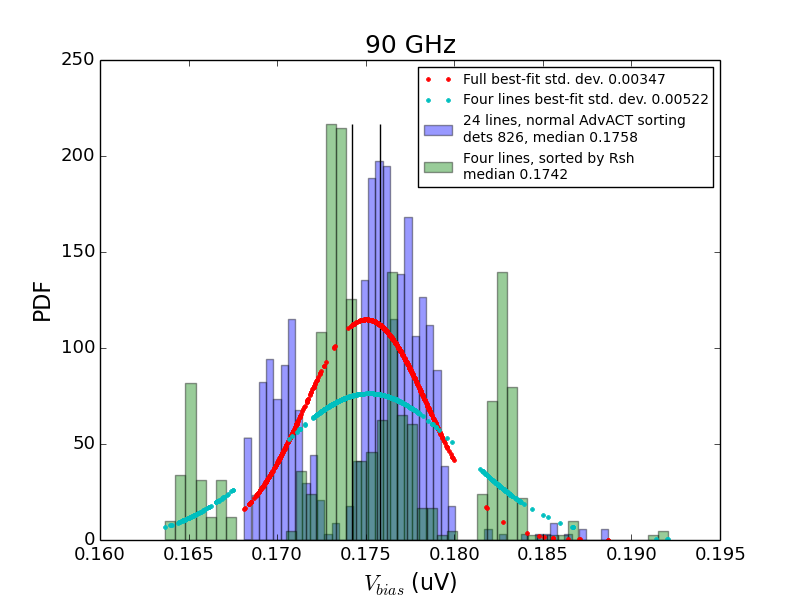
\includegraphics[width=0.4\textwidth]{figures/bias_volt_90GHz_ACTvsSO.png}\quad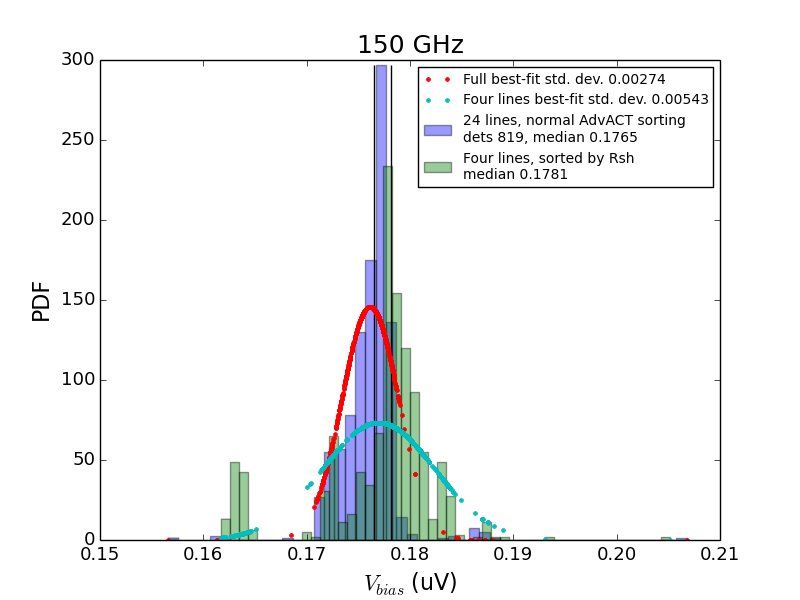
\includegraphics[width=0.4\textwidth]{figures/bias_volt_150GHz_ACTvsSO.png}
\caption{A bias uniformity proxy, detector bias voltage, for 90 and 150 GHz detectors in and AdvACT MF array. The two cases are with 12 bias lines and 4 bias lines per frequency, the latter being the planned for SO.}
\label{expect_biasability}
\end{figure}

However, all of these effects generally do not lead to systematic errors if calibrations are properly performed to bring each channel into agreement on the size of sky signals in CMB temperature units. We may worry more specifically about issues like nonuniform bandpass, but any science will come from array-wide averages of such effects. However, these variations can provide real limits on array performance if they fail to meet certain requirements. They can also set requirements on how well we need to calibrate certain dtector quantities as in the case of nonuniform bandpasses.

\paragraph{Plan to model and/or measure:}
SRF = 2. We have data specifiying the achieved distribution of thermal parameters measured widely across the array, as well as more limited results on efficiency, or $\eta$, and bandpasses. Tuning bias parameters uses as a proxy how well we achieve the target fraction of a detector's normal resistance $R_{\mbox{\scriptsize n}}$. Studying these statistics across a season is another way to learn how uniformly we are able to bias these detectors. Overall, these ``array health monitors'' do not cause systematics on their own, but require calibration issues to leak signal in. If all parameters are known for all channels, non-uniformity is not itself an issue. \textbf{How practical is it to say we should know it for all channels? Some come from IV curves, but others need specific calibration (like the bandpass), in which case measuring the full array may not be possible/practical. Make some comment here on practicality for different cases.} 

\paragraph{Uncertainty/Range:}
Current distributions of thermal parameters are tight, at a level of $\sim$ few \% [Ho SPIE 2016, Choi LTD 2017] \textbf{add these to the .bib file}. Strong trends with radius do not appear intrinsically. Projecting all of these numbers to array sensitivies [Choi LTD 2017] and comparing to the naive estimate based on $N_{\mbox{\scriptsize det}}$ averaging effects may be useful to determine the sensitivity hit.

\paragraph{Parameterization:}
We intend to calculate the sensitivity hit due to realistic nonuniformity around target parameters determined by the Detector TWG.




\section{Papers on systematics}

\input{tex/papers.tex}


 

%----------------------------------------------------------------------------------------
%	BIBLIOGRAPHY
%----------------------------------------------------------------------------------------

\renewcommand{\refname}{\spacedlowsmallcaps{References}} % For modifying the bibliography heading
\bibliographystyle{unsrt}
\bibliography{syst.bib} % The file containing the bibliography

%----------------------------------------------------------------------------------------

\end{document}
